% !TeX program = pdflatex
% Srpsko izdanje (probno: glave 0 do 5). Deli etf.cls, figures/, data/ i literaturu sa ../latex/.
% Build iz latex-sr/: TEXINPUTS=.:../latex: pdflatex x2 (vidi README.md u ovom folderu).
\documentclass[master,a4paper,12pt,oneside]{etf}

\usepackage[T1]{fontenc}
\usepackage[utf8]{inputenc}
\usepackage{lmodern}
\usepackage[a4paper, top=30mm, bottom=30mm, left=20mm, right=20mm]{geometry} % PPK margins
% Serbian last, so it is the document language and the text is hyphenated by Serbian patterns.
\usepackage[english,serbian]{babel}

\usepackage{graphicx}
\graphicspath{{../latex/figures/}{../latex/}}
\usepackage{amsmath}
\usepackage{amssymb}
\usepackage{booktabs}
\usepackage{tabularx}
\usepackage{xcolor}
\usepackage{listings}
\usepackage{tikz}
\usetikzlibrary{arrows.meta, positioning, fit, backgrounds}
\usepackage{pgfplots}
\pgfplotsset{compat=1.18}
\usepackage{microtype}
\usepackage[hidelinks]{hyperref}
\usepackage[nohyphen]{underscore} % literal _ in text/\texttt; break at _ without a hyphen
\setlength{\emergencystretch}{3em} % avoid right-margin overhang on hard-to-break code lines
\usepackage{needspace} % keep short atomic blocks (code listings) from splitting across pages

% Float packing. The defaults assume a text-heavy document and reserve at least 20% of every page for
% prose (\textfraction), which in a chapter with roughly one float per page pushes floats onto pages of
% their own and leaves large gaps. These let a page carry more float and less filler; the content is
% unchanged, only how densely it sets.
\renewcommand{\topfraction}{0.92}
\renewcommand{\bottomfraction}{0.75}
\renewcommand{\textfraction}{0.08}
\renewcommand{\floatpagefraction}{0.72}
\setcounter{topnumber}{3}
\setcounter{bottomnumber}{2}
\setcounter{totalnumber}{4}

% Widow/orphan control: don't strand a single line at the top/bottom of a page.
% Safe here because the class is \raggedbottom (oneside): slack goes to the page bottom.
\clubpenalty=10000
\widowpenalty=10000
\displaywidowpenalty=10000
\usepackage{fancyhdr}

% Nazivi strukture na srpskom (babel serbian daje ove nazive, ali eksplicitno radi doslednosti sa ../latex/).
\addto\captionsserbian{%
  \renewcommand{\contentsname}{Sadr\v{z}aj}%
  \renewcommand{\listfigurename}{Spisak slika}%
  \renewcommand{\listtablename}{Spisak tabela}%
  \renewcommand{\bibname}{Literatura}%
  \renewcommand{\figurename}{Slika}%
  \renewcommand{\tablename}{Tabela}%
  \renewcommand{\abstractname}{Sa\v{z}etak}%
  \renewcommand{\chaptername}{Glava}%
}

% PPK: page number in the bottom-right corner, on every page including chapter-opening (plain) pages.
\setlength{\headheight}{15pt}
\pagestyle{fancy}
\fancyhf{}
\renewcommand{\headrulewidth}{0pt}
\fancyfoot[R]{\thepage}
\fancypagestyle{plain}{\fancyhf{}\renewcommand{\headrulewidth}{0pt}\fancyfoot[R]{\thepage}}

% PPK: chapter titles UPPERCASE at ~20pt (\LARGE); the "Glava N" label at \large. ToC/bookmarks keep
% mixed case (they are written before \@makechapterhead runs).
\makeatletter
\renewcommand\@makechapterhead[1]{%
  \vspace*{50\p@}%
  {\parindent\z@ \raggedright \normalfont
    \ifnum \c@secnumdepth >\m@ne
      \large\bfseries \@chapapp\space\thechapter \par\nobreak \vskip 18\p@
    \fi
    \interlinepenalty\@M
    \LARGE\bfseries \MakeUppercase{#1}\par\nobreak \vskip 40\p@}}
\renewcommand\@makeschapterhead[1]{%
  \vspace*{50\p@}%
  {\parindent\z@ \raggedright \normalfont
    \interlinepenalty\@M
    \LARGE\bfseries \MakeUppercase{#1}\par\nobreak \vskip 40\p@}}
\makeatother

% Inline/code listing defaults (characteristic snippets, per PPK; not full code).
\lstset{basicstyle=\ttfamily\small, breaklines=true, columns=fullflexible,
        frame=single, captionpos=b, tabsize=2, showstringspaces=false}

% Reference title quotes. PPK specifies the Serbian „...“ pair; the thesis text is English, so the
% titles take English quotes and the one macro switches the whole bibliography either way.
\newcommand{\rqt}[1]{\textquotedblleft #1\textquotedblright}

% Both titles are registered on the topic-application form (master-rad/prijava/); the Serbian one leads
% here because this edition is in Serbian. Keep both in step with the form and with ../latex/main.tex.
\title{Hibridno osvetljenje u realnom vremenu primenom pra\'cenja zraka\\[0.6ex]
       {\large Real-Time Hybrid Lighting Using Ray Tracing}}
\author{Vuk \DJ or\dj evi\'c}
\indeks{2024/3102}
\mentor{prof. dr Dra\v{z}en Dra\v{s}kovi\'c}
% Revised edition: the cover says so (etf.cls prints \@date under "Beograd,"). The defended text is
% frozen unchanged in ../defended/.
\date{2026\\[1.5ex]{\normalsize revidirano izdanje, uz doprinos AI agenata}}

% Performance figures quoted in the text. Generated from the engine's committed perf baselines by
% tools/gen_perf_tables.py, never typed by hand: the previous hand-maintained data file drifted out
% of sync with a re-baseline and nothing detected it.
\newcommand{\perfFourEffectsAMD}{6.62}
\newcommand{\perfFourEffectsNV}{4.84}
\newcommand{\perfTotalAMD}{8.99}
\newcommand{\perfTotalNV}{6.15}
\newcommand{\perfBaseAMD}{2.37}
\newcommand{\perfBaseNV}{1.32}
\newcommand{\perfWidth}{1920}
\newcommand{\perfHeight}{1080}
\newcommand{\perfFrames}{300}
\newcommand{\perfEffShadowsAMD}{2.292}
\newcommand{\perfEffShadowsNV}{1.526}
\newcommand{\perfEffAoAMD}{0.859}
\newcommand{\perfEffAoNV}{0.775}
\newcommand{\perfEffReflAMD}{1.749}
\newcommand{\perfEffReflNV}{1.121}
\newcommand{\perfEffGiAMD}{1.717}
\newcommand{\perfEffGiNV}{1.413}
\newcommand{\perfNVSpread}{0.405}
\newcommand{\perfSsaoAMD}{0.505}
\newcommand{\perfSsaoNV}{0.336}
\newcommand{\perfSsrAMD}{0.513}
\newcommand{\perfSsrNV}{0.462}
\newcommand{\perfSsgiAMD}{0.763}
\newcommand{\perfSsgiNV}{0.920}
\newcommand{\perfTopEffectAMD}{shadows}
\newcommand{\perfTopResolvedAMD}{yes}
\newcommand{\perfUnresolvedPairsAMD}{1}
\newcommand{\perfUnresolvedAMD}{reflections and global illumination}
\newcommand{\perfUnresolvedGapAMD}{0.032}
\newcommand{\perfTopEffectNV}{shadows}
\newcommand{\perfTopResolvedNV}{no}
\newcommand{\perfUnresolvedPairsNV}{1}
\newcommand{\perfUnresolvedNV}{shadows and global illumination}
\newcommand{\perfUnresolvedGapNV}{0.113}
\newcommand{\perfGapBase}{1.06}
\newcommand{\perfGapGi}{2.84}
\newcommand{\perfRatioMin}{0.03}
\newcommand{\perfRatioMax}{2.20}
\newcommand{\perfShadowInlineAMD}{2.292}
\newcommand{\perfShadowStochAMD}{1.737}
\newcommand{\perfShadowGapAMD}{0.555}
\newcommand{\perfShadowRatioAMD}{1.3}
\newcommand{\perfShadowWinnerAMD}{stochastic}
\newcommand{\perfShadowInlineNV}{1.526}
\newcommand{\perfShadowStochNV}{3.340}
\newcommand{\perfShadowGapNV}{1.814}
\newcommand{\perfShadowRatioNV}{2.2}
\newcommand{\perfShadowWinnerNV}{inline}
\newcommand{\perfDenoiseAMD}{0.333}
\newcommand{\perfDenoiseNV}{0.313}

\newcommand{\rcGpuLow}{3.51}
\newcommand{\rcGpuHigh}{6.43}
\newcommand{\rcGpuPct}{83}
\newcommand{\rcPsnrGain}{0.20}
\newcommand{\rcFlipLow}{0.1486}
\newcommand{\rcFlipHigh}{0.1433}
\newcommand{\flickerOff}{0.2185}
\newcommand{\flickerOn}{0.2038}
\newcommand{\flickerPct}{6.7}
\newcommand{\hfSppOne}{10.8}
\newcommand{\hfSppTwo}{9.1}
\newcommand{\hfSppFour}{8.1}
\newcommand{\hfSppEight}{7.3}
\newcommand{\hfGiRaw}{41.7}
\newcommand{\hfGiDenoised}{1.5}
\newcommand{\hfConeSharp}{16.4}
\newcommand{\hfConeGlossy}{8.8}
\newcommand{\qRasterFlip}{0.435}
\newcommand{\qRasterPsnr}{15.14}
\newcommand{\qRasterSsim}{0.382}
\newcommand{\qRtGiFlip}{0.139}
\newcommand{\qRtGiPsnr}{25.36}
\newcommand{\qRtGiSsim}{0.721}
\newcommand{\qAllRtFlip}{0.086}
\newcommand{\qAllRtPsnr}{30.83}
\newcommand{\qAllRtSsim}{0.871}
\newcommand{\qRtLiftPsnr}{15.69}
\newcommand{\qSsgiFlip}{0.337}
\newcommand{\qRasterFlipLo}{0.363}
\newcommand{\qRasterFlipHi}{0.534}
\newcommand{\qRtGiFlipLo}{0.130}
\newcommand{\qRtGiFlipHi}{0.145}
\newcommand{\mAllRtTflip}{0.0082}
\newcommand{\mAllRtJod}{4.81}
\newcommand{\mAllRtLag}{0.104}
\newcommand{\mRtGiTflip}{0.0081}
\newcommand{\mRtGiJod}{3.89}
\newcommand{\mRtGiLag}{0.119}
\newcommand{\mRasterTflip}{0.0205}
\newcommand{\mRasterJod}{3.05}
\newcommand{\mRasterLag}{0.124}
\newcommand{\hrDeltaMs}{4.67}
\newcommand{\hrDeltaPct}{54}
\newcommand{\hrHalfTotal}{8.67}
\newcommand{\hrPsnrGain}{0.00}

\newcommand{\ommTotal}{64}
\newcommand{\ommOpaque}{26}
\newcommand{\ommTransparent}{24}
\newcommand{\ommUnknown}{14}
\newcommand{\ommHwPct}{78}

\newcommand{\rgaShaderCount}{47}
\newcommand{\rgaScratchBytes}{272}


\begin{document}

\maketitle

% --- Sa\v{z}etak + klju\v{c}ne re\v{c}i (PPK) ---
\begin{abstract}
Ovaj rad integri\v{s}e \v{c}etiri efekta osvetljenja zasnovana na pra\'cenju zrakova (senke,
ambijentalnu okluziju, refleksije i difuzno globalno osvetljenje) kao inline ray query
(\texttt{VK_KHR_ray_query}) prolaze preko rasterizacionog forward prolaza, u engine-u koji je autor
sam napisao kori\v{s}\'cenjem Vulkan API-ja. Rasterizacija te globalne efekte ina\v{c}e pribli\v{z}no
aproksimira postupcima u
prostoru ekrana i unapred izra\v{c}unatim postupcima, koji otkazuju na geometriji van ekrana i na
dinami\v{c}koj sceni. \v{S}umoviti signali se rekonstrui\v{s}u jednim zajedni\v{c}kim SVGF filtrom i
stabilizuju temporalnim anti-aliasing-om, dok senke na podrazumevanoj putanji ne zahtevaju prolaz za
uklanjanje \v{s}uma nego se vidljivost razre\v{s}ava inline tokom sen\v{c}enja. Cena svakog efekta na grafi\v{c}kom procesoru izoluje se
A/B matricom konfiguracija, a kvalitet rekonstrukcije meri se merama FLIP, PSNR i SSIM u odnosu na
konvergiranu path-traced referencu, preko vi\v{s}e ta\v{c}aka gledi\v{s}ta, na hardveru dva
proizvo\dj a\v{c}a (AMD RDNA4 i NVIDIA Blackwell) uz isti kod. Sva \v{c}etiri efekta zajedno ko\v{s}taju
\perfTotalAMD{} ms i \perfTotalNV{} ms po kadru na dve kartice, unutar bud\v{z}eta za 60 Hz, i
podi\v{z}u kvalitet rekonstrukcije sa FLIP \qRasterFlip{} na \qAllRtFlip{} i PSNR \qRasterPsnr{} na
\qAllRtPsnr{} dB u odnosu na referencu. Dva proizvo\dj a\v{c}a se ne sla\v{z}u oko toga koji je efekat
najskuplji, na RX 9070 XT su to senke a na RTX 5070 globalno osvetljenje, i to neslaganje se prenosi
na in\v{z}enjersku odluku: od dve implementirane strategije za senke, stohasti\v{c}ka je jeftinija na
AMD-u a \perfShadowRatioNV{} puta skuplja na NVIDIA-i, pa je renderer koji fiksira bilo koju od njih
pogre\v{s}an na jednoj od ove dve kartice aktuelne generacije. Merenje na jednom proizvo\dj a\v{c}u to
ne bi otkrilo.
\end{abstract}

\begin{keywords}
ray tracing u realnom vremenu; ray query; Vulkan; globalno osvetljenje; ambijentalna okluzija;
refleksije; SVGF; uklanjanje \v{s}uma; hibridno renderovanje; cross-vendor; AMD RDNA4; NVIDIA Blackwell
\end{keywords}

% PPK: front matter in roman numerals; arabic count restarts at Uvod.
\pagenumbering{roman}

\tableofcontents

\clearpage \phantomsection \addcontentsline{toc}{chapter}{\listfigurename}
\listoffigures

\clearpage \phantomsection \addcontentsline{toc}{chapter}{\listtablename}
\listoftables

\chapter*{Spisak skra\'cenica}
\addcontentsline{toc}{chapter}{Spisak skra\'cenica}

\begin{description}
  \item[AO] Ambient Occlusion (ambijentalna okluzija): zatamnjenje tamo gde obli\v{z}nja geometrija
    blokira difuznu svetlost, npr. u uglovima i pukotinama
  \item[\`a-trous] filter koji u svakoj iteraciji udvostru\v{c}uje razmak izme\dj u uzoraka, pa
    dopire \v{s}ire bez kvadratnog rasta cene
  \item[bindless] svaka tekstura i bafer u sceni izlo\v{z}eni kao jedan veliki indeksirani niz, pa
    \v{s}ejder mo\v{z}e da adresira resurs celobrojnim indeksom umesto da on bude vezan za
    konkretan poziv crtanja
  \item[BLAS] Bottom-Level Acceleration Structure: BVH nad trouglovima jedne mre\v{z}e, u prostoru
    objekta
  \item[blue noise] niz \v{c}ija je gre\v{s}ka koncentrisana na visokim frekvencijama, pa susedni
    pikseli i uzastopni kadrovi dobijaju namerno raznorodne uzorke, zbog \v{c}ega prosek preko njih
    br\v{z}e konvergira
  \item[BRDF] Bidirectional Reflectance Distribution Function: opisuje koliko svetlosti povr\v{s}
    odbija iz jednog smera u drugi
  \item[BVH] Bounding Volume Hierarchy: stablo ugnje\v{z}denih kutija koje omogu\'cava zraku da
    presko\v{c}i ve\'cinu trouglova
  \item[CVar] Console Variable
  \item[DDGI] Dynamic Diffuse Global Illumination
  \item[disokluzija] piksel koji u prethodnom kadru nije bio vidljiv, pa ne postoji istorija koju
    temporalni filter mo\v{z}e da iskoristi
  \item[ECS] Entity-Component-System
  \item[FLIP] perceptivna mera razlike izme\dj u slika (NVIDIA), ni\v{z}a vrednost je bolja
  \item[G-bafer] me\dj ubafer sa geometrijskim podacima po pikselu (dubina, normala), popunjen pre
    sen\v{c}enja
  \item[GI] Global Illumination (globalno osvetljenje): svetlost koja stigne do povr\v{s}i posle
    najmanje jednog odbijanja
  \item[HLSL] High-Level Shading Language
  \item[JOD] Just-Objectionable-Difference: jedinica mere ColorVideoVDP, gde razlika od oko 1 JOD
    odgovara otprilike 75\% preferencije populacije izme\dj u dve slike
  \item[ka\v{s}njenje (lag)] koliko slika u pokretu zaostaje za sopstvenom konvergiranom mirnom slikom
    sa istom pozicijom kamere, mera temporalnog razmazivanja a ne ta\v{c}nosti
  \item[LDS] Local Data Share: deljena memorija radne grupe na AMD grafi\v{c}kim procesorima
  \item[MIS] Multiple Importance Sampling
  \item[NEE] Next-Event Estimation: kod path tracer-a, uzorkovanje izvora svetlosti direktno iz
    svakog temena putanje umesto \v{c}ekanja da ga zrak slu\v{c}ajno pogodi
  \item[OMM] Opacity Micromap: mapa neprozirnosti po mikro-trouglu koja omogu\'cava obilasku da
    presko\v{c}i alfa test
  \item[penumbra] meki prelaz izme\dj u osvetljenog dela i pune senke (umbre), \v{s}iri \v{s}to je
    izvor svetlosti ve\'ci ili zaklanja\v{c} dalji
  \item[PSNR] Peak Signal-to-Noise Ratio: logaritamska mera srednje kvadratne gre\v{s}ke, ve\'ca
    vrednost je bolja, mada sistemati\v{c}no favorizuje zamu\'cenu sliku
  \item[radijansa] svetlosna energija po jedinici projektovane povr\v{s}ine i jedinici prostornog
    ugla, veli\v{c}ina koju piksel na kraju \v{c}uva. Iradijansa je ista energija integrisana po
    dolaznim smerovima, bez sopstvenog smera
  \item[RDNA] Radeon DNA (arhitektura AMD grafi\v{c}kih procesora)
  \item[reprojekcija] preslikavanje piksela iz teku\'ceg kadra u prethodni preko vektora kretanja,
    radi ponovne upotrebe ranije izra\v{c}unatog rezultata
  \item[ReSTIR] Reservoir Spatiotemporal Importance Resampling
  \item[RIS] Resampled Importance Sampling
  \item[RT] Ray Tracing
  \item[RTXGI] RTX Global Illumination
  \item[SIMD / SM] jedinica raspore\dj iva\v{c}a koja dr\v{z}i vi\v{s}e talasa (AMD) ili warp-ova
    (NVIDIA) rezidentnih istovremeno i izdaje instrukcije iz njih
  \item[SPIR-V] Standard Portable Intermediate Representation (Vulkan)
  \item[spp] uzoraka po pikselu
  \item[SSAO] Screen-Space Ambient Occlusion
  \item[SSGI] Screen-Space Global Illumination
  \item[SSIM] Structural Similarity Index Measure: poredi lokalnu strukturu a ne apsolutne
    vrednosti, ve\'ca vrednost je bolja
  \item[SSR] Screen-Space Reflections
  \item[SVGF] Spatiotemporal Variance-Guided Filtering: uklanja\v{c} \v{s}uma koji kombinuje
    temporalnu akumulaciju sa prostornim filterom vo\dj enim procenjenom varijansom
  \item[TAA] Temporal Anti-Aliasing
  \item[tFLIP] temporalni FLIP: koliko se tehnika menja izme\dj u susednih kadrova preko onoga koliko
    se referenca menja u istom intervalu, pa stabilan rezultat dobija nisku vrednost
  \item[TLAS] Top-Level Acceleration Structure: BVH nad instancama, gde svaka instanca nosi
    transformaciju i pokaziva\v{c} na BLAS
  \item[tonemap] preslikavanje HDR vrednosti u opseg ekrana
  \item[VGPR] Vector General-Purpose Register: registri po niti \v{c}ija brojnost odre\dj uje koliko
    talasa mo\v{z}e istovremeno da bude u letu (zauzetost)
  \item[visokofrekventna energija] udeo signala bafera u finom detalju a ne u \v{s}irokim
    gradijentima, ovde kori\v{s}\'cen da se izmeri koliko je filter zamutio sliku
  \item[Vulkan] niskonivojski grafi\v{c}ki i compute API, nezavisan od proizvo\dj a\v{c}a, na kome je
    ovaj engine izgra\dj en i u kome je pra\'cenje zraka opciono pro\v{s}irenje a ne deo jezgra
  \item[wave / warp] grupa niti koje izvr\v{s}avaju istu instrukciju u koraku, na AMD-u se zove wave a
    na NVIDIA-i warp. Warp uvek ima 32 niti; RDNA bira 32 ili 64 po \v{s}ejderu, a drajver za compute
    \v{s}ejdere ovog engine-a prijavljuje 64
  \item[zauzetost (occupancy)] broj istovremeno aktivnih talasa po SIMD jedinici: ve\'ca zauzetost
    bolje skriva latenciju memorije
  \end{description}


\clearpage % ship the last roman (front-matter) page before switching to arabic
\pagenumbering{arabic}
\chapter{Uvod}
\label{ch:uvod}

\section{Problem i motivacija}

Renderovanje u realnom vremenu dominantno se zasniva na rasterizaciji, koja veoma efikasno
razre\v{s}ava primarnu vidljivost (\v{s}ta kamera neposredno vidi), ali nema nikakav prirodan pojam o tome
\v{s}ta bilo koja ta\v{c}ka povr\v{s}i vidi izvan sebe. Efekti po kojima slika deluje verodostojno zavise upravo
od toga: indirektno osvetljenje koje se odbija izme\dj u povr\v{s}i, kontaktne senke, sjajne refleksije i
ambijentalna okluzija svi odgovaraju na pitanje \quotedblbase{}\v{s}ta je jo\v{s} vidljivo odavde\textquotedblright{}. Engine-i za
renderovanje u realnom vremenu odavno ih aproksimiraju. Metode u prostoru ekrana (SSAO, refleksije i
globalno osvetljenje u prostoru ekrana) su jeftine, ali vide samo ono \v{s}to je trenutno na ekranu, pa
otkazuju kad je potrebna geometrija van ekrana ili tek otkrivena disokluzijom
\cite{mittring2007cryengine, bavoil2008hbao}. Prora\v{c}unate metode pe\v{c}u osvetljenje u lightmape ili
probe i ne mogu da prate dinami\v{c}ku geometriju. Voksel pristupi, kao \v{s}to je voxel cone tracing, pokrivaju
celu scenu, ali su grubi i skloni curenju svetlosti \cite{crassin2011vxgi}.

Hardversko pra\'cenje zrakova menja ono \v{s}to je isplativo. GPU-ovi od NVIDIA RTX (2018) i AMD RDNA2 (2020)
imaju namenske jedinice za obilazak hijerarhije grani\v{c}nih zapremina (BVH) i presek zraka i trougla, pa je
zrak prema celoj sceni dovoljno jeftin da se baca po pikselu interaktivnom brzinom. Navedeni efekti
postaju fizi\v{c}ki zasnovani prolazi koji uzorkuju stvarnu scenu umesto proksija u prostoru ekrana.
Problem je cena. Direktno re\v{s}avanje jedna\v{c}ine renderovanja \cite{kajiya1986rendering} path tracing-om,
koji integrali svetlost koja sti\v{z}e u ta\v{c}ku povr\v{s}i iz svih pravaca, ostaje daleko izvan bud\v{z}eta
realnog vremena pri rezoluciji ekrana. Prihvatljiv bud\v{z}et je jedan ili nekoliko zrakova po pikselu, \v{s}to
uzorkuje samo mali deo putanja svetlosti koje sti\v{z}u u piksel, pa je procena ta\v{c}na u proseku, ali ne i po
pikselu. Ta gre\v{s}ka je \v{s}um. Prakti\v{c}an put, kojim ide i ovaj rad, zato je hibridan: primarna
vidljivost se rasterizuje, sekundarni efekti se dodaju kao prolazi sa pra\'cenjem zrakova pri malom broju
uzoraka, a \v{c}ista slika se rekonstrui\v{s}e uklanjanjem \v{s}uma \cite{schied2017svgf}
(Slika~\ref{fig:teaser}).

\begin{figure}[tbp]
\centering
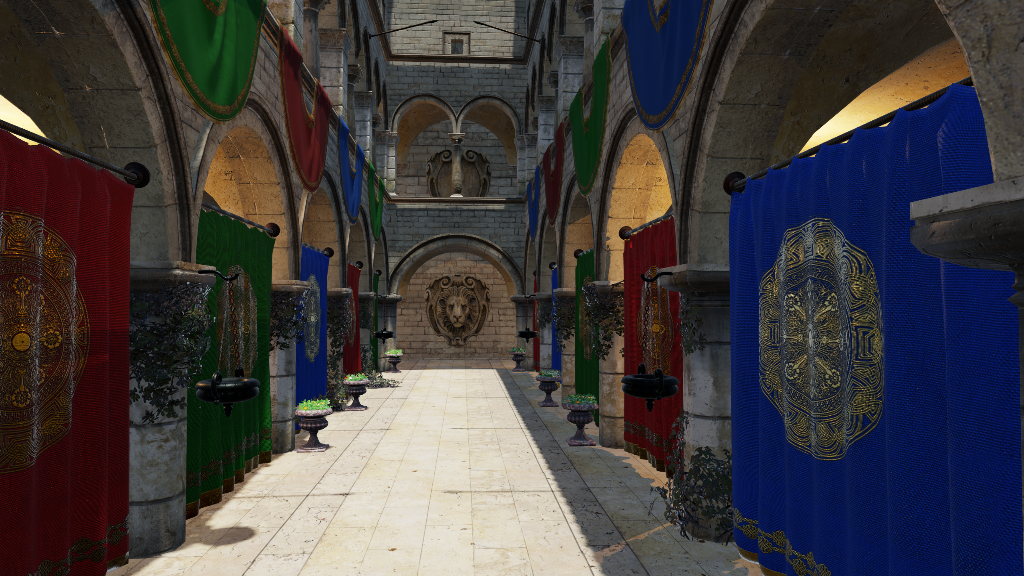
\includegraphics[width=0.92\textwidth]{figures/teaser_raster.png}\\[2mm]
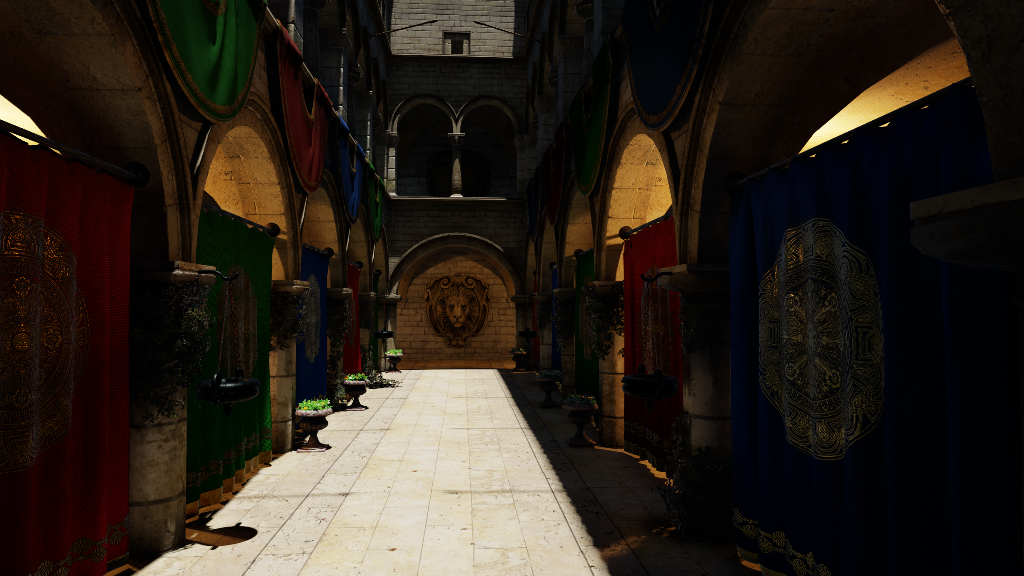
\includegraphics[width=0.92\textwidth]{figures/teaser.png}
\caption[Isti kadar rasterizovan i sa osvetljenjem zasnovanim na pra\'cenju zrakova]{Isti kadar, kamera i
ekspozicija na test sceni (Sponza). \textbf{Gore:} sam rasterizovani forward prolaz, u kome konstantan
ambijentalni \v{c}lan zamenjuje sve \v{s}to svetlost radi posle prvog odbijanja. \textbf{Dole:} isti prolaz sa
senkama, ambijentalnom okluzijom, refleksijama i globalnim osvetljenjem zasnovanim na pra\'cenju zrakova.
Gornja slika je svetlija, \v{s}to je i poenta: njen ambijentalni \v{c}lan podjednako podi\v{z}e svaku povr\v{s}inu,
osvetljenu ili ne, dok ga na donjoj zamenjuje svetlost koja je stvarno pre\v{s}la put.}
\label{fig:teaser}
\end{figure}

\section{Za\v{s}to hibridni pristup i za\v{s}to ray query (a ne RT pipeline)}

Vulkan nudi dva na\v{c}ina za pra\'cenje zrakova: namenski ray tracing pipeline i inline ray query
(\texttt{VK_KHR_ray_query}). Odeljak~\ref{sec:vulkanrt} ih poredi.

Ovaj rad koristi inline ray query iz razloga arhitektonske uklopljenosti: engine je rasterizacioni forward
renderer, a inline upiti omogu\'cavaju da se svaki efekat ubaci kao obi\v{c}an compute ili fragment prolaz,
bez preure\dj{}ivanja renderera oko ray tracing pipeline-a i njegove tabele vezivanja. Efekti se mogu
dodavati jedan po jedan, \v{s}to odgovara hibridnom dizajnu u kome su zraci ciljani dodatak rasterizaciji, a
ne primarna arhitektura. Cena je to \v{s}to se rad sa zracima ne mo\v{z}e preure\dj{}ivati izme\dj u invokacija
\v{s}ejdera radi o\v{c}uvanja koherentnosti divergentnih putanja, i to \v{s}to rekurzija mora biti eksplicitna
petlja, a ne \v{s}ejder koji pokre\'ce novi zrak. Efekti ovde su plitki (jedno odbijanje), pa je druga cena
mala.

\section{Cilj i istra\v{z}iva\v{c}ko pitanje}

Cilj je da se implementiraju \v{c}etiri efekta osvetljenja zasnovana na pra\'cenju zrakova: senke,
ambijentalna okluzija, refleksije i difuzno globalno osvetljenje, kroz inline ray query u sopstvenom Vulkan
engine-u, i da se svaki od njih okarakteri\v{s}e. Istra\v{z}iva\v{c}ko pitanje se razla\v{z}e na merljiva potpitanja:
cena svakog efekta na GPU-u u milisekundama; uticaj broja uzoraka po pikselu na kvalitet (PSNR/SSIM) i na
vreme; kvalitet i cena uklanjanja \v{s}uma kad je uklju\v{c}eno u odnosu na isklju\v{c}eno; uticaj pra\'cenja zrakova pri
polovini u odnosu na punu rezoluciju; i kako se identi\v{c}na Vulkan implementacija pona\v{s}a na GPU-ovima
razli\v{c}itih proizvo\dj{}a\v{c}a (AMD RDNA4 prema NVIDIA Blackwell). Obim je namerno ograni\v{c}en: jedna
zatvorena scena (Sponza), dva GPU-a aktuelne generacije sli\v{c}nog ranga (Tabela~\ref{tab:gpus}), difuzno
globalno osvetljenje i konvergirana path-traced referenca za metrike kvaliteta.

Tri odgovora protivre\v{c}e intuiciji. Osam puta ve\'ci bud\v{z}et zrakova donosi samo \rcPsnrGain{} dB PSNR-a.
Dobitak je stvaran, jer pribli\v{z}no tri puta prema\v{s}uje prag merenja, ali ko\v{s}ta \rcGpuPct\% vi\v{s}e GPU
vremena, pa radnu ta\v{c}ku postavlja na jedan zrak po pikselu (Odeljak~\ref{sec:raycount}). Uklanjanje
\v{s}uma se isplati u temporalnoj stabilnosti, a ne u stati\v{c}koj vernosti (Odeljak~\ref{sec:motion}). I
\v{s}ejder koji nosi inline upit za senke zauzima 130 registara prema 87 bez njega, \v{s}to prelazi granicu
alokacije i spu\v{s}ta ga sa 16 istovremeno rezidentnih talasa na 10, a upravo tu se cena tog upita
stati\v{c}ki vidi (Odeljak~\ref{sec:occupancy}).

\section{Doprinosi}

Doprinosi su:

\begin{itemize}
\item integrisana implementacija \v{c}etiri hibridna efekta osvetljenja zasnovana na ray query-ju, otvorene
licence, u jednom sopstvenom Vulkan engine-u;
\item raspodela cene GPU-a po efektima dobijena ponovljivim A/B benchmark okvirom, a ne ad hoc
snimcima;
\item ponovo upotrebljiv obrazac sa polovinom rezolucije, prepass-om G-bafera, uklanjanjem \v{s}uma i
upsampling-om;
\item evaluacija sopstvene implementacije SVGF filtera koji dele svi signali kojima je potreban: kvalitet
koji vra\'ca, cena i temporalna stabilnost;
\item pore\dj{}enje performansi istog koda identi\v{c}nog ray query pipeline-a na AMD RDNA4 i NVIDIA Blackwell
hardveru, koje pokazuje da se rang dve strategije senki me\dj{}u proizvo\dj{}a\v{c}ima obr\'ce
(Odeljak~\ref{sec:analiza-shadow-strategy}, Tabela~\ref{tab:shadow-strategy}): stohasti\v{c}ka strategija
pobe\dj{}uje za \perfShadowGapAMD{} ms na RX 9070 XT, a gubi za faktor \perfShadowRatioNV{} na RTX 5070.
\end{itemize}

\section{Struktura rada}

Glava~\ref{ch:pregled} daje pregled teorijskih osnova (rasterizacija prema pra\'cenju zrakova, strukture
ubrzanja, Vulkan ekstenzije za pra\'cenje zrakova) i postoje\'ca re\v{s}enja u realnom vremenu sa kojima se
evaluacija poredi. Glava~\ref{ch:implementacija} opisuje implementaciju: engine i graf renderovanja,
izgradnju struktura ubrzanja, \v{c}etiri efekta, SVGF filter, temporalni resolve i alate za merenje.
Glava~\ref{ch:analiza} izoluje cenu svakog efekta i meri kvalitet rekonstrukcije u odnosu na referencu i na
postoje\'ca re\v{s}enja iz Glave~\ref{ch:pregled}. Glava~\ref{ch:zakljucak} iznosi ograni\v{c}enja i
pravce daljeg rada.

\chapter{Pregled postoje\'cih re\v{s}enja i tehnologija}
\label{ch:pregled}


\section{Rasterizacija naspram pra\'cenja zraka}
\label{sec:rastervsrt}

Rasterizacija projektuje svaki trougao na ravan slike i vidljivost razre\v{s}ava baferom dubine. To je
operacija nad tokom podataka koja se dobro preslikava na GPU hardver, ali obra\dj uje jedan trougao po
jedan, bez pristupa ostatku scene, pa ne mo\v{z}e prirodno da odgovori na pitanje \quotedblbase{}\v{s}ta je
jo\v{s} vidljivo iz ove ta\v{c}ke\textquotedblright{}. Pra\'cenje zraka (ray tracing) umesto toga ba\v{c}a zrake u scenu i
nalazi njihove najbli\v{z}e preseke \cite{moller1997raytri}, a transport svetlosti procenjuje uzorkovanjem
\cite{pharr2016pbrt}. Time se razre\v{s}ava vidljivost izme\dj u proizvoljnih ta\v{c}aka, \v{s}to zahtevaju
indirektno osvetljenje, refleksije i okluzija, po ceni obilaska strukture po zraku i \v{s}uma uzorkovanja.

Zajedni\v{c}ka referenca za oba pristupa je jedna\v{c}ina renderovanja \cite{kajiya1986rendering}. Ona deli
izlaznu radijansu $L_o$ u ta\v{c}ki $\mathbf{x}$ u pravcu $\omega_o$ na emitovanu radijansu i reflektovani
integral preko hemisfere $\Omega$, pri \v{c}emu je radijansa energija svetlosti po jedinici projektovane
povr\v{s}ine i jedinici prostornog ugla, fizi\v{c}ka veli\v{c}ina koju piksel na kraju skladi\v{s}ti:
\begin{equation}
L_o(\mathbf{x}, \omega_o) = L_e(\mathbf{x}, \omega_o) + \int_{\Omega}
f_r(\mathbf{x}, \omega_i, \omega_o)\, L_i(\mathbf{x}, \omega_i)\, (\omega_i \cdot \mathbf{n})\,
\mathrm{d}\omega_i,
\label{eq:rendering}
\end{equation}
gde je $f_r$ BRDF, $L_i$ dolazna radijansa, a $\mathbf{n}$ normala povr\v{s}i.
Rasterizacija efikasno razre\v{s}ava emitovani i direktni \v{c}lan projekcijom, ali integral zahteva
dolaznu radijansu iz svih pravaca, dakle vidljivost u celoj sceni, \v{s}to rasterizacija ne mo\v{z}e da
izrazi, a pra\'cenje zraka procenjuje uzorkovanjem. Hibridni renderer koristi svaki pristup tamo gde je
jak (Slika~\ref{fig:rastervsrt}) \cite{akenine2018rtr}.

\begin{figure}[tbp]
\centering
\begin{tikzpicture}[>={Stealth[]}, scale=0.9]
  \begin{scope}
    \node[font=\small] at (1.9,3.1) {Rasterizacija};
    \fill (0,1.3) circle (1.6pt) node[left, font=\scriptsize] {oko};
    \draw[thick] (1,0.35) -- (1,2.35); \node[font=\scriptsize] at (1,0.05) {ravan slike};
    \draw[fill=black!8] (3.4,0.7) -- (4.0,2.1) -- (2.8,1.95) -- cycle;
    \draw[black!55] (0,1.3) -- (3.4,0.7);
    \draw[black!55] (0,1.3) -- (4.0,2.1);
    \draw[black!55] (0,1.3) -- (2.8,1.95);
    \node[font=\scriptsize] at (3.5,2.4) {trougao};
  \end{scope}
  \begin{scope}[xshift=6.4cm]
    \node[font=\small] at (1.9,3.1) {Pra\'cenje zraka};
    \fill (0,1.3) circle (1.6pt) node[left, font=\scriptsize] {oko};
    \draw[thick] (1,0.35) -- (1,2.35); \node[font=\scriptsize] at (1,0.05) {ravan slike};
    \fill[black!8] (3.5,1.3) circle (0.5);
    \draw[->, black!70] (0,1.3) -- (2.95,1.3);
    \node[font=\scriptsize] at (2.0,1.55) {zrak};
  \end{scope}
\end{tikzpicture}
\caption[Rasterizacija naspram pra\'cenja zraka]{Rasterizacija (projekcija trouglova na ravan slike) naspram pra\'cenja zraka (zrak kroz
piksel u scenu do najbli\v{z}eg preseka).}
\label{fig:rastervsrt}
\end{figure}

\section{Strukture ubrzanja: BVH, TLAS/BLAS}
\label{sec:accel-pregled}

Testiranje svakog zraka protiv svakog trougla je $O(\text{zraka} \times \text{trouglova})$ i bezizlazno na
razmeri scene, pa pra\'cenje zraka zavisi od prostorne strukture ubrzanja. Standardna je hijerarhija
grani\v{c}nih zapremina (BVH): stablo ugnje\v{z}denih grani\v{c}nih kutija \v{c}iji obilazak silazi samo u kutije u
koje zrak zaista ulazi, \v{s}to o\v{c}ekivanu cenu po zraku svodi na pribli\v{z}no logaritamsku u broju
trouglova (Slika~\ref{fig:bvh}).

\begin{figure}[tbp]
\centering
\begin{tikzpicture}[>={Stealth[]}, font=\small,
  tri/.style={draw, fill=black!12},
  bx/.style={draw, rounded corners=1pt, thick},
  nd/.style={draw, rounded corners, minimum width=7mm, minimum height=5mm, font=\scriptsize,
             inner sep=2pt},
  hit/.style={nd, fill=black!12},
  skip/.style={nd, densely dashed, text=black!45, draw=black!45}]

  \begin{scope}
    \node[font=\small] at (2.5,4.0) {scena u kutijama};
    \draw[bx, black!45] (0.15,0.15) rectangle (4.85,3.5);
    \node[font=\scriptsize, black!45] at (4.62,3.28) {A};
    \draw[bx] (0.35,0.4) rectangle (2.3,3.05);  \node[font=\scriptsize] at (0.6,2.82) {B};
    \draw[bx] (2.6,0.4) rectangle (4.65,3.05);  \node[font=\scriptsize] at (2.85,2.82) {C};
    \draw[tri] (0.7,0.8) -- (1.5,0.8) -- (1.1,1.6) -- cycle;
    \draw[tri] (1.2,1.9) -- (2.05,1.9) -- (1.6,2.7) -- cycle;
    \draw[tri] (2.9,0.8) -- (3.7,0.8) -- (3.3,1.6) -- cycle;
    \draw[tri] (3.6,1.9) -- (4.4,1.9) -- (4.0,2.7) -- cycle;
    % zrak ulazi u A i B, potpuno promasuje C, pa se podstablo C nikad ne otvara
    \draw[->, very thick] (-0.5,1.15) -- (2.35,1.15);
    \node[font=\scriptsize] at (-0.1,1.45) {zrak};
  \end{scope}

  \begin{scope}[xshift=7.2cm, yshift=0.35cm]
    \node[font=\small] at (1.6,3.65) {stablo koje obilazi};
    \node[hit]  (a)  at (1.6,3.0) {A};
    \node[hit]  (b)  at (0.6,2.0) {B};
    \node[skip] (c)  at (2.6,2.0) {C};
    \node[hit]  (t1) at (0.1,1.0) {$\triangle$};
    \node[skip] (t2) at (1.1,1.0) {$\triangle$};
    \node[skip] (t3) at (2.1,1.0) {$\triangle$};
    \node[skip] (t4) at (3.1,1.0) {$\triangle$};
    \draw (a) -- (b); \draw[black!45] (a) -- (c);
    \draw (b) -- (t1); \draw[black!45] (b) -- (t2);
    \draw[black!45] (c) -- (t3); \draw[black!45] (c) -- (t4);
    \node[font=\scriptsize, align=left] at (1.6,0.25)
      {senka\v{c}eno = kutija u koju se ulazi, testirana\\isprekidano = nikad otvoreno};
  \end{scope}
\end{tikzpicture}
\caption[Kako hijerarhija grani\v{c}nih zapremina u\v{s}tedi rad]{Hijerarhija grani\v{c}nih zapremina nad \v{c}etiri trougla.
Svaka kutija obuhvata sve ispod sebe, pa zrak koji proma\v{s}i kutiju ne mo\v{z}e pogoditi ni\v{s}ta unutar nje i
celo podstablo se presko\v{c}i bez ijednog testa trougla. Ovde zrak ulazi u A i B, a proma\v{s}i C, pa testira jedan
trougao umesto \v{c}etiri. Prave hijerarhije su dublje i \v{s}ire, \v{s}to taj odnos pretvara u pribli\v{z}no
logaritamsku umesto linearne cene, a dve GPU se razlikuju po tome ko obilazi stablo, a ne po njegovom
obliku (Slika~\ref{fig:traversal}).}
\label{fig:bvh}
\end{figure} Koliko dobro dato stablo radi zavisi od toga gde su postavljene podele, koje se biraju
heuristikom cene (naj\v{c}e\v{s}\'ce heuristikom povr\v{s}ine, koja favorizuje podele nakon kojih je malo verovatno da zrak
ude u oba deteta). Na ovom hardveru stablo gradi drajver i on bira heuristiku, pa to nije parametar koji ovaj rad
postavlja. Na dana\v{s}njim GPU testovi zrak-kutija i zrak-trougao rade u fiksnoj hardverskoj funkciji, \v{s}to
\v{c}ini zrak po pikselu pristupa\v{c}nim u realnom vremenu. Koliki je deo \emph{obilaska} oko tih testova tako\dj e
fiksna funkcija, razlikuje se po proizvo\dj a\v{c}u, a dve GPU ocenjene u glavi~\ref{ch:analiza} nalaze se na
suprotnim stranama te granice (Slika~\ref{fig:traversal}): NVIDIA RT jezgra obilaze hijerarhiju u hardveru
\cite{nvidia_turing}, dok se na AMD RDNA arhitekturama petlja obilaska izvr\v{s}ava shader instrukcijama koje
izdaju hardverske testove preseka \cite{amd_rdna_isa}, pa obilazak sa sen\v{c}enjem deli iste izvr\v{s}ne resurse.
To je strukturni razlog da se \emph{o\v{c}ekuje} da isti shader ko\v{s}ta razli\v{c}ito na dva proizvo\dj a\v{c}a, a ne
pripisivanje uzroka. Odeljak~\ref{sec:cena} meri odnos cene po prolazu AMD/NVIDIA koji u konfiguraciji
\texttt{+gi} obuhvata raspon od \perfRatioMin{} do \perfRatioMax{}, pa razlika nije jedan globalni faktor
takta. Ova evaluacija ne izoluje koliki deo te razlike poti\v{c}e od ovog mehanizma, a koliki od takta,
ke\v{s}a ili drajvera.

\begin{figure}[tbp]
\centering
\begin{tikzpicture}[>={Stealth[]}, font=\small,
  unit/.style={draw, rounded corners, align=center, minimum width=2.6cm, minimum height=9mm},
  fixed/.style={unit, fill=black!8}]
  \begin{scope}
    \node[font=\small\bfseries] at (1.9,3.5) {NVIDIA (RT jezgra)};
    \node[unit] (sm) at (1.9,2.5) {SM / shader};
    \node[fixed, below=12mm of sm, minimum height=14mm, text width=2.4cm] (rtc)
      {RT jezgro:\\obilazak \emph{i} preseci};
    \draw[->] ([xshift=-9mm]sm.south) -- node[left, font=\scriptsize] {1 zrak} ([xshift=-9mm]rtc.north);
    \draw[<-] ([xshift=9mm]sm.south) -- node[right, font=\scriptsize] {pogodak} ([xshift=9mm]rtc.north);
  \end{scope}
  \begin{scope}[xshift=6.6cm]
    \node[font=\small\bfseries] at (1.9,3.5) {AMD RDNA (ray query)};
    \node[unit, text width=2.4cm] (cu) at (1.9,2.5) {CU / shader:\\petlja obilaska};
    \node[fixed, below=12mm of cu, text width=2.4cm] (isect) {jedinica preseka};
    \draw[->] ([xshift=-9mm]cu.south) -- node[left, font=\scriptsize] {po \v{c}voru} ([xshift=-9mm]isect.north);
    \draw[<-] ([xshift=9mm]cu.south) -- node[right, font=\scriptsize] {rezultat} ([xshift=9mm]isect.north);
  \end{scope}
\end{tikzpicture}
\caption[Gde se nalazi petlja obilaska]{Preseci zrak-kutija i zrak-trougao su fiksna funkcija na obe
arhitekture, a razlika je u tome ko vodi petlju obilaska. Na NVIDIA-i je petlja tako\dj e u hardveru, pa shader
predaje zrak i \v{c}eka pogodak, dok se na RDNA arhitekturama petlja izvr\v{s}ava u shaderu, koji po pose\'cenom \v{c}voru
poziva jedinicu preseka, pa obilazak tro\v{s}i iste izvr\v{s}ne resurse kao sen\v{c}enje. Dijagram obja\v{s}njava
za\v{s}to se razlika u ceni o\v{c}ekuje, ne koliko je velika.}
\label{fig:traversal}
\end{figure}

Vulkan izla\v{z}e BVH kao dvonivosku strukturu: struktura ubrzanja donjeg nivoa (BLAS) sadr\v{z}i trouglove
mre\v{z}e u prostoru objekta, a struktura gornjeg nivoa (TLAS) sadr\v{z}i instance, od kojih je svaka
transformacija koja upu\'cuje na BLAS. Podela omogu\'cava da vi\v{s}e instanci deli jedan BLAS i da se TLAS, koji
se menja dok se objekti kre\'cu, ponovo gradi po kadru dok te\v{z}i BLAS ostaje (Slika~\ref{fig:tlasblas}).
Svaka od njih mo\v{z}e se potpuno izgraditi iznova (najbolji kvalitet obilaska) ili osve\v{z}iti (refit: opsezi
kutija se a\v{z}uriraju za male deformacije, jeftinije ali slabijeg kvaliteta). Dinami\v{c}ke scene biraju
izme\dj u to dvoje u svakom kadru.

\begin{figure}[tbp]
\centering
\begin{tikzpicture}[>={Stealth[]},
  inst/.style={draw, rounded corners, font=\small, align=center, minimum width=2.9cm, minimum height=9mm},
  blas/.style={draw, rounded corners, font=\small, align=center, minimum width=3.2cm, minimum height=10mm, fill=black!5}]
  \node[inst] (i0) {Instance 0--24\\\footnotesize stati\v{c}ka geometrija Sponze};
  \node[inst, right=10mm of i0] (i1) {Instance 25--28\\\footnotesize \v{c}etiri rotiraju\'ca objekta};
  \begin{scope}[on background layer]
    \node[draw, dashed, rounded corners, fit=(i0)(i1), inner sep=7pt,
          label=above:{\small TLAS: 29 instanci (ponovna izgradnja u \quotedblbase{}prljavom\textquotedblright{} kadru)}] (tlas) {};
  \end{scope}
  \node[blas, below=17mm of i0] (bA) {25 BLAS-ova\\\footnotesize po jedan za svaku mre\v{z}u};
  \node[blas, below=17mm of i1] (bB) {1 BLAS\\\footnotesize deli se 4 puta};
  \draw[->] (i0) -- (bA);
  \draw[->] ([xshift=-9mm]i1.south) -- (bB);
  \draw[->] ([xshift=-3mm]i1.south) -- (bB);
  \draw[->] ([xshift=3mm]i1.south) -- (bB);
  \draw[->] ([xshift=9mm]i1.south) -- (bB);
\end{tikzpicture}
\caption[Dvonivoska struktura ubrzanja (TLAS/BLAS)]{Dvonivoska struktura ubrzanja, sa izmerenim
brojevima iz scene \texttt{Sponza-Motion.world}: TLAS sadr\v{z}i 29 instanci (transformaciju i pokaziva\v{c} na
BLAS) nad 26 BLAS-ova, jer \v{c}etiri rotiraju\'ca objekta dele istu mre\v{z}u, a svaka od 25 stati\v{c}nih mre\v{z}a ima
svoju. BLAS \v{c}uva geometriju u lokalnom prostoru.}
\label{fig:tlasblas}
\end{figure}

\section{Pra\'cenje zraka u Vulkanu: RT pipeline naspram ray query}
\label{sec:vulkanrt}

Pra\'cenje zraka u Vulkanu po\v{c}iva na tri ekstenzije: \texttt{VK_KHR_acceleration_structure} za izgradnju
i upravljanje BVH-om, i dva na\v{c}ina da se protiv njega trasira, \texttt{VK_KHR_ray_tracing_pipeline} i
\texttt{VK_KHR_ray_query} \cite{khronos_rayquery}. Ray tracing pipeline je prirodna struktura za pun path tracer:
hardversko raspore\dj ivanje zraka i rekurzija, po ceni namenskih stupnjeva (ray generation, closest-hit,
any-hit, miss, intersection) i tabele vezivanja shadera (shader binding table), pretrage na strani GPU-a koja
govori hardveru koji hit shader da izvr\v{s}i za svaki komad geometrije, i koja mora da se gradi i usagla\v{s}ava
sa scenom. Inline ray query umesto toga izla\v{z}e objekat \texttt{RayQuery} upotrebljiv iz bilo kog postoje\'ceg
stupnja shadera: shader sam izvr\v{s}ava petlju obilaska, bez tabele vezivanja i bez rekurzije
(Tabela~\ref{tab:pipeline-vs-rayquery}). Ovaj rad koristi ray query jer su efekti ograni\v{c}ena dopuna
postoje\'ceg rasterizacionog renderera, a ne samostalan tracer, kako je obrazlo\v{z}eno u
odeljku~\ref{sec:rendergraph}.

\begin{table}[tbp]
\caption[RT pipeline naspram inline ray query]{Ray tracing pipeline naspram inline ray query u Vulkanu.}
\label{tab:pipeline-vs-rayquery}
\centering
\setlength{\tabcolsep}{4pt}
\begin{tabular}{lll}
\toprule
Aspekt & RT pipeline & Ray query \\
\midrule
Stupnjevi shadera    & namenski (raygen, hit, miss) & bilo koji postoje\'ci stupanj \\
Tabela vezivanja     & obavezna & nije potrebna \\
Rekurzija            & podr\v{z}ana & nije podr\v{z}ana \\
Hardversko raspore\dj ivanje & da & ne (pozivalac pi\v{s}e petlju) \\
Integracija          & zahteva zaseban pipeline & ume\'ce se u postoje\'ci prolaz \\
Pogodno za           & pun path tracer & ograni\v{c}ene efekte na rasterizatoru \\
\bottomrule
\end{tabular}
\end{table}

Hardversko raspore\dj ivanje zna\v{c}i da pipeline, a ne shader koji ga poziva, odlu\v{c}uje kada i u kakvom
grupisanju se izvr\v{s}ava sen\v{c}enje pogodaka. NVIDIA izla\v{z}e eksplicitan oblik toga od generacije Ada
nadalje kao promenu redosleda izvr\v{s}avanja shadera (shader execution reordering) \cite{nvidia_ada}, gde shader
predaje rezultat obilaska drajveru i tra\v{z}i da se invokacije pregrupi\v{s}u po pogotku pre sen\v{c}enja.
Inline upit nema nijedno: pozivalac vodi petlju i sen\v{c}i na licu mesta, pa zraci koji se razilaze unutar
jednog talasa rade tempom najsporijeg.

\section{Postoje\'ca re\v{s}enja u realnom vremenu za GI i RT efekte}
\label{sec:postojeca}

Efekti implementirani ovde imaju dugu lozu aproksimacija u realnom vremenu
(Tabela~\ref{tab:postojeca}), u dva nivoa. Porodica u prostoru ekrana implementirana je u ovom engine-u i
mereno uporedo sa putanjom pra\'cenja zraka u glavi~\ref{ch:analiza}, dok se voksel, probe i reservoir metode
pregledaju samo radi pozicioniranja, nisu ni implementirane ni mere se ovde, pa o njima nema kvantitativne
tvrdnje.

Nivoi otkazuju na razli\v{c}ite na\v{c}ine. Metode u prostoru ekrana otkazuju zbog \emph{nedostaju\'ce informacije}:
vide samo ono \v{s}to je trenutno na ekranu, pa je okluder ili reflektor van ekrana jednostavno odsutan, \v{s}to
direktno pokazuje Slika~\ref{fig:ssvsrt-refl}, i to je klasa gre\v{s}ke koju ray query uklanja konsultovanjem
prave scene. Voksel i probe metode vide celu scenu i otkazuju zbog \emph{rezolucije}: njihova reprezentacija
sveta je grublja od efekta koji rekonstrui\v{s}u, \v{s}to se vidi kao curenje svetlosti kroz tanke zidove ili
izgla\dj eno kontaktno zatamnjenje. Nikakvo uzorkovanje ne popravlja prvo, a finija re\v{s}etka, po
cenu, ubla\v{z}ava drugo.

\begin{table}[tbp]
\caption[Postoje\'ci pristupi i njihova ograni\v{c}enja]{Porodice postoje\'cih re\v{s}enja za iste efekte.
Prva tri reda ne vide scenu van ekrana, naredna dva je vide, ali grublje nego \v{s}to efekat zahteva.
Poslednja dva su kompletni sistemi, a ne pojedina\v{c}ne tehnike.}
\label{tab:postojeca}
\centering
\small
\begin{tabularx}{\textwidth}{@{}l>{\raggedright\arraybackslash}X>{\raggedright\arraybackslash}X@{}}
\toprule
Pristup & Kako radi & \v{S}ta propu\v{s}ta \\
\midrule
SSAO / HBAO \cite{mittring2007cryengine, bavoil2008hbao}
  & uzorkuje bafer dubine oko piksela, ili integrali ugao horizonta
  & sve van ekrana, kao i tanku geometriju koju bafer dubine ne predstavlja \\
\addlinespace[2pt]
SSR
  & vodi reflektovani zrak kroz bafer dubine do preseka
  & isto, uz disokluziju pri kretanju kamere \\
\addlinespace[2pt]
SSGI
  & vodi zrak po hemisferi kroz bafer dubine i prikuplja boju \emph{prethodnog} kadra
  & jedan odskok, samo sa ekrana, uz ka\v{s}njenje od jednog kadra i gubitak svetlosti iza kamere \\
\addlinespace[2pt]
Voksel GI \cite{crassin2011vxgi}
  & voksel re\v{s}etka sa radijansom, kroz koju se trasira konus
  & gruba rezolucija: curenje svetlosti kroz tanke zidove, memorija i ponovna vokselizacija \\
\addlinespace[2pt]
Probe / DDGI \cite{majercik2019ddgi, nvidia_rtxgi}
  & re\v{s}etka proba sa iradijansom i raspodelom vidljivosti
  & niske frekvencije: gubi kontaktno zatamnjenje i fini indirektni detalj \\
\addlinespace[2pt]
Lumen \cite{epic_lumen}
  & softversko trasiranje SDF-ova uz hardversko trasiranje gde je dostupno, sa ke\v{s}om radijanse
  & kompletan sistem, ovde referentna ta\v{c}ka, a ne cilj \\
\addlinespace[2pt]
ReSTIR \cite{bitterli2020restir, ouyang2021restirgi}
  & prostorno-vremensko ponovno uzorkovanje rezervoara
  & najnovije dostignu\'ce, ovde budu\'ci rad (glava~\ref{ch:zakljucak}) \\
\bottomrule
\end{tabularx}
\end{table}

\section{Uklanjanje \v{s}uma (denoising) za RT}
\label{sec:denoise-pregled}

Integral u jedna\v{c}ini~\eqref{eq:rendering} nema zatvoren oblik, pa se procenjuje Monte Karlo
integracijom: izvla\v{c}enjem $N$ pravaca $\omega_k$ iz gustine verovatno\'ce $p$ i usrednjavanjem,
\begin{equation}
L_o \approx L_e + \frac{1}{N}\sum_{k=1}^{N}
\frac{f_r(\omega_k)\, L_i(\omega_k)\, (\omega_k \cdot \mathbf{n})}{p(\omega_k)}.
\label{eq:mc}
\end{equation}
Procenitelj je nepristrasan, ali mu varijansa opada samo kao $1/N$, pa gre\v{s}ka opada kao $1/\sqrt{N}$:
\v{c}etiri puta vi\v{s}e zraka prepolovi \v{s}um. Pri jednom do nekoliko zraka po pikselu koje dozvoljava bud\v{z}et
realnog vremena sirova procena je veoma bu\v{c}na, pa je uklanjanje \v{s}uma obavezan deo pipeline-a, a ne
opcioni post-efekat (odeljak~\ref{sec:raycount} meri koliko malo dodatni zraci donose kad denoiser radi). Ovaj
rad implementira prostorno-vremensko filtriranje vo\dj eno varijansom (Spatiotemporal Variance-Guided
Filtering, SVGF) \cite{schied2017svgf}, koje kombinuje temporalnu reprojekciju i akumulaciju sa
prostornim \`a-trous filterom vo\dj enim varijansom, \v{c}ija ja\v{c}ina zamu\'cenja prati procenjenu varijansu
po pikselu, pa zagla\dj uje bu\v{c}ne oblasti a \v{c}uva konvergirani detalj. Glavne alternative su njegov adaptivni
naslednik A-SVGF \cite{schied2018asvgf}, NVIDIA-ini produkcioni Real-Time Denoisers (ReBLUR i ReLAX)
\cite{nvidia_nrd} i denoiseri ma\v{s}inskog u\v{c}enja kao Intel Open Image Denoise \cite{intel_oidn}. Nad
uklonjenim \v{s}umom, temporalni anti-aliasing akumulira kadrove sa pomerajem (jitter) da ukloni
aliasing i da konvergira preostali \v{s}um \cite{karis2014taa}. Njegova interakcija sa denoiserima po efektu
deo je implementacije u glavi~\ref{ch:implementacija}.

\chapter{Implementacija}
\label{ch:implementacija}


Ovo poglavlje opisuje kako su \v{c}etiri efekta zasnovana na pra\'cenju zraka i zajedni\v{c}ki denoiser implementirani u Snowstorm engine-u, sa te\v{z}i\v{s}tem na samom pra\'cenju zraka i njegovoj ceni, a ne na svakom podsistemu engine-a.

\section{Snowstorm Engine (pregled)}
\label{sec:engine}

Snowstorm je Vulkan engine koji je autor napisao od nule. Ovaj rad ga koristi kao doma\'cina za prolaze sa pra\'cenjem zraka i ne smatra sam engine doprinosom. Sistem entiteta i komponenti (ECS) zasnovan na EnTT-u proizvodi renderski posao za svaki frejm. Sloj \texttt{Render/} nezavisan od bekenda le\v{z}i nad Vulkan RHI slojem (volk, Vulkan Memory Allocator, spirv-reflect za rasporede deskriptora) u \texttt{Platform/Vulkan/}, \v{s}ejderi su HLSL kompajliran u SPIR-V preko dxc-a, a ImGui editor sadr\v{z}i CVar konzolu i prikaz performansi (Odeljak~\ref{sec:alati}).

Jedini deo od klju\v{c}nog zna\v{c}aja za RT putanju je bindless model deskriptora, koji omogu\'cava da jedna rutina za \v{s}ejdiranje pogotka indeksira temena, indekse i materijal bilo kog mesha celobrojnim indeksom, umesto kroz resurse vezane za taj konkretan poziv crtanja (Odeljak~\ref{sec:efekti}): svaki mesh izla\v{z}e svoje bafere temena i indeksa preko adrese ure\dj{}aja, a tabela geometrije po instanci, indeksirana preko \texttt{instanceCustomIndex}, omogu\'cava \v{s}ejderu pogotka da u trenutku pra\'cenja dobavi atribute pogo\dj{}enog trougla i njegov materijal. Vulkan fizi\v{c}ki ure\dj{}aj bira se pri pokretanju po indeksu ili imenu kroz CVar, pa isti binarni fajl radi na obe grafi\v{c}ke kartice, od \v{c}ega zavisi me\dj{}uvendorska evaluacija iz Glave~\ref{ch:analiza}.

\section{Graf renderovanja i struktura frejma}
\label{sec:rendergraph}

Renderer je organizovan kao \texttt{RenderGraph}: prolazi se dodaju redom, svaki deklari\v{s}e teksture koje \v{c}ita i pi\v{s}e, a graf iz tih deklaracija izvodi i Vulkan barijere rasporeda izme\dj{}u njih i DAG zavisnosti (\texttt{BuildDependencies}). Redosled deklaracije je po konstrukciji ispravan topolo\v{s}ki redosled, pa izvedene ivice nikad ne menjaju \v{s}ta je ispravno, ve\'c samo \v{s}ta bi bilo slobodno za preme\v{s}tanje. Svako merenje u ovom radu izvr\v{s}ava se u redosledu deklaracije.

Graf mo\v{z}e i da rasporeduje prema tim ivicama umesto da ih samo sledi: lance sa pra\'cenjem zraka grupi\v{s}e u jedan neprekinut compute niz, da bi se blok mogao premestiti na asinhroni red. Obe polovine su izgra\dj{}ene i obe su izmerene kao neto negativne: samo preure\dj{}ivanje pomera vreme celog frejma za 0.2\%, unutar raspona izme\dj{}u pokretanja, a asinhroni red ko\v{s}ta $+0.675$ ms, $+4.1\%$, jer ra\v{c}vanje, spajanje i prenosi vlasni\v{s}tva nad porodicom redova prema\v{s}uju 1.1\% rasterskog posla koji je na raspolaganju za preklapanje. Grupisanje compute posla je standardan savet za koji ovaj frejm nema \v{c}ime da se isplati, pa obe zastavice ostaju isklju\v{c}ene, a raspored je mogu\'cnost grafa, a ne svojstvo bilo kog broja iz Glave~\ref{ch:analiza}. DAG iza njega nosi jedno upozorenje koje vredi navesti jer bi ograni\v{c}ilo svaku budu\'cu upotrebu: prate se samo teksture, pa prolaz koji dira strukturu ubrzanja, bindless tabelu ili bafer ima stvaran zahtev za redosledom koji nijedna ivica ne bele\v{z}i. CVar \texttt{render.graph.dumpdeps} prijavljuje koji prolazi izgledaju neograni\v{c}eno, \v{c}ime ta praznina ostaje vidljiva umesto latentna.

Svaki prolaz je obavijen imenovanim GPU timestamp opsegom (\texttt{BeginGpuScope}), a ta imena su redovi Tabele~\ref{tab:pass-cost} u Glavi~\ref{ch:analiza}, pa su struktura grafa i najfinija raspolo\v{z}iva granularnost merenja jedno te isto. Cene po efektu u Tabeli~\ref{tab:cena} namerno su grublje, razlike celog frejma umesto o\v{c}itavanja opsega, jer podrazumevana putanja senki nema sopstveni opseg.

Slika~\ref{fig:overview} prikazuje frejm u obrisu, a Tabela~\ref{tab:framegraph} daje deklarisani redosled po viewport-u.

\begin{figure}[tbp]
\centering
\begin{tikzpicture}[>={Stealth[]}, font=\small, node distance=0mm,
  stage/.style={draw, rounded corners, align=center, minimum height=8mm, inner xsep=3pt},
  rt/.style={stage, fill=black!7, minimum width=2.3cm},
  lbl/.style={font=\scriptsize\itshape}]

  \node[stage] (gbuf) at (0,0) {G-bafer\\[-1pt]\footnotesize dubina + normale};

  \node[rt, right=9mm of gbuf, yshift=13mm] (gi) {GI\\[-1pt]\footnotesize pola rez.};
  \node[rt, right=9mm of gbuf] (ao) {AO\\[-1pt]\footnotesize pola rez.};
  \node[rt, right=9mm of gbuf, yshift=-13mm] (refl) {Refleksije\\[-1pt]\footnotesize puna rez.};

  \node[stage, right=9mm of ao, minimum height=30mm, text width=2.1cm] (fwd)
    {Forward\\\v{s}ejdiranje\\[2pt]\footnotesize + inline\\\footnotesize zraci senki};
  \node[stage, right=8mm of fwd, text width=1.7cm] (post) {TAA\\tonemap\\post};

  \foreach \t in {gi,ao,refl} {
    \draw[->] (gbuf.east) -- (\t.west);
    \draw[->] (\t.east) -- (fwd.west);
  }
  \draw[->] (fwd.east) -- (post.west);

  \node[lbl, above=1mm of gi] {pra\'cenje $\rightarrow$ akumulacija $\rightarrow$ filtriranje $\rightarrow$ upsample};
  \node[lbl, below=1mm of refl] {osen\v{c}eno sivo = prati zrake};
\end{tikzpicture}
\caption[Frejm u glavnim crtama]{Frejm u glavnim crtama. Rasterizovani G-bafer hrani tri efekta sa pra\'cenjem zraka koja se rekonstrui\v{s}u u teksture pre \v{s}ejdiranja, dok se \v{c}etvrti (senke) prati inline unutar forward prolaza. Svaki sivi lanac ponavlja isti oblik pra\'cenje-pa-akumulacija, \v{s}to omogu\'cava da jedan denoiser slu\v{z}i svima, iako samo efekti sa polovinom rezolucije (GI i AO) dodaju prostorni filter i upsample: refleksije rade u punoj rezoluciji sa podrazumevano isklju\v{c}enim filterom (Odeljak~\ref{sec:denoise-eval}). Tabela~\ref{tab:framegraph} daje isto, prolaz po prolaz.}
\label{fig:overview}
\end{figure}

\begin{table}[tbp]
\caption[Prolazi po frejmu, redom]{Prolazi po frejmu u redosledu izvr\v{s}avanja. Tri efekta se rekonstrui\v{s}u pre \v{s}ejdiranja i ulaze u \texttt{Forward} kao teksture, a senke su izuzetak i prate se inline unutar prolaza \texttt{Forward}. Navedeni post lanac je ono \v{s}to se zaista izvr\v{s}ava: \texttt{render.aa} bira jedan metod anti-aliasinga umesto da ih ulan\v{c}ava (nijedan, FXAA, TAA ili DLAA, neuronska temporalna mre\v{z}a pokrenuta u nativnoj rezoluciji kao temporalni resolve), pa su ta \v{c}etiri alternative i svako merenje ovde fiksira TAA, dok \texttt{render.sharpen} i \texttt{render.scale} stoje na podrazumevanim vrednostima 0 i 1.0, \v{s}to ostavlja prolaze izo\v{s}travanja i upscale-a nezakazanim. Frejm izmeren u Tabeli~\ref{tab:pass-cost} sadr\v{z}i \perfPassCount{} prolaza i nijedan od ta tri nije me\dj{}u njima.}
\label{tab:framegraph}
\centering
\small
\begin{tabular}{@{}>{\raggedright\arraybackslash}p{2.9cm}@{\hspace{4mm}}>{\raggedright\arraybackslash}p{9.4cm}@{}}
\toprule
\textbf{Faza} & \textbf{Prolazi, redom} \\
\midrule
G-bafer & \texttt{DepthNormal} (dubina + geometrijska normala), \texttt{Velocity} (vektori kretanja) \\
\addlinespace[2pt]
GI (1/2 rez.) & \texttt{GI} $\rightarrow$ \texttt{GITemporal} $\rightarrow$ \texttt{GIDenoise} $\rightarrow$ \texttt{GIUpsample} \\
\addlinespace[2pt]
AO (1/2 rez.) & \texttt{AO} $\rightarrow$ \texttt{AOTemporal} $\rightarrow$ \texttt{AODenoise} $\rightarrow$ \texttt{AOUpsample} \\
\addlinespace[2pt]
Refleksije (puna) & \texttt{Reflection} $\rightarrow$ \texttt{ReflectionTemporal} (a-trous filter za refleksije je podrazumevano isklju\v{c}en) \\
\addlinespace[2pt]
\v{S}ejdiranje & \texttt{Forward} (\texttt{DefaultLit}): depth prepass, pa lit \v{s}ejder radi jednom po vidljivom pikselu, nebo, inline zraci senki i kombinovanje sa GI/AO/refleksijama \\
\addlinespace[2pt]
Post & \texttt{TemporalResolve} (TAA) $\rightarrow$ \texttt{PostProcess} (tonemap). \texttt{Upscale} (uklju\v{c}uju\'ci DLAA putanju), \texttt{FXAA} i \texttt{Sharpen} postoje, ali se ne izvr\v{s}avaju ni u jednoj ovde izmerenoj konfiguraciji \\
\addlinespace[2pt]
Merenje & \texttt{Compare}, \texttt{Metrics} (PSNR, SSIM) \\
\bottomrule
\end{tabular}
\end{table}


Tri od \v{c}etiri efekta rade kao compute prolazi \emph{pre} forward prolaza, svaki pi\v{s}e denoisovanu teksturu koju forward \v{s}ejder potom uzorkuje. Kao po\v{c}etnu povr\v{s}inu trebaju G-bafer dubine i normala, pa slede \texttt{DepthNormal}, ali prethode \v{s}ejdiranju. Njihovo izvr\v{s}avanje ispred forward-a omogu\'cava jedno lit kombinovanje (direktno osvetljenje plus uzorkovano indirektno, AO i refleksija) umesto preplitanja pra\'cenja i \v{s}ejdiranja. Ova podela, sa screen-space compute efektima koji hrane forward kombinovanje, prati na\v{c}in na koji hibridni renderi poput Unreal-ovog Lumen-a razdvajaju svoje screen prolaze od osvetljenja pogodaka.

Senke su namerni izuzetak: zrak senke se prati \emph{inline} unutar forward \v{s}ejdera, jednom po svetlu po pikselu, u punoj rezoluciji i bez denoisera izme\dj{}u (Odeljak~\ref{sec:senke}). Test vidljivosti je jedan bit koji je jeftino izra\v{c}unati ta\v{c}no, a skupo rekonstruisati pribli\v{z}no, pa za mali broj svetala odgovor na licu mesta pobe\dj{}uje pisanje bafera, njegovo filtriranje i ponovno \v{c}itanje. Cena je linearan rast sa brojem svetala, \v{s}to alternativna stohasti\v{c}ka putanja iz Odeljka~\ref{sec:senke} treba da re\v{s}i.

GI i AO se prate u polovini rezolucije (\texttt{render.gi.scale}, \texttt{render.ao.scale}, oba podrazumevano 0.5) i bilateralno se upsample-uju pre nego \v{s}to ih forward prolaz uzorkuje, dok se refleksije prate u punoj rezoluciji. Pra\'cenje u polovini rezolucije je najve\'ca pojedina\v{c}na poluga cene za ova dva hemisferna efekta jer \v{c}etvrtina zraka ostaje, a Odeljak~\ref{sec:cena} kvantifikuje \v{s}ta se time dobija. Koji efekti to podnose nije proizvoljno: rekonstrukcija tri piksela od \v{c}etiri iz suseda bezbedna je samo kad se signal sporo menja du\v{z} povr\v{s}ine. Ambijentalna okluzija i difuzno globalno osvetljenje su \v{s}iroki hemisferni proseci, pa susedni pikseli na istom zidu zaista dobijaju skoro isti odgovor, a interpolacija unosi manju gre\v{s}ku od \v{s}uma koji ve\'c postoji. Granica senke je step funkcija, a refleksija zavisi od pogleda, pa susedni piksel tu legitimno mo\v{z}e da vidi ne\v{s}to potpuno druga\v{c}ije, a prepolovljena rezolucija uni\v{s}tava detalj zbog kog se efekat uop\v{s}te isplatilo pratiti umesto zamutiti.

\section{Izgradnja struktura ubrzanja (BLAS/TLAS)}
\label{sec:accel}

Ray query-ji prate zrake kroz dvonivovsku strukturu opisanu u Odeljku~\ref{sec:accel-pregled}. Svaki jedinstveni mesh poseduje jedan BLAS, gradi se lenjo pri prvoj upotrebi i ke\v{s}ira na meshu (\texttt{Mesh::GetOrBuildBLAS}) sa zastavicom \texttt{PREFER_FAST_TRACE} nad neprozirnom geometrijom trouglova referenciranom preko adrese ure\dj{}aja (pozicije R32G32B32, 32-bitni indeksi). Neprozirni meshevi su ozna\v{c}eni sa \texttt{OPAQUE}, pa obilazak preska\v{c}e any-hit fazu, dok materijali sa alfa isecanjem (glTF MASK) pribegavaju minimalnom any-hit alfa testu, osim ako nije dostupan opacity micromap. TLAS dr\v{z}i po jednu instancu za svaki (Transform, Mesh) entitet, a svaka nosi svoju $3\times4$ svetsku transformaciju, masku vidljivosti, adresu svog BLAS-a i \texttt{instanceCustomIndex} postavljen na indeks instance, da bi \v{s}ejder pogotka mogao da razre\v{s}i geometriju iz tabele (Odeljak~\ref{sec:efekti}).

U \texttt{Sponza.world} dvonivovska struktura ne donosi ni\v{s}ta, jer je model autorski postavljen kao jedan neponavljani skup mesheva: 25 instanci nad 25 BLAS-ova, jedan na jedan. \texttt{Sponza-Motion.world} dodaje \v{c}etiri rotiraju\'ca rekvizita iz Odeljka~\ref{sec:motion}, \v{c}etiri transformacije jednog mesha, pa njenih 29 instanci deli 26 BLAS-ova.

TLAS se u celini ponovo gradi u svakom frejmu u kom je scena ozna\v{c}ena kao izmenjena (\texttt{TlasBuildSystem}, u fazi \texttt{PreRender}). Ne postoji putanja osve\v{z}avanja (refit): izmenjen frejm uni\v{s}tava i ponovo gradi strukturu (\texttt{MODE_BUILD_KHR}) iza \v{c}ekanja ure\dj{}aja. Provera izmene izuzima kameru, pa scena sa stati\v{c}nom geometrijom i transformacijama ne gradi TLAS ponovo ni dok se kamera kre\'ce, \v{s}to je uobi\v{c}ajen slu\v{c}aj za benchmark scenu. Potpuna ponovna izgradnja u svakom dinami\v{c}nom frejmu je te\v{z}a od osve\v{z}avanja. To je navedeno kao ograni\v{c}enje u Glavi~\ref{ch:zakljucak}, a izabrano je zbog jednostavnosti implementacije, s obzirom na to da su test scene uglavnom stati\v{c}ne.

\paragraph{Opacity micromap-e za ise\v{c}enu geometriju.} Na ure\dj{}aju koji izla\v{z}e \texttt{VK\_EXT\_opacity\_micromap} (\texttt{render.omm}, podrazumevano uklju\v{c}eno kad je podr\v{z}ano), materijal sa isecanjem umesto toga gradi drugi BLAS, koji nije ozna\v{c}en kao neprozirn i nosi opacity micromap: compute prolaz (\texttt{OmmBake.comp}) pe\v{c}e alfu albeda materijala u klasifikaciju po mikrotrouglu na neprozirno/prozirno/nepoznato, na fiksnom nivou podele. Obilazak potom u hardveru razre\v{s}ava neprozirne i prozirne mikrotrouglove, pa any-hit alfa test radi samo na nepoznatim (ivi\v{c}nim) (Slika~\ref{fig:omm}), dok bez ekstenzije svaki mikrotrougao ise\v{c}enog materijala pla\'ca taj test. Pe\v{c}enje se izvr\v{s}ava jednom po meshu i ke\v{s}ira uz obi\v{c}an BLAS. Po\v{s}to uzorkuje rezidentnu teksturu albeda, odla\v{z}e se dok se ta tekstura ne u\v{c}ita do kraja (placeholder asinhronog u\v{c}itavanja je neproziran, a pe\v{c}enje nad njim trajno bi ke\v{s}iralo pun ise\v{c}ak), a u me\dj{}uvremenu se koristi any-hit rezerva. Podr\v{s}ka zavisi i od drajvera i od hardvera: na RDNA4 GPU kori\v{s}\'cenom ovde Vulkan drajver ne izla\v{z}e ekstenziju uprkos hardveru, dok Blackwell NVIDIA GPU to radi, pa dva vendora iz Glave~\ref{ch:analiza} koriste razli\v{c}ite putanje geometrije za maskirane materijale, uz iste semantike upita nad strukturom ubrzanja.

\begin{figure}[tbp]
\centering
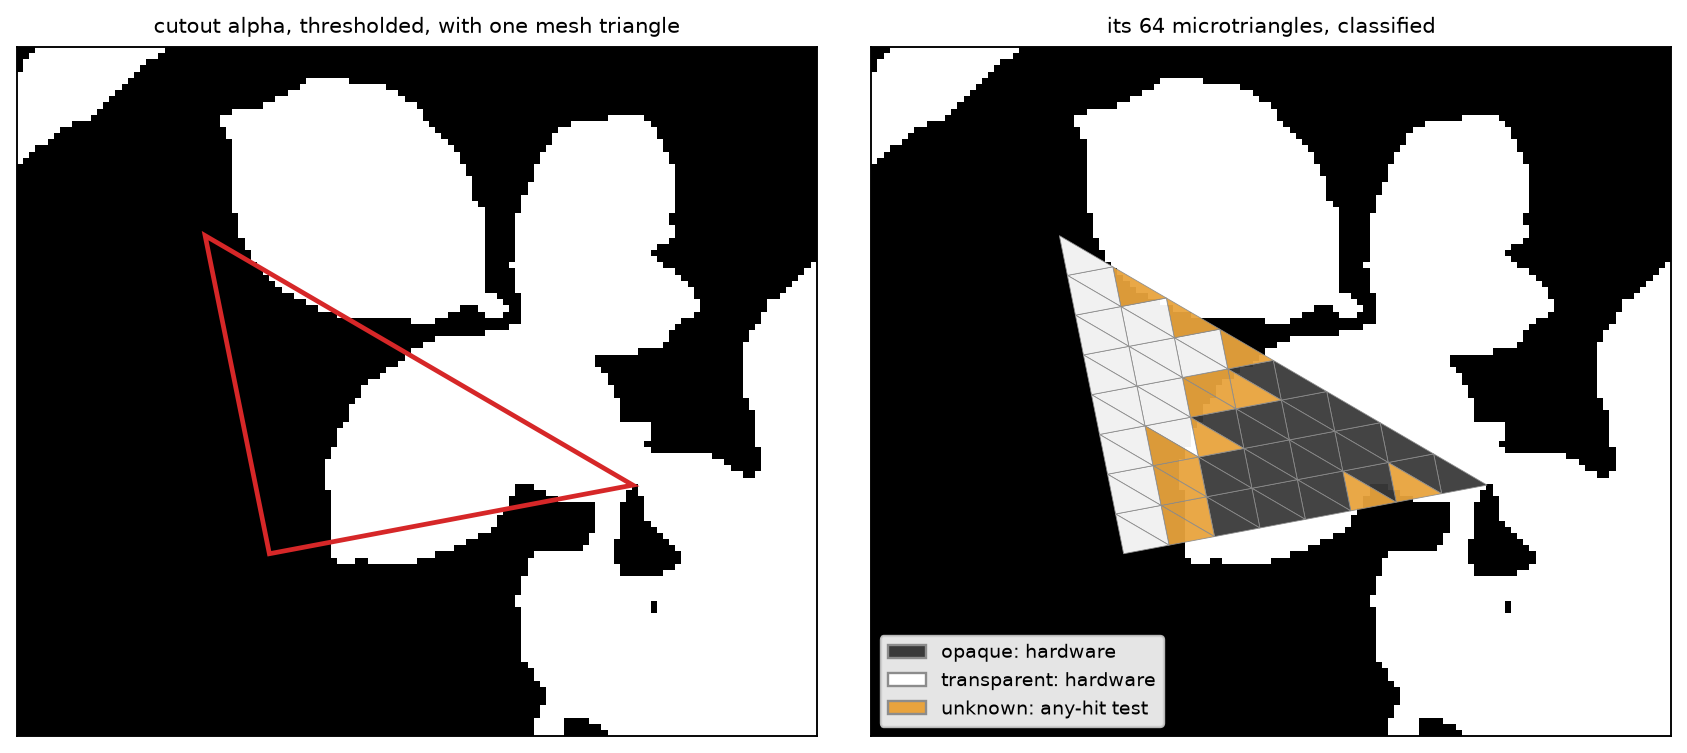
\includegraphics[width=\textwidth]{figures/omm_classify.png}
\caption[Klasifikacija opacity micromap-a ise\v{c}enog trougla]{\v{S}ta pe\v{c}enje proizvodi, za jedan stvarni trougao Sponza materijala sa isecanjem, na isporu\v{c}enom nivou podele. \textbf{Levo:} alfa materijala pragovana na svojoj granici, belo gde zrak poga\dj{}a i crno gde prolazi, sa ocrtanim trouglom. \textbf{Desno:} njegovih \ommTotal{} mikrotrouglova, svaki klasifikovan prema uzorcima u njemu. Samo \ommUnknown{} preseca alfa granicu i ostaje nepoznato, pa je \ommHwPct\% trougla razre\v{s}eno tokom obilaska, a any-hit alfa test radi samo na narand\v{z}astom pojasu. Mikrotrougao se naziva neprozirnim ili prozirnim samo kad se svi uzorci u njemu sla\v{z}u, pa nejasan uvek pada na ta\v{c}an test, te ekstenzija menja cenu obilaska, a ne ono \v{s}to on nalazi.}
\label{fig:omm}
\end{figure}

Engine uklju\v{c}uje \texttt{VK_KHR_ray_query} i \texttt{VK_KHR_acceleration_structure} (plus \texttt{VK_KHR_deferred_host_operations} za izgradnju), ali ne i ekstenziju ray tracing pipeline-a. Ne postoji shader binding table: svako pra\'cenje je \texttt{RayQuery} objekat kreiran unutar ina\v{c}e obi\v{c}nog compute ili fragment \v{s}ejdera.

Tamo gde bi DXR slao hit grupu po geometriji, ovde se ni\v{s}ta ne \v{s}alje: \v{s}ejder dobija tri celobrojne vrednosti i sam mora da prona\dj{}e povr\v{s}inu, vode\'ci indeks instance kroz \texttt{GeoRecord} tabelu na adresi ure\dj{}aja do bafera indeksa i temena mesha i njegovog bindless materijala (Slika~\ref{fig:hitresolve}). Jedna rutina, \texttt{ResolveHit} u \texttt{RTHitShading.hlsli}, stoga razre\v{s}ava \emph{bilo koji} mesh u sceni bez \v{s}ejdera po geometriji i bez ponovnog vezivanja deskriptora, \v{s}to i omogu\'cava da se jedan \texttt{ShadeSurfaceHit} koristi iz sva \v{c}etiri efekta.

\begin{figure}[tbp]
\centering
\begin{tikzpicture}[>={Stealth[]}, font=\small, node distance=4mm,
  box/.style={draw, rounded corners, align=left, inner sep=4pt, text width=4.4cm},
  src/.style={box, fill=black!7}]
  \node[src] (hit) {\textbf{Pogo\dj{}eni trougao}\\\footnotesize \texttt{instanceId}, \texttt{prim},
    \texttt{bary}};
  \node[box, below=8mm of hit] (rec) {\textbf{\texttt{GeoRecord}}\\\footnotesize adrese bafera temena i indeksa, indeks teksture, materijal};
  \node[box, right=16mm of rec] (idx) {\textbf{Bafer indeksa}\\\footnotesize tri indeksa na
    \texttt{IndexAddress + prim*12}};
  \node[box, below=8mm of rec] (vtx) {\textbf{Bafer temena}\\\footnotesize atributi, interpolirani
    barycentrics-ima};
  \node[box, right=16mm of vtx] (tex) {\textbf{Bindless niz tekstura}\\\footnotesize
    \texttt{NonUniformResourceIndex}};
  \node[src, below=8mm of vtx] (out) {\textbf{\texttt{HitSurface}}\\\footnotesize albedo, normala,
    metalnost, hrapavost};
  \draw[->] (hit) -- node[right, font=\scriptsize] {tabela preko adrese} (rec);
  \draw[->] (rec) -- (idx);
  \draw[->] (rec) -- (vtx);
  \draw[->] (idx) -- (vtx);
  \draw[->] (rec.east) to[out=-30, in=30] (tex.north east);
  \draw[->] (tex) -- (out);
  \draw[->] (vtx) -- (out);
\end{tikzpicture}
\caption[Razre\v{s}avanje pogotka kroz bindless tabelu geometrije]{Od pogo\dj{}enog trougla do osen\v{c}ene povr\v{s}ine, bez shader binding table-a. \texttt{RayQuery} vra\'ca samo tri broja, a iz njih \texttt{ResolveHit} sti\v{z}e do geometrije i materijala kroz tabelu indeksiranu preko \texttt{instanceCustomIndex}. Indeks teksture nije uniforman unutar wave-a, pa mora da pro\dj{}e kroz \texttt{NonUniformResourceIndex}.}
\label{fig:hitresolve}
\end{figure}

\section{\v{C}etiri efekta preko inline ray query-ja}
\label{sec:efekti}

Sva \v{c}etiri efekta dele istu osnovnu operaciju: konstruisati zrak, kreirati \texttt{RayQuery} nad TLAS-om scene, izvr\v{s}iti njegovu petlju obilaska i postupiti prema rezultatu. Razlikuju se po \v{c}etiri ose iz Tabele~\ref{tab:effect-params}, od kojih su dve spregnute: efekat kome treba samo odgovor o vidljivosti mo\v{z}e da stane na prvom pogotku, \v{s}to je i jeftiniji obilazak i razlog za\v{s}to mo\v{z}e da priu\v{s}ti manji broj zraka od efekta koji mora da osen\v{c}i ono \v{s}to na\dj{}e.

\begin{table}[tbp]
\caption[Parametri \v{c}etiri efekta]{Kako se \v{c}etiri efekta razlikuju pod istom inline ray query operacijom. Broj zraka i razmera su podrazumevane vrednosti odgovaraju\'cih CVar-ova. ``Prvi pogodak'' je \texttt{RAY\_FLAG\_ACCEPT\_FIRST\_HIT\_AND\_END\_SEARCH}, koji zaustavlja obilazak \v{c}im na\dj{}e bilo kakav presek.}
\label{tab:effect-params}
\centering
\begin{tabular}{lllll}
\toprule
Efekat & zraka/piksel & obilazak & rezultat pogotka & razmera \\
\midrule
senke        & 2 po svetlu & prvi pogodak & vidljivost (0/1)  & 1.0 \\
AO           & 2           & prvi pogodak & okluzija + rastojanje & 0.5 \\
refleksije   & 1           & najbli\v{z}i     & osen\v{c}ena radijansa   & 1.0 \\
GI           & 2           & najbli\v{z}i     & osen\v{c}ena radijansa   & 0.5 \\
\bottomrule
\end{tabular}
\end{table}

Efekti koji \v{s}ejdiraju svoje pogotke (refleksije i GI) dele jednu rutinu, \texttt{ShadeSurfaceHit} u \texttt{RTHitShading.hlsli}, koja razre\v{s}ava pogo\dj{}eni trougao kroz bindless tabelu geometrije i ra\v{c}una jedan odskok, dok senkama i AO treba samo odgovor o vidljivosti i koriste jeftiniji any-hit obilazak. Primarno \v{s}ejdiranje u forward prolazu je standardni metallic-roughness Cook-Torrance model (GGX distribucija, Smith geometrija sa Schlick-GGX aproksimacijom, Schlick Fresnel, Lambertov difuzni \v{c}lan), sa ambijentalnim \v{c}lanom iz prefiltriranog cube mape okru\v{z}enja i unapred izra\v{c}unate tabele BRDF-a.

Sekundarni pogoci se \v{s}ejdiraju jeftinije, namerno: \texttt{ShadeSurfaceHit} ra\v{c}una Lambertov difuzni \v{c}lan skaliran sa $(1 - \text{metallic})$, plus emisivni \v{c}lan povr\v{s}ine i image-based ambijentalno punjenje, bez ikakvog spekularnog re\v{z}nja, pa provodnik vi\dj{}en u refleksiji ili kroz GI odskok vra\'ca crno umesto ogledalskog odsjaja. Spekularni odsjaj drugog odskoka je redak i niskog kontrasta kad ga denoiser konvoluira, dok bi puna evaluacija BRDF-a u svakom pogotku otprilike udvostru\v{c}ila cenu putanje \v{s}ejdiranja pogotka. Cena aproksimacije je odsustvo me\dj{}urefleksije metala o metal, koju path tracer iz Odeljka~\ref{sec:pathtracer} reprodukuje, pa se ona pojavljuje kao mala sistematska razlika u metrikama refleksija.

Za evaluaciju u Glavi~\ref{ch:analiza}, ambijentalna okluzija, refleksije i globalno osvetljenje mogu se proizvesti i screen-space aproksimacijom, biranom preko pode\v{s}avanja moda (\texttt{render.ao.mode}, \texttt{render.reflections.mode}, \texttt{render.gi.mode}). SSAO, SSR i SSGI \v{c}itaju isti G-bafer dubine i normala i pi\v{s}u u isti slot kao njihov parnjak sa pra\'cenjem zraka (SSGI mar\v{s}iranjem po baferu dubine puni isti GI cilj u polovini rezolucije, pa te\v{c}e kroz isti temporalni/denoise/upsample/forward rep), te se dve verzije datog efekta razlikuju samo po na\v{c}inu na koji se signal proizvodi. One su osnovne linije iz Odeljka~\ref{sec:poredjenje}. Gather za SSGI nema proveru podr\v{s}ke ure\dj{}aja i radi na bilo kom GPU-u, dok je GI sa pra\'cenjem zraka (mod 2) onaj koji se bez podr\v{s}ke za ray tracing gasi.

\subsection{Senke (RT senke)}
\label{sec:senke}

Senke se prate inline u forward prolazu, jednom po svetlu po pikselu za svako uklju\v{c}eno usmereno, ta\v{c}kasto i spot svetlo (do \v{c}etiri usmerena), u punoj rezoluciji i bez denoisera izme\dj{}u (\texttt{DefaultLit.frag.hlsl} i zajedni\v{c}ki RT include-i, u \texttt{SS_RAYTRACING} permutaciji). Zrak senke je \v{c}ist test vidljivosti, pa koristi najjeftiniji obilazak, \texttt{ACCEPT_FIRST_HIT_AND_END_SEARCH}. Taj obilazak nije potpuno fiksne funkcije, jer se geometrija sa isecanjem mora razre\v{s}iti u \v{s}ejderu: kandidati pogodaka na trouglovima koji nisu neprozirni vra\'caju se kroz \texttt{q.Proceed()}, gde se testira alfa materijala i pogodak potvr\dj{}uje samo ako pro\dj{}e, a prvi pre\v{z}iveli pogodak ozna\v{c}ava povr\v{s}inu kao u senci. Po\v{c}etak zraka pomeren je du\v{z} normale povr\v{s}ine i ka svetlu (\texttt{positionWS + Ng*0.02 + L*0.01}) da bi se izbeglo samopresecanje (Listing~\ref{lst:shadow}). Pomeraj koristi normalu \v{s}ejdiranja koju je forward prolaz ve\'c razre\v{s}io, a to je ono \v{s}to mesto poziva prosle\dj{}uje uprkos imenu parametra.

Alternativa koju engine zadr\v{z}ava je rasterska shadow mapa, ujedno podrazumevana i rezerva na ure\dj{}aju bez ray tracing-a (Slika~\ref{fig:shadow-vs-map}). Sunce zadr\v{z}ava posebnu mapu, a \texttt{render.shadow.directionals} (podrazumevano 1) dozvoljava do tri dodatna usmerena svetla da dele atlas plo\v{c}ica prilago\dj{}enih sceni, od kojih svaka ko\v{s}ta jo\v{s} jedan prolaz dubine scene, dok putanja sa pra\'cenjem zraka ignori\v{s}e taj bud\v{z}et i prati svako usmereno svetlo koje baca senku. Materijali sa isecanjem (alfa maska) renderuju se u mapu kroz poseban \texttt{ShadowMasked} pipeline koji testira alfu materijala. Presecanje prave geometrije ne tra\v{z}i nikakvo pode\v{s}avanje depth bias-a, iako njegova cena raste sa brojem svetala, dok se mapa amortizuje na ceo frejm. Odeljak~\ref{sec:analiza-shadow-strategy} meri taj kompromis. Sekundarna usmerena svetla samo osvetljavaju i zasen\v{c}avaju scenu: GI, refleksije, path tracer, disk neba i image-based ambijent \v{c}itaju samo prvo svetlo.

\begin{figure}[tbp]
\centering
\begin{minipage}{0.48\textwidth}\centering
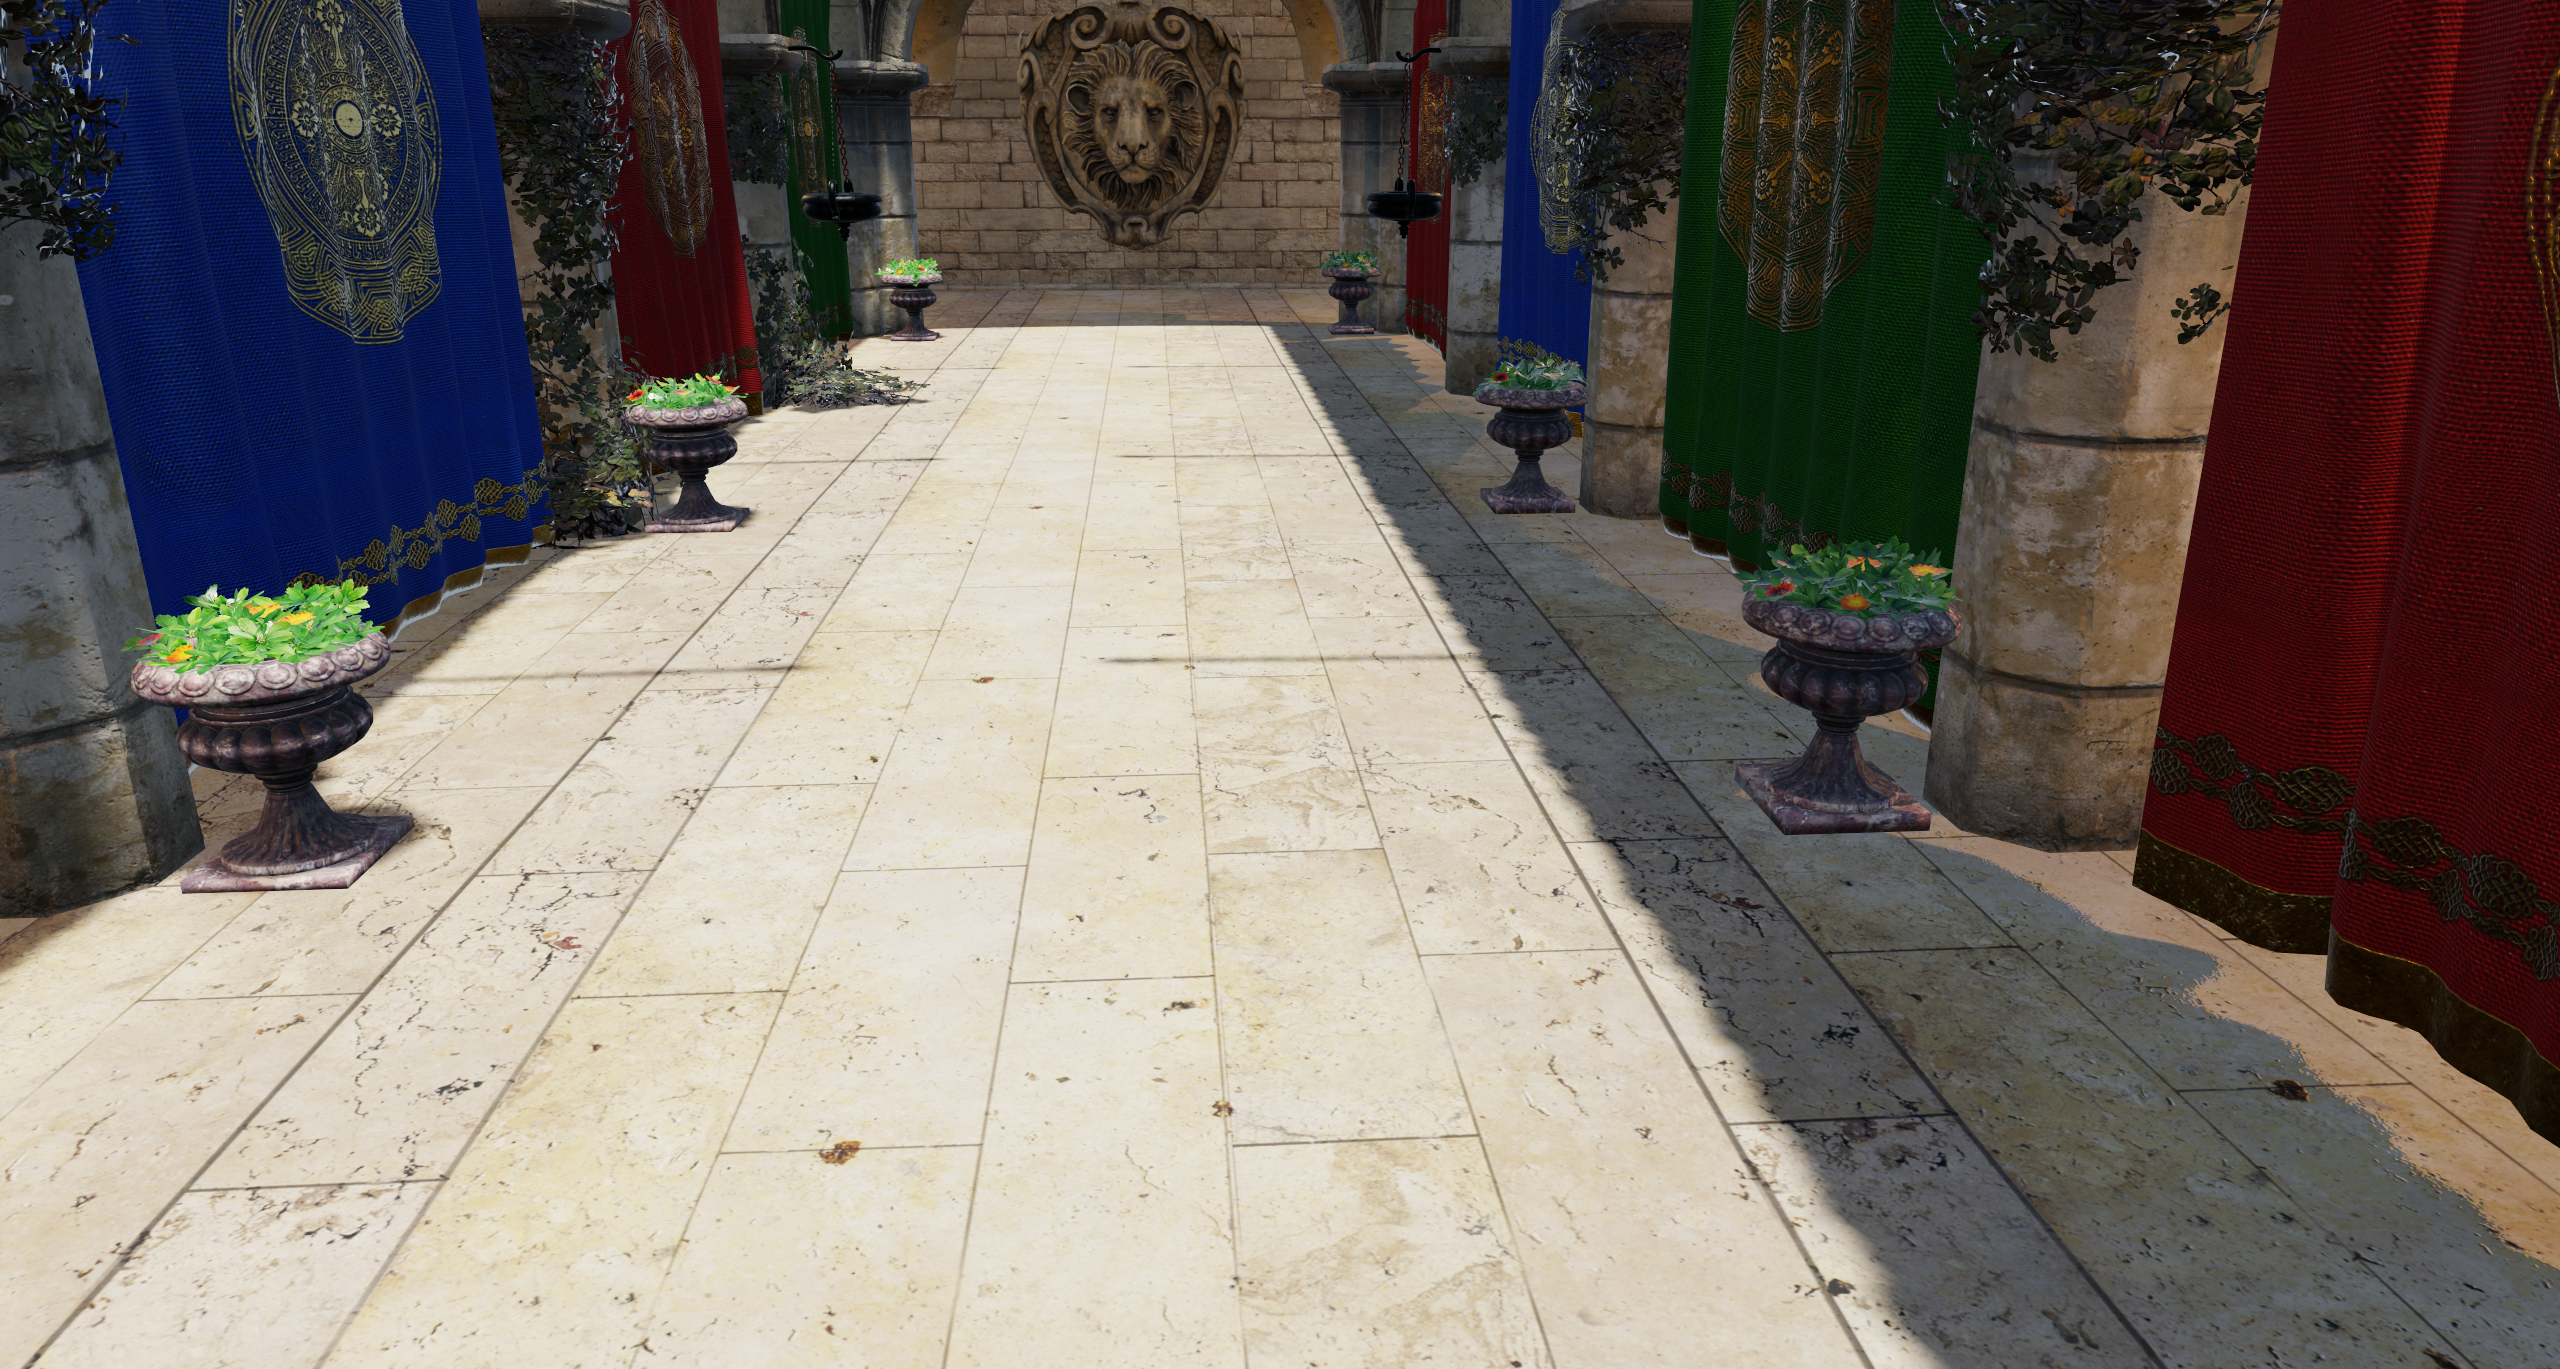
\includegraphics[width=\linewidth]{figures/shadow_map.png}\\{\small shadow mapa (raster)}
\end{minipage}\hfill
\begin{minipage}{0.48\textwidth}\centering
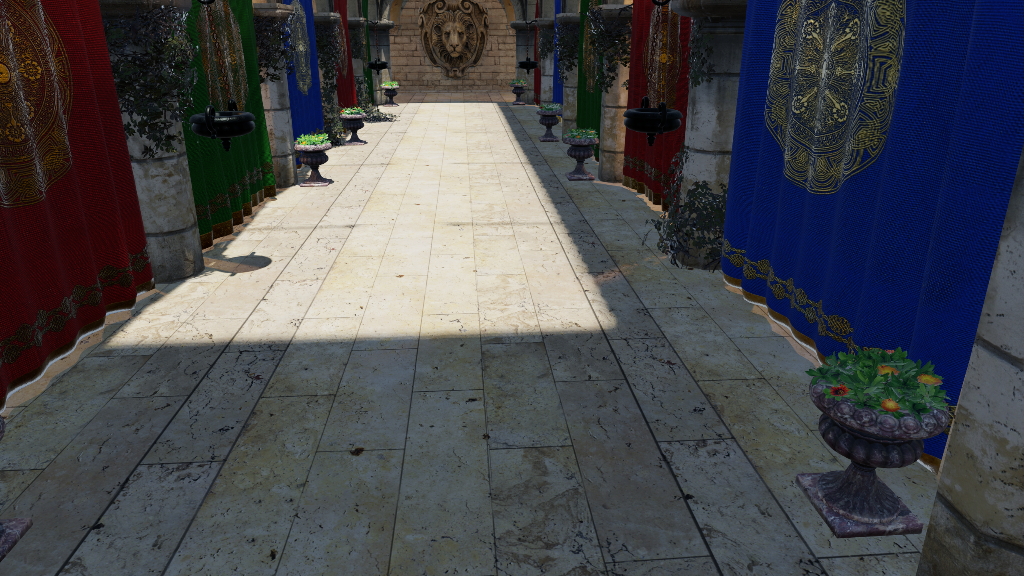
\includegraphics[width=\linewidth]{figures/shadow_rt.png}\\{\small senke pra\'cenjem zraka}
\end{minipage}
\caption[Shadow mapa naspram senki pra\'cenjem zraka]{Ista poza i isto svetlo, \texttt{render.shadows.mode} 1 naspram 2. Urne na osun\v{c}anom podu su mesto na koje treba gledati: rasterska mapa ima kona\v{c}nu rezoluciju i depth bias, pa se njihove kontaktne senke odvajaju od podno\v{z}ja i razmazuju, dok ih pra\'cena verzija usidrava uz pravu geometriju. Snimci su deterministi\v{c}ki (dva uzastopna snimka jedne konfiguracije su bit-identi\v{c}na), pa je svaka razlika izme\dj{}u panela stvarna.}
\label{fig:shadow-vs-map}
\end{figure}


\needspace{22\baselineskip}
\begin{lstlisting}[caption={Inline ray query test vidljivosti za senku (HLSL).}, label={lst:shadow}]
RayQuery<RAY_FLAG_ACCEPT_FIRST_HIT_AND_END_SEARCH> q;
RayDesc ray;
ray.Origin    = positionWS + Ng * 0.02 + L * 0.01;
ray.Direction = L;
ray.TMin      = 0.0;
ray.TMax      = distanceToLight - 0.05;   // sun: effectively infinite
q.TraceRayInline(SceneTLAS, RAY_FLAG_NONE, 0xFF, ray);
while (q.Proceed())                       // alpha-test cutout candidates
{
    if (q.CandidateType() == CANDIDATE_NON_OPAQUE_TRIANGLE &&
        RTCommitCandidate(tableAddr, q.CandidateInstanceID(),
                          q.CandidatePrimitiveIndex(),
                          q.CandidateTriangleBarycentrics(), LinearSampler))
    {
        q.CommitNonOpaqueTriangleHit();
    }
}
bool shadowed = (q.CommittedStatus() == COMMITTED_TRIANGLE_HIT);
\end{lstlisting}

Preko CVar-a \texttt{render.shadow.soft} izlo\v{z}ena su dva nivoa kvaliteta. Tvrda putanja baca jedan zrak pravo ka svetlu, dok meka baca \texttt{SHADOW_RAY_COUNT = 2} zraka koji uzorkuju, uniformno po prostornom uglu, konus pod kojim izvor vidi osen\v{c}ena ta\v{c}ka (Slika~\ref{fig:shadow}), usrednjavaju\'ci pogotke u faktor penumbre u $[0,1]$. Poluugao prati izvor: polovina ugaonog pre\v{c}nika \texttt{render.shadow.sun\_angle\_deg} za sunce i $\arcsin(r/d)$ za lokalno svetlo polupre\v{c}nika \texttt{render.shadow.source\_radius} na rastojanju $d$, pa fizi\v{c}ki ve\'ci ili bli\v{z}i izvor daje mek\v{s}u ivicu. Uzorkovanje prostornog ugla umesto diska u tangentnoj ravni \v{c}ini da se penumbra u realnom vremenu sla\v{z}e sa next-event estimation-om path tracer-a pri bilo kojoj \v{s}irini konusa, a ne samo u granici malih uglova gde se dve parametrizacije poklapaju. \texttt{SHADOW_RAY_COUNT} je konstanta vremena kompajliranja, klasa cene, a ne podesivo dugme.

Pravci dolaze iz spatiotemporal blue noise-a \cite{wolfe2022stbn}, po dve dekorelisane dimenzije po svetlu, pa dvouzorkovnu penumbru raspore\dj{}uju po frejmovima da bi je temporalni akumulator razre\v{s}io (Odeljci~\ref{sec:denoising} i \ref{sec:taa}). Redosled je va\v{z}an iz dva razloga koje slika jednog frejma ne mo\v{z}e da poka\v{z}e: he\v{s} ponovo ba\v{c}en svakog frejma je beo u vremenu i akumulatoru ne ostavlja ni\v{s}ta \v{s}to bi usrednjio, a izvo\dj{}enje obe koordinate konusa iz jednog skalara uru\v{s}ava konus u krivu. Dimenzije po svetlu tako\dj{}e dekoreli\v{s}u svetla me\dj{}usobno, pa im gre\v{s}ka opada sa brojem svetala umesto da se poja\v{c}ava. Cena je \(+0.088\) ms na prolazu Forward, ispod praga materijalnosti iz Odeljka~\ref{sec:cena}.

\begin{figure}[tbp]
\centering
\begin{tikzpicture}[>={Stealth[]}]
  \draw[thick] (-2.6,0) -- (2.6,0);                      % surface
  % light-source disk (perpendicular to L), drawn as a circle
  \draw[fill=black!8] (2.7,2.4) circle (0.45);
  \node[font=\scriptsize, align=center] at (2.7,3.25) {izvor\\(polupre\v{c}nik $r$)};
  % direction to the light centre
  \draw[dashed] (0,0) -- (2.7,2.4);
  \node[font=\scriptsize] at (1.55,1.05) {$L$};
  % sample rays fanning to distinct points across the disk
  \draw[->, black!65] (0,0) -- (2.72,2.83);
  \draw[->, black!65] (0,0) -- (3.08,2.22);
  \draw[->, black!65] (0,0) -- (2.36,2.06);
  \draw[<->, black!45] (2.62,2.72) arc (46:38:3.6);
  \node[font=\scriptsize, black!55] at (3.02,2.52) {$\theta/2$};
  \fill (0,0) circle (1.7pt) node[below=3pt] {$P$};
\end{tikzpicture}
\caption[Uzorkovanje konusa meke senke]{Meke senke: iz ta\v{c}ke $P$ zraci se uzorkuju uniformno po prostornom uglu unutar konusa pod kojim izvor vidi oko pravca $L$, sa poluuglom $\theta/2$ odre\dj{}enim polupre\v{c}nikom izvora $r$ i rastojanjem. Udeo neblokiranih zraka daje penumbru.}
\label{fig:shadow}
\end{figure}

\v{S}irina penumbre je $2H\tan(\theta/2)$ po rastojanju okludera do prijemnika $H$ i ugaonoj veli\v{c}ini izvora $\theta$, zbog \v{c}ega Slika~\ref{fig:shadow-hs} kadrira osun\v{c}anu traku poda: sunce je jedino svetlo ovde sa udaljenim okluderom, dok se \v{c}etiri uklju\v{c}ene baklje nalaze na par jedinica od zidova koje osvetljavaju. \v{C}ak i tu pravi ugaoni pre\v{c}nik daje oko 36 piksela na snimku \v{s}irine 2560, pa ga slika preuveli\v{c}ava i to navodi.

Pogon suncem umesto preko \texttt{render.shadow.source\_radius} je namerna odluka, iz razloga koji je ujedno i ograni\v{c}enje. Uzorci konusa koji padaju ispod horizonta normale \v{s}ejdiranja preska\v{c}u se, a prosek se i dalje deli punim brojem uzoraka, \v{s}to je samo po sebi ispravno (njihovo ra\v{c}unanje kao osvetljenih je curenje koje next-event estimation u path tracer-u odbacuje), iako zna\v{c}i da \v{s}iri konus sistematski zatamnjuje povr\v{s}ine pod o\v{s}trim uglom. Pri polupre\v{c}niku od 1.5 jedinica to zatamnjenje \v{c}ini oko tri \v{c}etvrtine razlike me\dj{}u frejmovima i gu\v{s}i penumbru koju je trebalo da poka\v{z}e. Skoro vertikalno sunce to izbegava, jer poga\dj{}a pod tamo gde ni\v{s}ta nije odba\v{c}eno zbog horizonta.

\begin{figure}[tbp]
\centering
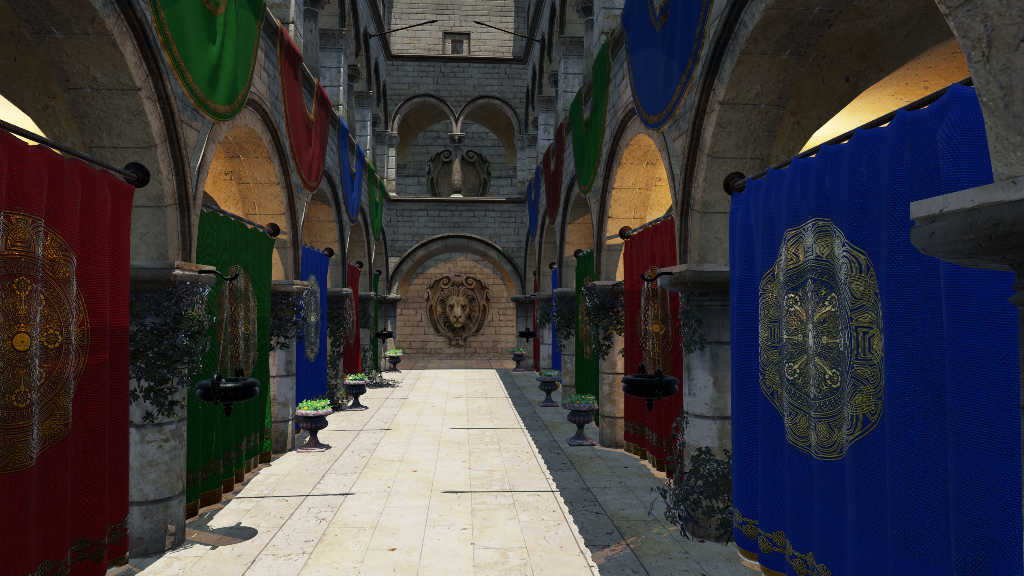
\includegraphics[width=0.48\textwidth]{figures/shadow_hard.png}\hfill%
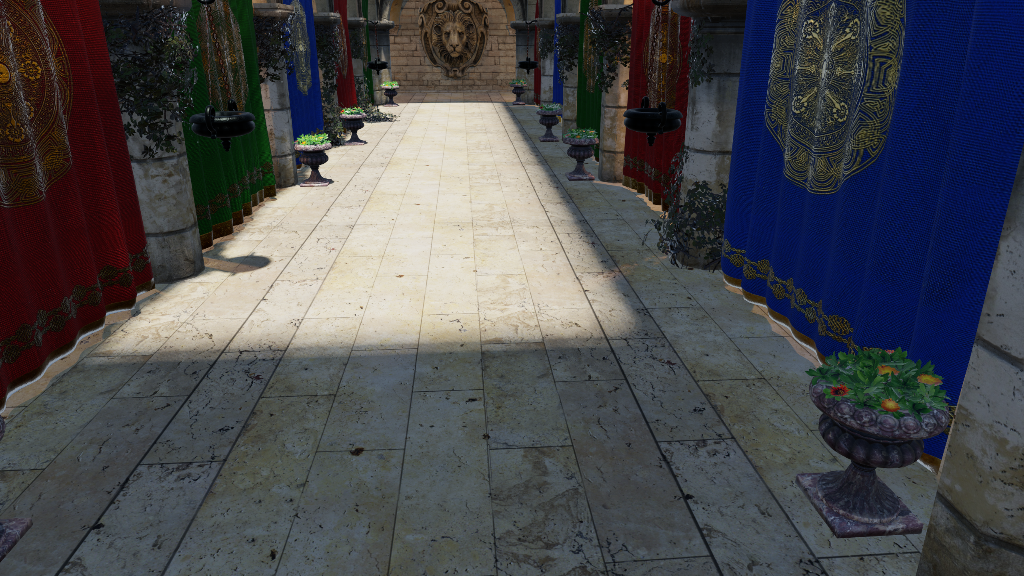
\includegraphics[width=0.48\textwidth]{figures/shadow_soft.png}
\caption[Tvrde naspram mekih senki pra\'cenjem zraka]{Tvrde (levo) naspram mekih (desno) senki pra\'cenjem zraka na osun\v{c}anoj traci poda, koje baca ivica krovnog svetlarnika oko 10.4 jedinica iznad nje: jedina razlika je \texttt{render.shadow.soft}. Ugaoni pre\v{c}nik sunca podignut je na $3^\circ$, oko \v{s}est puta fizi\v{c}kih $0.53^\circ$, jer je pri pravoj vrednosti penumbra u\v{z}a nego \v{s}to \v{s}tampa mo\v{z}e da razre\v{s}i. Treba \v{c}itati \v{s}irinu prelaza, a ne njegovu \v{c}isto\'cu: tvrda ivica nosi i detalj siluete ivice svetlarnika, koji penumbra usrednjava, pa se paneli razlikuju i u o\v{s}trini i u izlomljenosti istovremeno, a samo prva je predmet. Penumbra ovde ima otprilike konstantnu \v{s}irinu jer je baca jedan okluder na jednoj visini. \v{S}irenje sa rastojanjem okludera, re\v{c}itiji potpis povr\v{s}inskog izvora, zahtevalo bi senku koja putuje, a sa suncem na $80^\circ$ iznad horizonta ni\v{s}ta u ovoj sceni takvu ne baca.}
\label{fig:shadow-hs}
\end{figure}

\paragraph{Stohasti\v{c}ka alternativa.} Pra\'cenje svakog svetla u svakom pikselu je ta\v{c}no, ali raste linearno sa brojem svetala, \v{s}to ne pre\v{z}ivljava scenu osvetljenu stotinama izvora. Engine zato implementira drugu strategiju, uklju\v{c}enu preko \texttt{render.shadows.stochastic} i podrazumevano isklju\v{c}enu, prema MegaLights pristupu \cite{epic_megalights}: svaki piksel uzima \texttt{render.shadows.rays} nezavisnih uzoraka (ovaj CVar pokre\'ce samo ovu putanju, a ne inline gore, \v{c}iji je broj zraka konstanta vremena kompajliranja), a svaki uzorak zasebno koristi resampled importance sampling \cite{talbot2005ris} da izabere \emph{jedno} svetlo sa verovatno\'com proporcionalnom njegovom nezasen\v{c}enom doprinosu i prati jedan zrak ka njemu. Usrednjavanje uzoraka daje jedan agregatni odnos vidljivosti, pa cenu odre\dj{}uje broj uzoraka, a ne broj svetala. Procena je nepristrasna, ali izuzetno \v{s}umovita, jer uzorci jednog piksela ne govore ni\v{s}ta o tome koja je svetla izvukao njegov sused, pa ova putanja nu\v{z}no radi kao poseban lanac u polovini rezolucije, \texttt{RTShadow} $\rightarrow$ \texttt{ShadowTemporal} $\rightarrow$ \texttt{ShadowDenoise0..2} $\rightarrow$ \texttt{ShadowUpsample}, koji ponovo koristi zajedni\v{c}ki denoiser, uz paralelni lanac demodulisanog spekulara za \v{c}lan spekularne okluzije. Ti prolazi nose sopstvene GPU timestamp opsege, koje Odeljak~\ref{sec:cena} obra\v{c}unava odvojeno od forward prolaza. Njena cena je konstantna po broju svetala, \v{s}to je ceo smisao: inline putanja pobe\dj{}uje za mali broj svetala, a gubi za mnogo. Odeljak~\ref{sec:analiza-shadow-strategy} meri ta\v{c}ku preseka na ovoj sceni, a debug prikazi izla\v{z}u agregatni bafer vidljivosti pre i posle filtriranja (Slika~\ref{fig:shadow-denoise-ab}), gde toliko malo uzoraka po pikselu ostavlja sirov odnos skoro binarnim \v{s}umom.

Podrazumevano je isklju\v{c}ena, a razlog je kompromis koji rekonstrukcija trenutno ne mo\v{z}e da razre\v{s}i. Njena procena po frejmu je bimodalna, ili nula ili redak svetao pik, zavisno od toga koje je svetlo piksel ponovo uzorkovao, a clamp boje u susedstvu, koji uklanja duhove na pokretnim ivicama iz GI i refleksija, pogre\v{s}an je za signal takvog oblika: gde se dva svetla preklapaju, lokalni opseg je uzak i taman, pa clamp dr\v{z}i akumuliranu istoriju dole i ostavlja crni \v{s}av izme\dj{}u dva svetla koji nikakvo filtriranje ne popunjava. Isklju\v{c}ivanje clamp-a tu, \v{s}to je isporu\v{c}eno pode\v{s}avanje, uklanja \v{s}av i vra\'ca razmazivanje pri kretanju kamere koje je clamp trebalo da spre\v{c}i. Oba izbora ostavljaju vidljiv defekt, pa inline ostaje podr\v{z}ana putanja.

Merenja se ne protive ni\v{c}emu od toga, a jedno od njih aktivno pokazuje pogre\v{s}nim smerom. Na ruti sa kretanjem stohasti\v{c}ka putanja je temporalno stabilnija od dve, tFLIP \mMegalightsTflip{} naspram \mRtShadowTflip{} inline-a, a Odeljak~\ref{sec:analiza-shadow-strategy} nalazi da je jeftinija od dve na RX 9070 XT. Ocenu stabilnosti treba \v{c}itati uz razmazivanje, a ne protiv njega: mera toga koliko se rezultat malo menja izme\dj{}u frejmova ne mo\v{z}e da razdvoji stabilno od razmazanog, \v{s}to Odeljak~\ref{sec:motion} obra\dj{}uje sa ovim parom kao radnim primerom. \v{S}av izmi\v{c}e merenju iz prozai\v{c}nijeg razloga, jer ruta nikad ne kadrira osvetljene bo\v{c}ne prolaze gde se dve baklje preklapaju. Podrazumevana vrednost je dakle postavljena uprkos metrikama, a ne prema njima, \v{s}to vredi otvoreno re\'ci u radu koji se ina\v{c}e oslanja na merenje.

\begin{figure}[tbp]
\centering
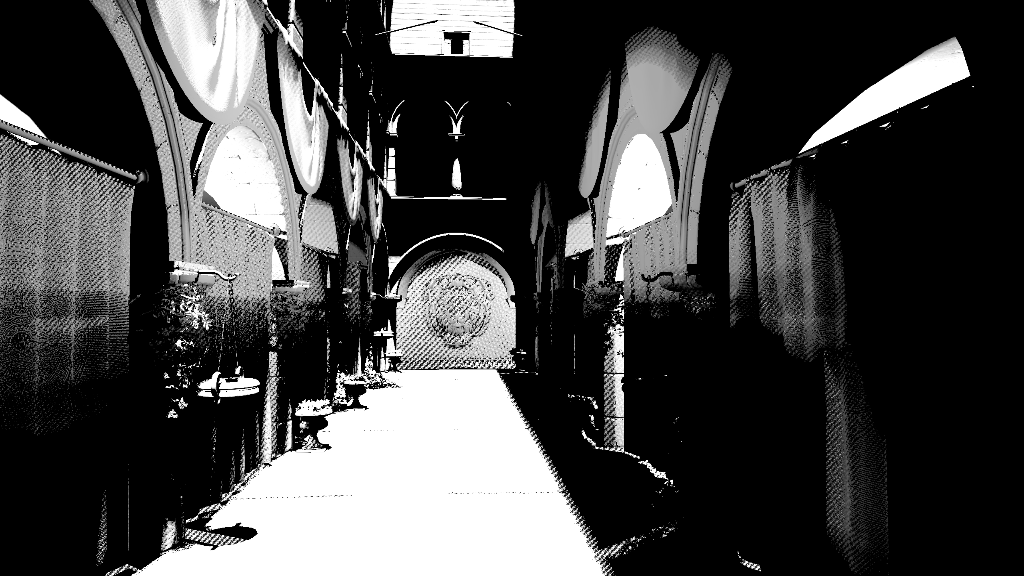
\includegraphics[width=0.48\textwidth]{figures/dbg_shadow_raw.png}\hfill%
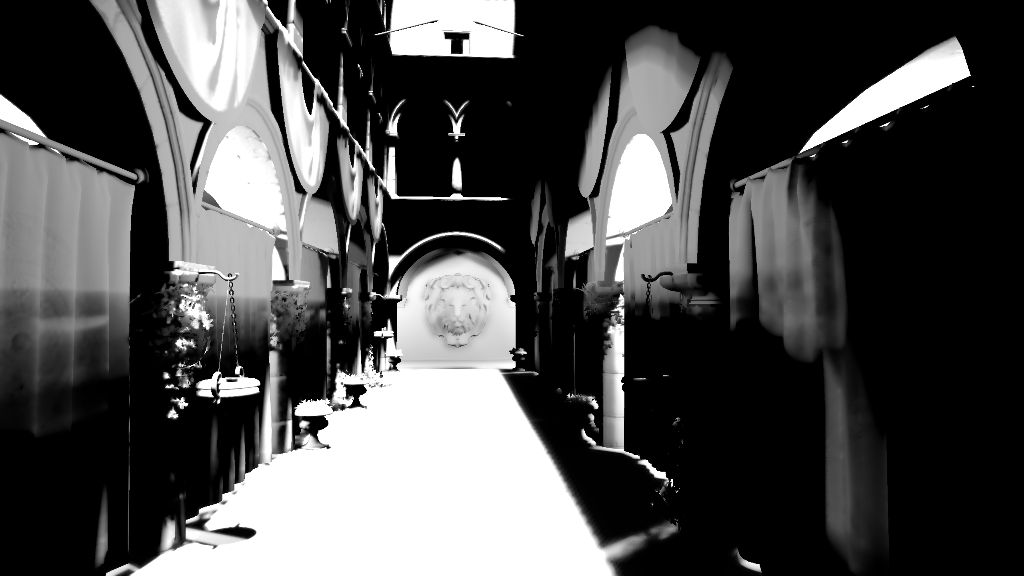
\includegraphics[width=0.48\textwidth]{figures/dbg_shadow_denoised.png}
\caption[Stohasti\v{c}ka vidljivost pre i posle denoising-a]{Stohasti\v{c}ki agregatni odnos vidljivosti pre (levo) i posle (desno) temporalne akumulacije i a-trous filtera (\texttt{render.debugview} 8 i 9). Belo je potpuno osvetljeno, crno potpuno u senci. Levi panel pokazuje koliko je sirov odnos po pikselu skoro binaran pri ovom broju uzoraka.}
\label{fig:shadow-denoise-ab}
\end{figure}

\subsection{Ambijentalna okluzija (AO)}

Ambijentalna okluzija je compute prolaz (\texttt{AO.comp.hlsl}) u polovini rezolucije. Svaki piksel rekonstrui\v{s}e svetsku poziciju iz G-bafera dubine i baca \texttt{render.ao.rays} kratkih zraka (podrazumevano 2, ograni\v{c}eno na $[1,16]$) po hemisferi sa kosinusnom te\v{z}inom oko geometrijske normale, rotiranoj po pikselu interleaved gradient noise-om, koriste\'ci isti \texttt{ACCEPT_FIRST_HIT_AND_END_SEARCH} obilazak vidljivosti kao senke. Zraci su ograni\v{c}eni na \texttt{render.ao.radius}, a pogodak doprinosi \texttt{1 - saturate(t / AORadius)}, pa bli\v{z}i okluderi zatamnjuju vi\v{s}e, a rezultat se skalira sa \texttt{render.ao.intensity} (Listing~\ref{lst:ao}). Slika~\ref{fig:ao-composited} pokazuje \v{s}ta to doprinosi gotovoj slici, a Slika~\ref{fig:ssvsrt-ao} pokazuje sam \v{c}lan naspram screen-space alternative.

\begin{figure}[tbp]
\centering
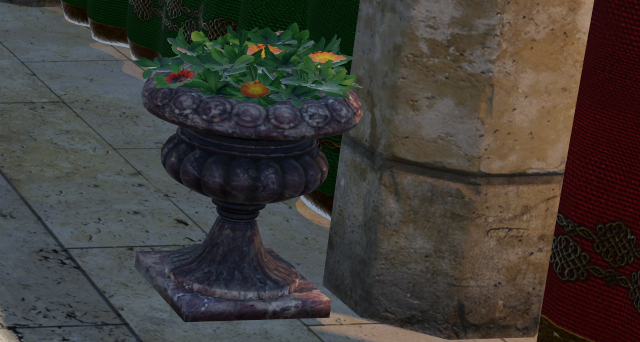
\includegraphics[width=0.485\textwidth]{figures/ao_off.png}\hfill
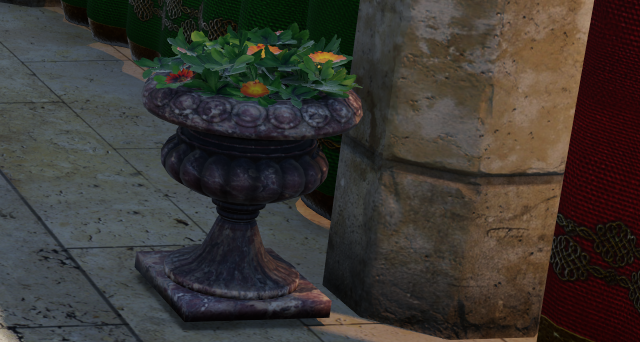
\includegraphics[width=0.485\textwidth]{figures/ao_on.png}
\caption[Ambijentalna okluzija u kompozitnom frejmu]{Ambijentalna okluzija isklju\v{c}ena (levo) i uklju\v{c}ena (desno), u gotovom frejmu a ne u AO baferu. Ovo je ise\v{c}ak, namerno: okluzija nastaje tamo gde geometrija obuhvata geometriju, pa je preko celog frejma efekat vredan 2.4 nivoa od 255 i neise\v{c}en par bi se \v{s}tampao kao dve identi\v{c}ne slike. Ovde je 6.2, a dobija se postolje usa\dj{}eno u pod umesto da lebdi nad njim, dubina izme\dj{}u listova i stub koji dodiruje tlo umesto da kroz njega prolazi. Odeljak~\ref{sec:poredjenje} je isto zapa\v{z}anje kao broj: AO ostavlja netaknuto pet \v{s}estina ovog frejma.}
\label{fig:ao-composited}
\end{figure}


\needspace{17\baselineskip}
\begin{lstlisting}[caption={Uzorkovanje hemisfere za AO (HLSL, reprezentativan ise\v{c}ak).}, label={lst:ao}]
float occlusion = 0.0;
for (uint k = 0; k < RayCount; ++k)
{
    float3 dir = CosineHemisphere(k, RayCount, ign, N); // cosine-weighted, IGN-rotated around N
    RayQuery<RAY_FLAG_ACCEPT_FIRST_HIT_AND_END_SEARCH> q;
    RayDesc ray = MakeRay(positionWS + N * 0.02, dir, 0.0, AORadius);
    q.TraceRayInline(SceneTLAS, RAY_FLAG_NONE, 0xFF, ray);
    while (q.Proceed()) { /* alpha-test cutout candidates, as in Listing 3.1 */ }
    if (q.CommittedStatus() == COMMITTED_TRIANGLE_HIT)
        occlusion += 1.0 - saturate(q.CommittedRayT() / AORadius);
}
occlusion = 1.0 - occlusion / RayCount;
\end{lstlisting}

Prolaz pi\v{s}e \texttt{float4(ao, ao, ao, meanHitT)}, pri \v{c}emu alfa kanal nosi srednje rastojanje do okludera. Taj alfa napaja \v{c}lan zaustavljanja ivica vo\dj{}en rastojanjem pogotka u denoiser-u (Odeljak~\ref{sec:denoising}), istu ideju koju NVIDIA-in ReBLUR denoiser \cite{nvidia_nrd} koristi da skalira prostorni filter prema tome koliko je okluder bio daleko. \v{C}lan je implementiran, ali podrazumevano isklju\v{c}en na svakom signalu, uklju\v{c}uju\'ci AO: pri dva zraka po pikselu rastojanje pogotka je previ\v{s}e \v{s}umovito da bi usmeravalo filter, a pogre\v{s}no usmeravanje je gore od nikakvog. Rezultat u polovini rezolucije se denoisuje i bilateralno upsample-uje pre nego \v{s}to ga forward prolaz pomno\v{z}i u ambijentalni \v{c}lan (Slika~\ref{fig:ao}).

\begin{figure}[tbp]
\centering
\begin{tikzpicture}[>={Stealth[]}]
  \draw[thick] (-2.7,0) -- (2.7,0);
  \draw[dashed] (-1.9,0) arc (180:0:1.9);
  \draw[->, thick] (0,0) -- (0,2.25) node[above] {$N$};
  \foreach \a in {30,60,90,120,150} \draw[->, black!60] (0,0) -- (\a:1.9);
  \draw[fill=black!12] (0.85,0.55) rectangle (1.3,1.25);
  \draw[thin] (1.3,1.1) -- (2.05,1.6);
  \node[font=\scriptsize, anchor=west] at (2.05,1.6) {okluder};
  \fill (0,0) circle (1.7pt) node[below=3pt] {$P$};
\end{tikzpicture}
\caption[Uzorkovanje hemisfere za ambijentalnu okluziju]{Uzorkovanje hemisfere za AO: iz ta\v{c}ke $P$ baca se nekoliko kratkih zraka po hemisferi oko normale $N$. Udeo koji poga\dj{}a geometriju unutar zadatog polupre\v{c}nika daje okluziju.}
\label{fig:ao}
\end{figure}

\subsection{Refleksije}

Refleksije su compute prolaz (\texttt{Reflection.comp.hlsl}) u punoj rezoluciji, za razliku od GI i AO gather-a u polovini rezolucije, jer detalj refleksije zavisi od pogleda i ne podnosi zamu\'cenje koje unosi pra\'cenje u polovini rezolucije plus upsample. Pikseli \v{c}ija je hrapavost jednaka ili ve\'ca od \texttt{render.reflections.max\_roughness} (podrazumevano 0.8) preska\v{c}u se i zadr\v{z}avaju spekular iz prefiltriranog cube-a, pa udeo frejma koji se prati zavisi od me\v{s}avine materijala u sceni. Svaki preostali piksel rekonstrui\v{s}e svetsku poziciju i reflektuje vektor pogleda oko normale \v{s}ejdiranja sa normal mapom (\v{c}ita se iz zasebnog G-bafera normala \v{s}ejdiranja, a ne geometrijske normale, pa se normal mape ispravno ogledaju; pe\v{c}ene normal mape su BC5, koji \v{c}uva samo X i Y, pa Z rekonstrui\v{s}e \texttt{NormalEncode.hlsli}, a path tracer dekodira kroz istu funkciju). Treba mu najbli\v{z}i pogodak, pa za razliku od upita vidljivosti koristi obi\v{c}an \texttt{RayQuery<RAY_FLAG_NONE>} i izvr\v{s}ava obilazak do kraja.

Sjajne refleksije se aproksimiraju pomeranjem svakog zraka unutar konusa \v{c}iji poluugao raste sa hrapavo\v{s}\'cu povr\v{s}ine (\texttt{roughness * ReflConeScale}), usrednjeno preko \texttt{render.reflections.rays} (podrazumevano 1), dok se ogledalska povr\v{s}ina (\texttt{roughness == 0}) svodi na jedan o\v{s}tar zrak. Pogoci se \v{s}ejdiraju preko \texttt{ShadeSurfaceHit} (sun\v{c}evo osvetljenje sa sopstvenim zrakom senke, emisivni \v{c}lan pogo\dj{}ene povr\v{s}ine, image-based ambijent), a proma\v{s}aj uzorkuje prefiltrirani cube neba. Za razliku od GI prolaza ispod, refleksije ne uzorkuju lokalna ta\v{c}kasta i spot svetla scene u pogotku. Isti importance-sampled estimator lokalnih svetala izmeren je i ovde i nije pomerio nijednu metriku kvaliteta za dvostruku cenu GI strane, pa je potpuno izba\v{c}en iz ovog prolaza pri kompajliranju umesto da je ostavljen iza isklju\v{c}ene zastavice, po istom standardu dokaza pre svega koji podrazumevano isklju\v{c}uje gore navedeni vodi\v{c} rastojanja pogotka. Prolaz pi\v{s}e sirovu reflektovanu radijansu plus rastojanje pogotka, dok se Fresnelov \v{c}lan, te\v{z}injenje BRDF-om i \texttt{render.reflections.intensity} primenjuju naknadno u forward prolazu (Slika~\ref{fig:refl}).

\begin{figure}[tbp]
\centering
\begin{tikzpicture}[>={Stealth[]}]
  \draw[thick] (-2.7,0) -- (2.7,0);
  \draw[->, thick] (0,0) -- (0,2.2) node[above] {$N$};
  \draw[->, black!55] (-2.05,2.05) -- (0,0); \node[font=\scriptsize] at (-1.55,1.35) {$V$};
  \foreach \a in {50,62,74} \draw[->, black!65] (0,0) -- (\a:2.15);
  \draw[dashed] (0,0) -- (62:2.3) node[above right, font=\scriptsize] {$R$};
  \node[font=\scriptsize, align=center] at (2.0,1.05) {konus\\(hrapavost)};
  \fill (0,0) circle (1.7pt) node[below=3pt] {$P$};
\end{tikzpicture}
\caption[Reflektovani pravac i konus hrapavosti]{Refleksije: reflektovani pravac $R$ vektora pogleda $V$ oko normale $N$. Glatka povr\v{s}ina daje jedan o\v{s}tar zrak, a gruba uzorkuje konus oko $R$.}
\label{fig:refl}
\end{figure}

Slika~\ref{fig:refl-onoff} pokazuje doprinos prolaza. Variranje \texttt{render.reflections.cone\_scale} od 0 (\v{c}ist ogledalski zrak) do 3 menja gotov frejm u proseku samo za 0.16 nivoa od 255, preko \v{s}est isprobanih poza kamere, dok isto A/B, izmereno na baferu refleksija pre kompozicije, pomera 43.7 nivoa i spu\v{s}ta visokofrekventnu energiju bafera sa \hfConeSharp{} na \hfConeGlossy{}, \v{s}to je 275 puta vi\v{s}e signala nego \v{s}to pokazuje kompozitno pore\dj{}enje. Uzrok je to \v{s}to je refleksija mali aditivni \v{c}lan pored direktnog osvetljenja, pa ga kompozitna slika krije: \v{c}lan koji je mali u kona\v{c}noj slici i dalje mo\v{z}e biti ceo sadr\v{z}aj svog me\dj{}ubafera. Slika konusa (Slika~\ref{fig:refl-cone}) stoga koristi izolovani bafer, iz istog razloga iz kog to radi i galerija efekata u Odeljku~\ref{sec:cena}.

\begin{figure}[tbp]
\centering
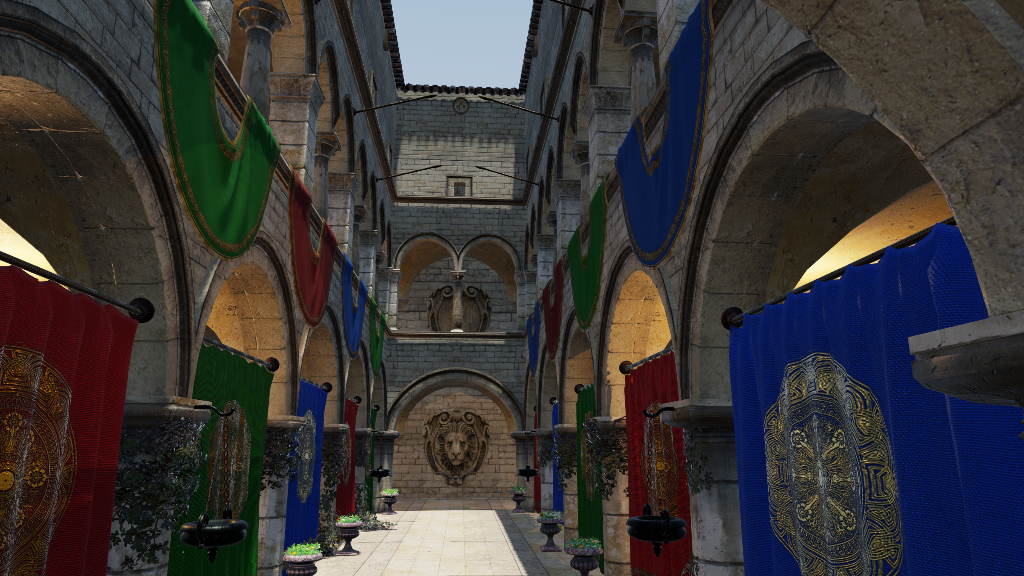
\includegraphics[width=0.48\textwidth]{figures/refl_off.png}\hfill%
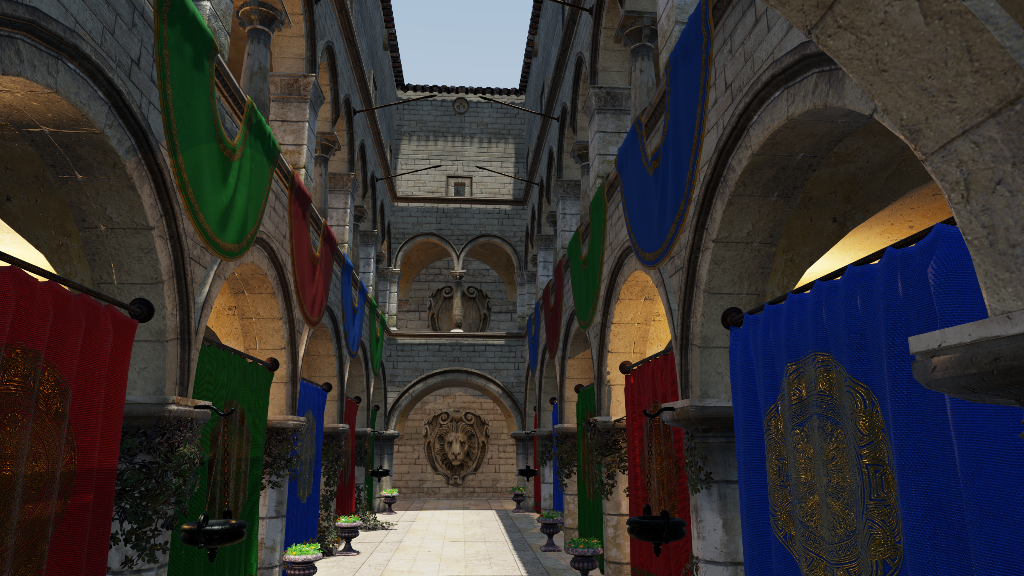
\includegraphics[width=0.48\textwidth]{figures/refl_rt.png}
\caption[Refleksije isklju\v{c}ene naspram refleksija pra\'cenjem zraka]{Bez refleksija (levo) naspram sa njima (desno), ise\v{c}eno na zlatni konac na draperiji pod uglom bliskim klize\'cem, gde je Fresnelov doprinos najve\'ci. Ise\v{c}eno iz istog razloga kao Slika~\ref{fig:ao-composited}: preko celog frejma prolaz vredi 3.3 nivoa od 255, a ovde 11.8. Dodaje se konac koji iz ravne boje prelazi u ne\v{s}to sa metalnim sjajem koji se menja dok se povr\v{s}ina okre\'ce. Vredi re\'ci \v{s}ta ova slika ne mo\v{z}e da poka\v{z}e, jer to ograni\v{c}ava efekat u ovoj sceni, a ne u tehnici: Sponza nema ogledalsku povr\v{s}inu, pa bafer refleksija vra\'ca ne\v{s}to spekulara od skoro svakog materijala, a prepoznatljivu reflektovanu sliku ni od jednog.}
\label{fig:refl-onoff}
\end{figure}

\begin{figure}[tbp]
\centering
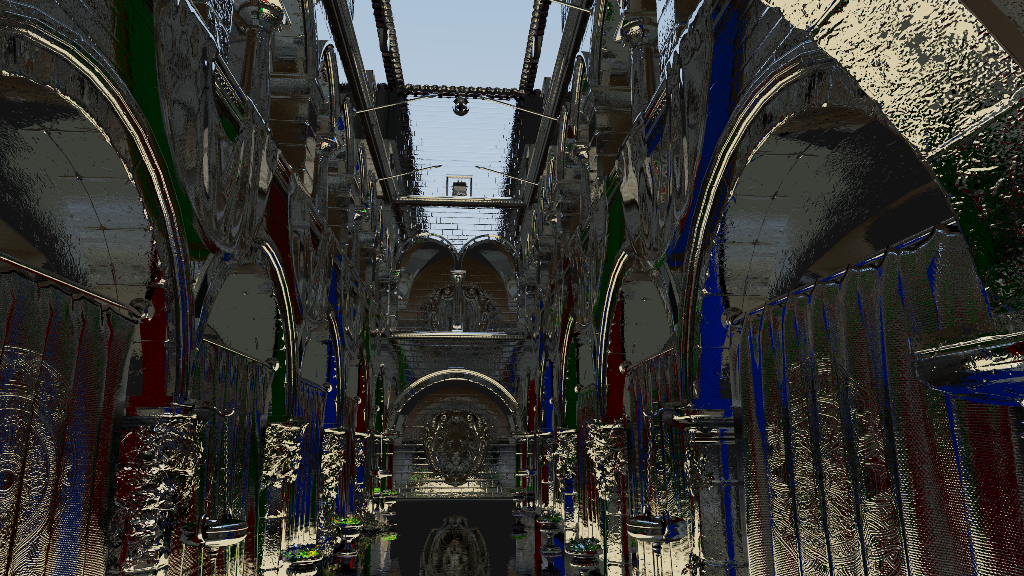
\includegraphics[width=0.48\textwidth]{figures/cone_sharp.png}\hfill%
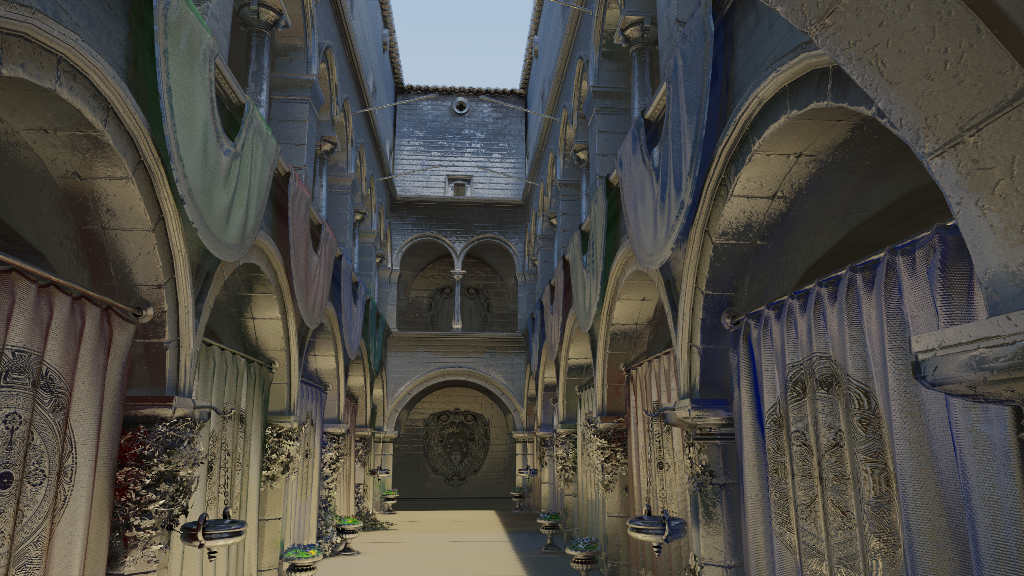
\includegraphics[width=0.48\textwidth]{figures/cone_glossy.png}
\caption[O\v{s}tar naspram sjajnog bafera refleksija]{Reflektovana radijansa pre kompozicije (\texttt{render.debugview} 3): o\v{s}tar ogledalski zrak, \texttt{cone\_scale} 0 (levo), naspram konusa pro\v{s}irenog hrapavo\v{s}\'cu, \texttt{cone\_scale} 3 (desno). Razlika je nevidljiva u gotovoj slici jer je refleksija mali aditivni \v{c}lan pored direktnog osvetljenja, iako je u sopstvenom baferu ceo sadr\v{z}aj.}
\label{fig:refl-cone}
\end{figure}

\subsection{Globalno osvetljenje (GI)}

Globalno osvetljenje je najskuplji efekat: compute prolaz (\texttt{GI.comp.hlsl}) u polovini rezolucije koji ra\v{c}una jedan odskok difuzne indirektne svetlosti. Hemisferu uzorkuje ta\v{c}no kao AO, \texttt{render.gi.rays} zraka (podrazumevano 2) do \texttt{render.gi.range}. Razlika je u onome \v{s}to zrak vra\'ca. Proma\v{s}aj uzorkuje cube neba, a svaki pogodak \v{s}ejdira \texttt{ShadeSurfaceHit}: sunce sa sopstvenim zrakom senke, emisivni \v{c}lan pogo\dj{}ene povr\v{s}ine, image-based ambijentalno punjenje i, kad je \texttt{render.rt.hit_lights} uklju\v{c}eno (podrazumevano), jedno od ta\v{c}kastih i spot svetala scene. To svetlo se bira importance sampling-om proporcionalno svom nezasen\v{c}enom doprinosu u pogotku i potvr\dj{}uje sopstvenim zrakom senke, kao nepristrasan estimator sa jednim uzorkom (isti koji koristi \texttt{RTShadowPass}, u duhu UE5 MegaLights) \v{c}ija je cena konstantna po broju svetala, za razliku od pune next-event estimation sume preko svih svetala, koja bi pomno\v{z}ila bud\v{z}et zraka u svakom sekundarnom pogotku. Ovaj \v{c}lan va\v{z}i samo za GI, a rutina ne prati dalje od ovih zraka senki, pa evaluacija ostaje jedan odskok.

Prolaz daje samo dolaznu iradijansu, bez albeda prijemnika, koji se mno\v{z}i u punoj rezoluciji u forward prolazu. To je konvencija demodulisane iradijanse na koju se oslanjaju i SVGF denoiser i probe sistemi poput DDGI/RTXGI \cite{majercik2019ddgi, nvidia_rtxgi}: filtriranje iradijanse umesto kona\v{c}ne boje spre\v{c}ava da detalj teksture albeda zavara zaustavljanje ivica denoisera. Forward prolaz zatim menja svoj ravni ambijentalni \v{c}lan ovim indirektnim osvetljenjem dobijenim pra\'cenjem zraka, istom zamenom koju prave Lumen i RTXGI \cite{epic_lumen}. Pri dva zraka po pikselu i polovini rezolucije (Slika~\ref{fig:gi}) sirov izlaz je upotrebljiv tek posle temporalnog-plus-prostornog denoise-a iz Odeljka~\ref{sec:denoising}.

\begin{figure}[tbp]
\centering
\begin{tikzpicture}[>={Stealth[]}]
  \draw[thick] (-2.9,0) -- (2.9,0);
  \draw[dashed] (-2.1,0) arc (180:0:2.1);
  \draw[->, thick] (0,0) -- (0,2.45) node[above] {$N$};
  \foreach \a in {35,70,110,145} \draw[->, black!60] (0,0) -- (\a:2.1);
  \foreach \a in {35,70,110,145} \fill[black!30] (\a:2.1) circle (2.4pt);
  \fill (0,0) circle (1.7pt) node[below=3pt] {$P$};
\end{tikzpicture}
\caption[Uzorkovanje hemisfere sa kosinusnom te\v{z}inom za GI]{Globalno osvetljenje: uzorkovanje hemisfere sa kosinusnom te\v{z}inom oko $N$ iz ta\v{c}ke $P$. Svaki zrak koji pogodi geometriju vra\'ca radijansu (jedan odskok).}
\label{fig:gi}
\end{figure}

Slika~\ref{fig:gi-onoff} prikazuje scenu bez globalnog osvetljenja pra\'cenjem zraka i sa njim.

\begin{figure}[tbp]
\centering
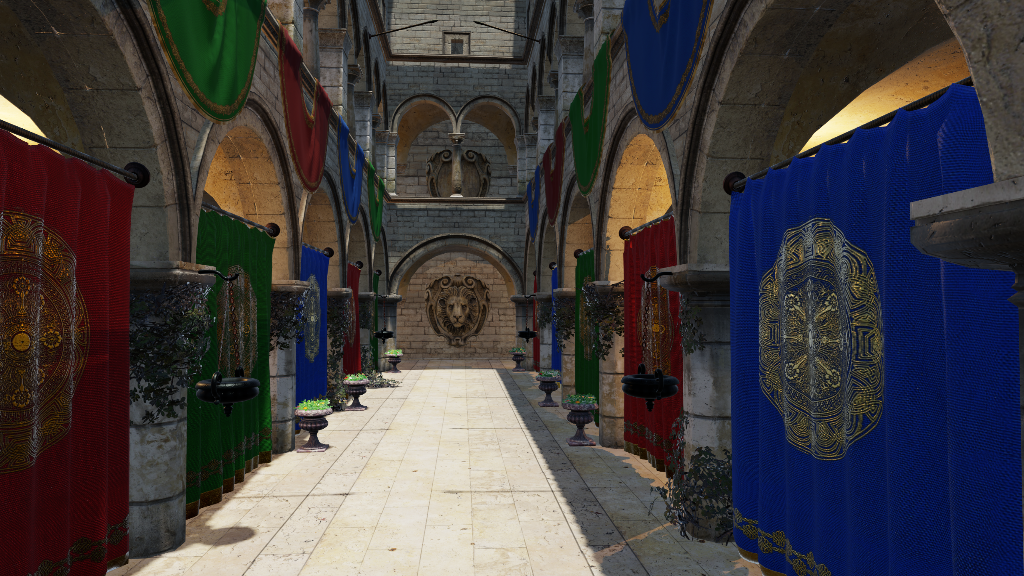
\includegraphics[width=0.82\textwidth]{figures/gi_off.png}

\vspace{6pt}

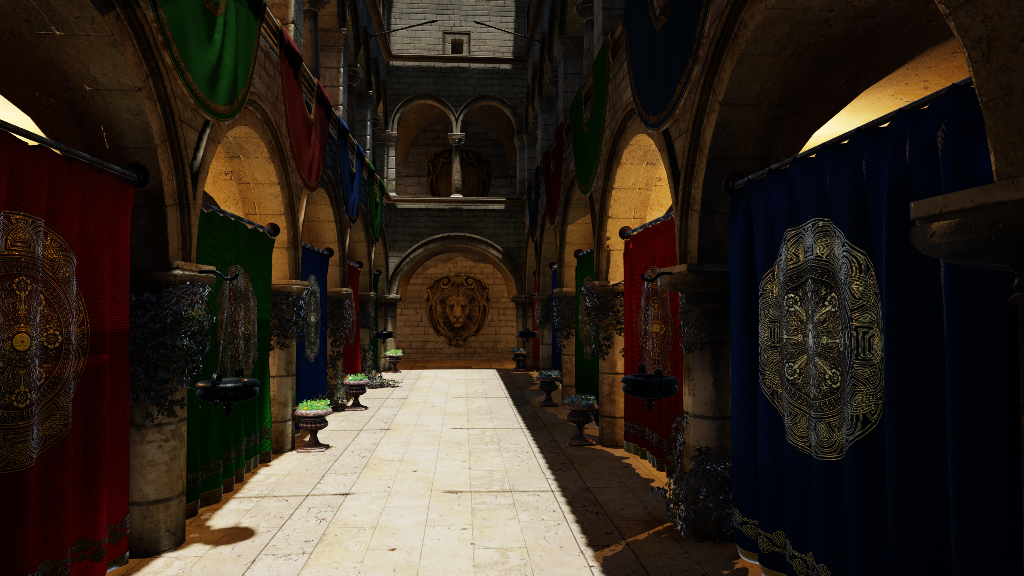
\includegraphics[width=0.82\textwidth]{figures/gi_on.png}
\caption[Scena bez globalnog osvetljenja i sa njim]{Scena bez (gore) i sa (dole) globalnim osvetljenjem: jedan difuzni indirektni odskok daje prelivanje boja i punjenje u senkama.}
\label{fig:gi-onoff}
\end{figure}

\section{Denoising (SVGF)}
\label{sec:denoising}

Svaki efekat ovde procenjuje integral po dolaznim pravcima iz jednog ili dva uzorka, a konvergencija $\sqrt{n}$ zna\v{c}i da sami uzorci ne mogu kupiti \v{c}istu sliku u okviru bud\v{z}eta frejma. Uzorci koji nedostaju postoje, samo ne u ovom pikselu i ovom frejmu: susedni pikseli obi\v{c}no gledaju skoro istu povr\v{s}inu, a prethodni frejm obi\v{c}no sadr\v{z}i istu povr\v{s}inu pomerenu za mali pomak kamere. Denoiser te uzorke pozajmljuje prostorno i temporalno, odbijaju\'ci da pozajmi preko prave ivice, gde je sused druga povr\v{s}ina i usrednjavanje bi razmazalo sliku. Odlu\v{c}ivanje \v{s}ta se ra\v{c}una kao ``ista povr\v{s}ina'' je cela pote\v{s}ko\'ca i razlog za\v{s}to denoiseru trebaju dubina i normale iz G-bafera, a ne samo boja. Slika~\ref{fig:gi-denoise-ab} u Glavi~\ref{ch:analiza} pokazuje \v{s}ta se time dobija: sirov GI bafer u polovini rezolucije naspram istog bafera posle temporalne akumulacije i \`a-trous filtera.

Snowstorm implementira varijantu Spatiotemporal Variance-Guided Filtering-a (SVGF) \cite{schied2017svgf}, standardnog filtera za rekonstrukciju efekata path tracing-a u realnom vremenu, kao jednu komponentu nezavisnu od signala. Jedna klasa \texttt{Denoiser} (\texttt{Render/Denoiser.\{hpp,cpp\}}) pokre\'ce temporalnu akumulaciju i prostorni \`a-trous filter, sa svim GPU stanjem po viewport-u (istorija, momenti, ping-pong scratch teksture) u komponenti \texttt{DenoiserInstance} koju poziv poseduje. Instancira se \v{c}etiri puta, za senke, GI, AO i refleksije, svaki sa sopstvenom konfiguracijom, ali istim kodom (Slika~\ref{fig:svgf}). Ponovna upotreba je mogu\'ca jer su za\v{s}umljena procena, njeni ulazi varijanse i G-bafer dubine/normala jedini podaci specifi\v{c}ni za signal. Te\v{z}ina zaustavljanja ivica po rastojanju pogotka povezana je za svaki signal, ali je podrazumevano ostavljena na nuli, pa je taj \v{c}lan bez efekta u izmerenoj konfiguraciji. Stohasti\v{c}ka putanja senki umesto toga veli\v{c}inu jezgra odre\dj{}uje direktno prema rastojanju okludera, u NRD SIGMA stilu, preko \texttt{render.shadows.denoise.penumbra}. Refleksije ponovo koriste GI-jev temporalni \v{s}ejder, \v{s}to je ograni\v{c}enje, jer istorija refleksije ima sadr\v{z}aj zavisan od pogleda koji reprojekcija pode\v{s}ena za difuzno ne obra\dj{}uje savr\v{s}eno.

\begin{figure}[tbp]
\centering
\begin{tikzpicture}[>={Stealth[]}, node distance=5mm,
  box/.style={draw, rounded corners, align=center, text width=10.6cm, inner sep=4pt, font=\small}]
  \node[box] (in)  {Za\v{s}umljen ulaz (GI, AO i stohasti\v{c}ke senke u polovini rezolucije, refleksije u punoj)};
  \node[box, below=of in]  (tp) {\textbf{Temporalno:} reprojekcija vektorima kretanja, akumulacija istorije
    (do 32 frejma), procena varijanse po pikselu};
  \node[box, below=of tp]  (at) {\textbf{\`A-trous prostorni filter:} 3 iteracije za GI i AO, 0 za
    refleksije (do 5), korak $1, 2, 4, \dots$; zaustavljanje ivica po normali, dubini i varijansi};
  \node[box, below=of at]  (out){Denoisovano, pa upsample-ovano (signali u polovini rezolucije), u prolaz
    Forward};
  \draw[->] (in) -- (tp); \draw[->] (tp) -- (at); \draw[->] (at) -- (out);
\end{tikzpicture}
\caption[Zajedni\v{c}ki SVGF denoiser]{SVGF denoiser: temporalna akumulacija sa procenom varijanse, pa prostorni \`a-trous filter vo\dj{}en varijansom. Jedna implementacija slu\v{z}i GI, AO, refleksijama i stohasti\v{c}koj putanji senki. GI i AO podrazumevano rade tri \`a-trous iteracije, a refleksije nijednu, iz razloga izmerenog u Odeljku~\ref{sec:denoise-eval}. Podrazumevana inline putanja senki uop\v{s}te ne ulazi u ovaj lanac.}
\label{fig:svgf}
\end{figure}

\subsection{Temporalna akumulacija}

Temporalni prolaz (\texttt{GITemporal.comp.hlsl}, u rezoluciji pra\'cenja) reprojektuje rezultat prethodnog frejma vektorima kretanja (\texttt{prev_uv = uv - velocity}) i me\v{s}a ga sa trenutnim za\v{s}umljenim ulazom. Uzorci van ekrana i prvi frejm resetuju se na trenutni ulaz, a test relativne dubine odbacuje disokludirane piksele. Me\v{s}anje sledi SVGF \v{s}emu du\v{z}ine istorije: akumulirana du\v{z}ina istorije po pikselu, ograni\v{c}ena na 32 frejma, postavlja te\v{z}inu me\v{s}anja \texttt{max(alphaMin, 1 / historyLength)}, pa tek disokludiran piksel sna\v{z}no te\v{z}i trenutnom frejmu, dok dugove\v{c}an piksel usrednjava mnogo frejmova. Prvi i drugi moment luminanse akumuliraju se istom te\v{z}inom, a njihova razlika je temporalna varijansa koja vodi prostorni filter. Pikseli premladi za stabilnu temporalnu varijansu (istorija kra\'ca od \v{c}etiri frejma) vra\'caju se na procenu prostorne varijanse u prozoru $7\times7$.

Preko osnovnog SVGF-a dodat je clamp boje u susedstvu: reprojektovana istorija se odseca ka srednjoj vrednosti susedstva $3\times3$ trenutnog frejma, ubla\v{z}en kad je piksel stati\v{c}an, a poo\v{s}tren kad se kre\'ce. Ovaj clamp u TAA stilu potiskuje duhove na pokretnim ivicama i u refleksijama, gde samo odbacivanje po dubini/normali nije dovoljno.

\subsection{Prostorni \`a-trous filter}

Prostorni prolaz (\texttt{GIDenoise.comp.hlsl}) je \`a-trous wavelet filter u jezgru SVGF-a: svaka iteracija je gather sa $5\times5$ odbiraka B3-spline jezgrom, a uzastopne iteracije udvostru\v{c}uju korak (\texttt{step = 1 << i}). Engine izvr\v{s}ava do pet iteracija, podesivo po signalu. Pri podrazumevanih tri (Slika~\ref{fig:atrous}) kumulativni domet je $2(1+2+4) = 14$ teksela, oslonac $29\times29$ prikupljen sa $75$ odbiraka umesto $841$ koliko bi ko\v{s}tao gust gather. Rupe pla\'caju domet, a te\v{z}ine zaustavljanja ivica spre\v{c}avaju da \v{s}ire iteracije cure preko geometrije.

\begin{figure}[tbp]
\centering
\begin{tikzpicture}[font=\scriptsize, scale=0.2]
  \foreach \it/\stride/\xoff in {0/1/0, 1/2/22, 2/4/44} {
    \begin{scope}[xshift=\xoff cm]
      \draw[black!15] (-8.5,-8.5) grid (8.5,8.5);
      \foreach \dy in {-2,-1,0,1,2} \foreach \dx in {-2,-1,0,1,2} {
        \pgfmathsetmacro{\px}{\dx*\stride}
        \pgfmathsetmacro{\py}{\dy*\stride}
        \fill[black!62] (\px-0.5,\py-0.5) rectangle (\px+0.5,\py+0.5);
      }
      \fill[white] (-0.5,-0.5) rectangle (0.5,0.5);
      \draw[black, thick] (-0.5,-0.5) rectangle (0.5,0.5);
      \node[font=\small] at (0,-10.4) {iteracija \it, korak \stride};
      \node[font=\small] at (0,-12.6) {domet $\pgfmathparse{int(4*\stride+1)}\pgfmathresult
        \times \pgfmathparse{int(4*\stride+1)}\pgfmathresult$};
    \end{scope}
  }
\end{tikzpicture}
\caption[\`A-trous: rastu\'ci korak i domet filtera]{Tri iteracije a-trous filtera, sve nad istim ise\v{c}kom $17\times17$ oko filtriranog piksela (beli kvadrat u sredini). Svaka iteracija uzima istih 25 odbiraka, samo sa duplo ve\'cim korakom, pa domet raste dok cena po iteraciji ostaje ista. Rupe izme\dj{}u odbiraka pla\'caju domet: kumulativno $29\times29$ sa 75 odbiraka umesto 841.}
\label{fig:atrous}
\end{figure}

Svaki odbirak nosi tri \v{c}lana zaustavljanja ivica (Listing~\ref{lst:atrous}): normalu, relativnu linearizovanu dubinu i \v{c}lan luminanse vo\dj{}en varijansom, koji je defini\v{s}u\'ca ideja SVGF-a. Po\v{s}to te\v{z}ina luminanse raste sa kvadratnim korenom filtrirane varijanse, filter agresivno zamu\'cuje gde je signal \v{s}umovit, a \v{c}uva detalj gde je konvergirao. Sama varijansa se filtrira kvadratima te\v{z}ina odbiraka, a svi vode\'ci baferi se uzorkuju bez interpolacije (point-sampled) da bi se izbeglo curenje preko ivica. Isklju\v{c}ivanje \v{c}lana varijanse (\texttt{LumaPhi = 0}) svodi filter na obi\v{c}an bilateralni blur, korisnu osnovnu liniju u Glavi~\ref{ch:analiza}.


\needspace{12\baselineskip}
\begin{lstlisting}[caption={Te\v{z}ine zaustavljanja ivica za \`a-trous filter (SVGF jezgro, HLSL).}, label={lst:atrous}]
float w_n = pow(saturate(dot(N, N_tap)), K_NORMAL);              // normal
float w_z = exp(-abs(z - z_tap) / (K_DEPTH * abs(dzdx) + 1e-4)); // depth
float w_l = exp(-abs(lum - lum_tap) /                            // variance-guided luminance
                (LUMA_PHI * sqrt(varBlur) + 1e-4));
float w   = w_n * w_z * w_l * kernel[dy + 2] * kernel[dx + 2];   // combined tap weight
sum  += w * color_tap;
wSum += w;
\end{lstlisting}

\subsection{Odstupanja od SVGF-a i njihova cena}

Implementacija odstupa od rada na \v{c}etiri mesta, sva navedena da bi se brojevi kvaliteta iz Glave~\ref{ch:analiza} \v{c}itali ispravno:
\begin{itemize}
\item denoiser filtrira sirovu iradijansu i ponovo mno\v{z}i albedo posle upsample-a, dok SVGF demoduli\v{s}e unutar filtera,
\item dodatni temporalni clamp boje gore nije u SVGF-u,
\item GI i AO se filtriraju u polovini rezolucije, dok je SVGF u punoj rezoluciji,
\item zaustavljanje ivica po varijansi je opciono.
\end{itemize}

Izbor na nivou izvornog koda koji ne mo\v{z}e promeniti izlaznu sliku, na primer da li je jedna petlja odmotana, odlu\v{c}uje da li \v{s}ejder dobija 16 od 16 wavefront-ova ili 8. \texttt{GIDenoise.comp} dr\v{z}i svoju spoljnu \`a-trous petlju neodmotanom, \v{s}to ko\v{s}ta malo slobode raspore\dj{}ivanja, a zauzvrat dr\v{z}i pritisak na registre na 58 VGPR-ova na RX 9070 XT, bez spilovanja i sa punom zauzeto\v{s}\'cu (Tabela~\ref{tab:occupancy}). Odmotana alocira 191, prelaze\'ci granicu alokacije koju 58 ne prelazi, i pada na 8 od 16 wavefront-ova.

\section{TAA / temporalni resolve}
\label{sec:taa}

Po\v{s}to forward prolaz proizvede osen\v{c}enu HDR sliku, temporalni anti-aliasing resolve \cite{karis2014taa} (\texttt{TemporalResolvePass}, \texttt{TemporalResolve.frag.hlsl}) akumulira je kroz frejmove da ukloni aliasing i da konvergira preostali \v{s}um koji denoiseri po efektu ostavljaju. Kamera se u svakom frejmu pomera za pod-piksel na niskodiskrepantnoj sekvenci od 16 faza, pa uzastopni frejmovi uzorkuju razli\v{c}ite ta\v{c}ke unutar piksela, a resolve reprojektuje prethodni izlaz vektorima kretanja i odseca ga prema lokalnom susedstvu trenutnog piksela, labavo za stati\v{c}an piksel i stro\v{z}e pri kretanju (d\v{z}iter je Halton(2,3), reprojekcija koristi dilataciju najbli\v{z}e dubine da tanke strukture uzmu pravu brzinu i Catmull-Rom rekonstrukciju istorije radi smanjenja zamu\'cenja reprojekcije, a odsecanje je Karis zaobljena kutija nad susedstvom $3\times3$ u YCoCg prostoru).

Resolve radi u linearnom HDR-u i samo akumulira. To je namerna invarijanta: svaka perceptivna operacija ili operacija u prostoru prikaza (izo\v{s}travanje, kontrast) dr\v{z}i se van ovog prolaza i primenjuje posle tonemap-a, jer kriva po kanalu primenjena pre tonemap-a pretvara preba\v{c}aj akumulacije u pomak nijanse. Izo\v{s}travanje zato \v{z}ivi u zasebnom prolazu posle tonemap-a, a ne ovde, i taj prolaz je podrazumevano isklju\v{c}en (\texttt{render.sharpen} 0), pa ga ni\v{s}ta izmereno u Glavi~\ref{ch:analiza} ne pokre\'ce.

Vektori kretanja su zajedni\v{c}ki preduslov tri potro\v{s}a\v{c}a: SVGF temporalnog prolaza, TAA resolve-a i screen-space efekata koji uzorkuju boju pro\v{s}log frejma. Prolaz brzine (Slika~\ref{fig:motion}) renderuje scenu drugi put i pi\v{s}e po pikselu pomak ta\v{c}ke povr\v{s}ine u prostoru ekrana izme\dj{}u prethodne i trenutne view-projection matrice.

Re\v{z}im otkaza koji ovo izla\v{z}e je disokluzija. Piksel otkriven iza okludera u ovom frejmu nema prethodnu poziciju na koju bi pokazao, pa mu je istorija bez smisla, a njeno ponovno kori\v{s}\'cenje razmazalo bi boju okludera preko novootkrivene povr\v{s}ine. Svaka temporalna faza u engine-u zato uparuje reprojekciju sa testom odbacivanja po dubini i normali, a gde se on okine, piksel se vra\'ca samo na trenutni frejm, koji je \v{s}umovitiji, ali ispravan.

\begin{figure}[tbp]
\centering
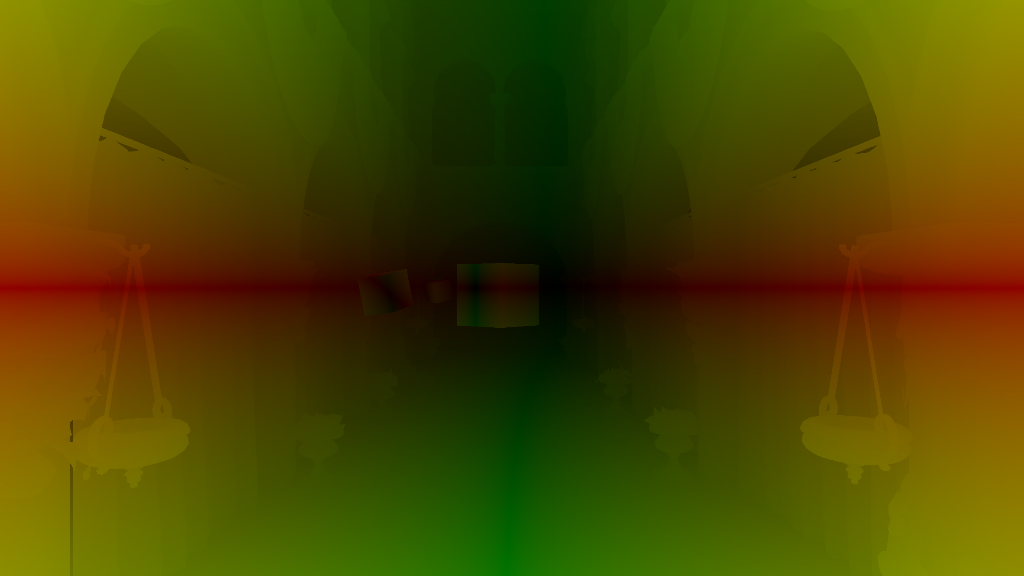
\includegraphics[width=0.8\textwidth]{figures/dbg_motion.png}
\caption[Debug prikaz vektora kretanja]{Bafer vektora kretanja (\texttt{render.debugview} 1) na \texttt{dolly} probi rute, na sceni sa animiranim rekvizitima. Crveno je horizontalni, a zeleno vertikalni pomak izme\dj{}u uzastopnih frejmova, u apsolutnoj vrednosti i skalirano sa 40, pa prikaz pokazuje intenzitet i osu, ali ne i smer. Kretanje napred daje radijalni uzorak: tamni centar je \v{z}ari\v{s}te \v{s}irenja, gde se povr\v{s}ine ka kojima se kamera kre\'ce jedva pomeraju. Pravougaone mrlje su rotiraju\'ci rekviziti, \v{c}iji se vektori prekidaju od zida iza njih, a taj prekid je gorenavedena disokluzija. Poni\v{s}tavanjem normalizacije po osi i sRGB kodiranja, srednji pomak je $0.24\%$ dijagonale ekrana, a najvi\v{s}e $0.75\%$, bez zasi\'cenog uzorka.}
\label{fig:motion}
\end{figure}

\section{Reproduktivnost i alati}
\label{sec:alati}

Merenja u Glavi~\ref{ch:analiza} poti\v{c}u iz instrumentacije ugra\dj{}ene u engine, zbog \v{c}ega su reproduktivna, a ne jednokratni snimci. Svaki efekat se uklju\v{c}uje i pode\v{s}ava kroz registar console promenljivih, pa je benchmark konfiguracija skup vrednosti CVar-ova, a ne izmena koda, podesiva iz komandne linije za headless pokretanja, a svaki prolaz grafa renderovanja obavijen je GPU timestamp opsegom. \v{C}etiri alata izgra\dj{}ena povrh toga (Tabela~\ref{tab:tooling}) porede se sa committovanom osnovnom linijom i obaraju pokretanje pri regresiji, \v{s}to i razdvaja kapiju od izve\v{s}taja: broj koji niko ne proverava lagano odlazi.

\begin{table}[tbp]
\caption[Alati za merenje]{Alati koji proizvode brojeve u Glavi~\ref{ch:analiza}. ``Kapija'' zna\v{c}i da alat poredi sa committovanom osnovnom linijom i obara pokretanje pri regresiji, dok alati bez kapije samo izve\v{s}tavaju. Svima osim \texttt{rga-occupancy} treba pravi GPU, pa rade lokalno, a ne na CI-ju.}
\label{tab:tooling}
\centering
\begin{tabular}{lp{0.55\textwidth}l}
\toprule
Alat & \v{S}ta meri & Kapija \\
\midrule
\texttt{perf-bench}     & GPU ms po prolazu, matrica konfiguracija; opciono pinovanje takta, uparena A/B presuda & da \\
\texttt{quality-bench}  & FLIP/PSNR/SSIM (LPIPS kad je dostupan) naspram path trace-a, stati\v{c}na kamera, fiksan \texttt{render.resolution} & da \\
\texttt{quality-motion} & FLIP, tFLIP, lag i JOD du\v{z} rute & da \\
\texttt{rga-occupancy}  & pritisak na registre i zauzetost, offline & da \\
\texttt{quality-tune}   & pretraga CVar-ova naspram reference & ne \\
\texttt{smoke-test}     & pad, zamrzavanje, Vulkan validacija & prolazi/pada \\
\texttt{shader-stats}   & registri koje prijavljuje drajver, oba vendora & ne \\
Tracy + watchdog        & vremenska linija po sistemu, zastoji po frejmu & ne \\
\bottomrule
\end{tabular}
\end{table}

\section{Referentni path tracer}
\label{sec:pathtracer}

Referenca je brute-force jednosmerni path tracer ugra\dj{}en u engine (\texttt{PathTrace\allowbreak.comp\allowbreak.hlsl}): next-event estimation ka suncu, isti metallic-roughness mikrofasetni BSDF kao forward \v{s}ejdiranje, vi\v{s}eodsko\v{c}no indirektno osvetljenje sa prekidom ruskom ruletom i progresivna akumulacija u trajni HDR bafer dok je kamera stati\v{c}na. Sunce se uzorkuje kao kona\v{c}an disk kroz istu \texttt{SampleCone} rutinu i isti poluugao \texttt{render.shadow.sun\_angle\_deg} kao putanja mekih senki u realnom vremenu, pa se svaka razlika u penumbri mo\v{z}e pripisati uzorkovanju i rekonstrukciji, a ne druga\v{c}ijem modelu svetla (nebo pri proma\v{s}aju zraka dodaje se bez diska sunca, da se izbegne dvostruko ra\v{c}unanje). Po\v{s}to senke, ambijentalna okluzija, refleksije i indirektno svetlo proizlaze iz istog vi\v{s}eodsko\v{c}nog transporta, jedan konvergirani path trace je ground truth za sve njih odjednom (Slika~\ref{fig:pt-ref}). Akumulira 2 putanje po pikselu po frejmu tokom najmanje 400 frejmova, dakle najmanje 800 putanja po pikselu, pri maksimalnoj du\v{z}ini putanje 8 sa prekidom ruskom ruletom, a snimak se dr\v{z}i dok ne pro\dj{}e test konvergencije, umesto da se zaustavi na fiksnom broju. Kapija ga pokre\'ce \emph{nepristrasno}, sa isklju\v{c}enim i clamp-om fireflies-a i clamp-om te\v{z}ine regularizacije putanje, jer bi clamp-ovana referenca pristrasila upravo energiju prema kojoj se tehnike u realnom vremenu ocenjuju. Postoji samo kao oslonac ispravnosti. Obe strane svakog pore\dj{}enja prolaze kroz isti tonemap lanac, pa je uklju\v{c}ivanje path tracer-a A/B pore\dj{}enje jabuka sa jabukama, a ne pore\dj{}enje HDR i LDR slike.

\begin{figure}[tbp]
\centering
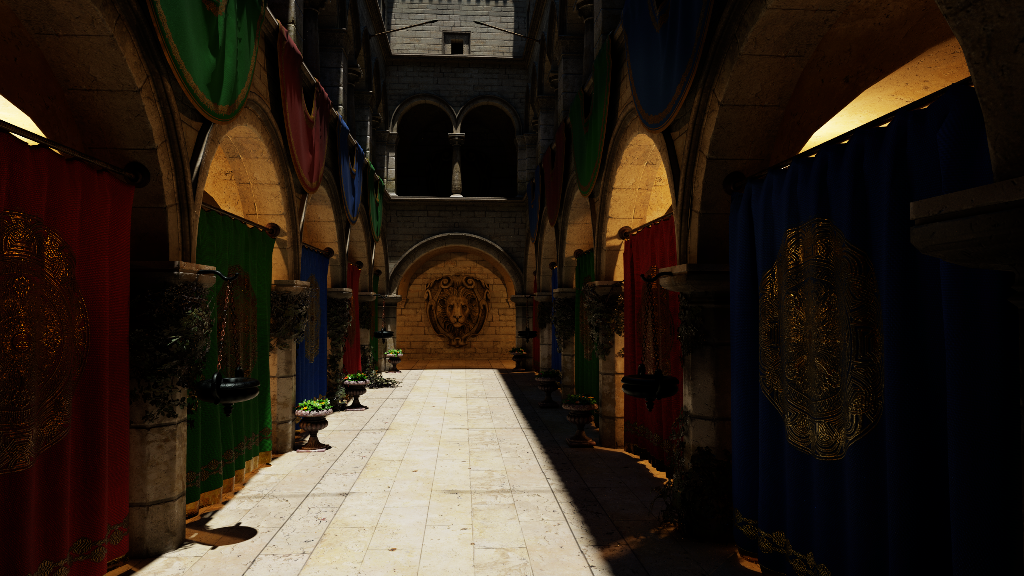
\includegraphics[width=0.85\textwidth]{figures/pt_ref.png}
\caption[Konvergirani referentni frejm path tracer-a]{Konvergirani referentni frejm ugra\dj{}enog path tracer-a, prema kome se svaka tehnika u realnom vremenu meri preko FLIP/PSNR/SSIM.}
\label{fig:pt-ref}
\end{figure}

\section{Uslovi i pretpostavke}
\label{sec:uslovi}

Implementacija pravi nekoliko namernih aproksimacija da ostane u bud\v{z}etu realnog vremena, svaka je pojednostavljenje punog problema, a ne faktor koji iskrivljuje relativna merenja u Glavi~\ref{ch:analiza}.

\begin{itemize}
  \item \textbf{Difuzno GI sa jednim odskokom.} Globalno osvetljenje ra\v{c}una jedan difuzni indirektni odskok, dok su vi\v{s}eodsko\v{c}no i sjajno indirektno osvetljenje van opsega.
  \item \textbf{GI i AO u polovini rezolucije.} GI i AO se prate u polovini rezolucije i bilateralno upsample-uju. Refleksije se prate u punoj rezoluciji.
  \item \textbf{Mali broj uzoraka uz rekonstrukciju.} Efekti koriste jedan ili dva zraka po pikselu i za upotrebljivu sliku zavise od temporalne akumulacije, a za GI i AO i od prostornog SVGF filtera. Prostorni filter je za refleksije isklju\v{c}en (Odeljak~\ref{sec:denoise-eval}).
  \item \textbf{Pribli\v{z}ne meke senke.} U podrazumevanoj putanji senke pra\'cenjem zraka koriste jedan tvrd ili dva meka zraka po svetlu, prate se inline i primenjuju direktno bez denoisera, pa je penumbra dvouzorkovna aproksimacija povr\v{s}inskog svetla koju \v{c}isti samo temporalni resolve, a ne konvergirana meka senka. Opciona stohasti\v{c}ka putanja rekonstrui\v{s}e svoju agregatnu vidljivost kroz zajedni\v{c}ki denoiser, po ceni razre\v{s}avanja samo jednog svetla po pikselu po frejmu.
  \item \textbf{Samo inline ray query-ji.} Nema ray tracing pipeline-a, shader binding table-a ni rekurzije. Svo osvetljenje pogotka je jedan odskok evaluiran u \texttt{ShadeSurfaceHit}.
  \item \textbf{NEE lokalnih svetala sa jednim uzorkom, samo GI.} Sekundarni pogodak GI dodaje najvi\v{s}e jedno od ta\v{c}kastih i spot svetala scene, izabrano importance sampling-om po pogotku, a ne sumirano preko svih, pa ostaje \v{s}umovit estimator sa jednim uzorkom pune next-event estimation, a ne ta\v{c}na suma. Pogoci refleksija uop\v{s}te nisu pro\v{s}ireni lokalnim svetlima (\texttt{render.rt.hit_lights} nije izmerio dobitak kvaliteta tu za dvostruku cenu na GI strani).
  \item \textbf{Potpuna ponovna izgradnja TLAS-a po dinami\v{c}nom frejmu.} Struktura najvi\v{s}eg nivoa ponovo se gradi, a ne osve\v{z}ava, u svakom frejmu u kom se scena menja, iako potpuno stati\v{c}na scena preska\v{c}e ponovnu izgradnju.
\end{itemize}

\chapter{Analiza}
\label{ch:analiza}

Svaki broj u ovoj glavi dolazi iz izmerenog pokretanja. Glava je duga, pa su njeni nalazi prvo sakupljeni ovde, svaki sa odeljkom koji ga utvr\dj{}uje.

\begin{itemize}
\item Sva \v{c}etiri efekta zajedno ko\v{s}taju \perfFourEffectsAMD{} ms na RX 9070 XT i
      \perfFourEffectsNV{} ms na RTX 5070, \v{s}to je na obe kartice unutar frejma od 60 Hz
      (Odeljak~\ref{sec:cena}).
\item Dve kartice se ne sla\v{z}u oko toga koji je efekat skup, a neslaganje dopire do in\v{z}enjerske odluke: od dve strategije za senke svaka je jeftinija na jednoj kartici
      (Odeljci~\ref{sec:cena} i \ref{sec:analiza-shadow-strategy}).
\item Vi\v{s}e zraka donosi veoma malo. Osam puta ve\'ci bud\v{z}et vra\'ca \rcPsnrGain{} dB PSNR-a za
      \rcGpuPct\% vi\v{s}e GPU vremena, pa je radna ta\v{c}ka jedan zrak po pikselu
      (Odeljak~\ref{sec:raycount}). Pra\'cenje u polovini rezolucije pona\v{s}a se isto
      (Odeljak~\ref{sec:halfres}).
\item Prostorni denoiser opravdava svoju cenu stabilno\v{s}\'cu, a ne ta\v{c}no\v{s}\'cu na mirnoj slici: stati\v{c}ke metrike pomera za manje od \v{s}uma merenja, a treperenje izme\dj{}u frejmova
      smanjuje za \flickerPct\% (Odeljci~\ref{sec:denoise-eval} i \ref{sec:motion}).
\item Pra\'cenje zraka najvi\v{s}e podi\v{z}e kvalitet tamo gde rasterizacija ima najmanje \v{s}ta da
      radi, pa FLIP pada sa \qRasterFlip{} na \qAllRtFlip{}, uz globalno osvetljenje kao dominantan \v{c}lan
      (Odeljak~\ref{sec:poredjenje}).
\item Ugradnja ray query-ja u liniji ko\v{s}ta zauzetost: forward \v{s}ejder prelazi sa 87 na 130 registara, a sa
      16 istovremeno rezidentnih talasa na 10 (Odeljak~\ref{sec:occupancy}).
\end{itemize}

Dve stvari se ponavljaju i ovde se navode jednom, umesto u svakom odeljku. Cene se \v{c}itaju sa \emph{lestvice} konfiguracija, gde svaka \emph{prečka} dodaje jedan efekat, pa je cena efekta
razlika izme\dj{}u susednih pre\v{c}ki. I svaka razlika se \v{c}ita naspram praga ponovljivosti
utvr\dj{}enog u Odeljku~\ref{sec:metodologija}, ispod kog ovaj protokol ne mo\v{z}e da razdvoji dve
konfiguracije, zbog \v{c}ega je nekoliko rezultata ispod prijavljeno kao nepostojanje razlike, a ne kao
mala razlika.

\section{Metodologija}
\label{sec:metodologija}

\paragraph{Hardver: me\dj{}uvendorska postavka.} Centralna evaluacija poredi identi\v{c}an pipeline na
dve grafi\v{c}ke kartice aktuelne generacije od razli\v{c}itih proizvo\dj a\v{c}a: AMD Radeon RX 9070 XT (RDNA4) i NVIDIA
GeForce RTX 5070 (Blackwell), navedene u Tabeli~\ref{tab:gpus}. Obe pokre\'cu isti binarni fajl engine-a,
iste SPIR-V \v{s}ejdere, isti graf renderovanja i istu scenu sa istim pode\v{s}avanjima. Jedina promenljiva je
izabrani fizi\v{c}ki ure\dj{}aj, \v{s}to je osnova poštenja: svaka razlika u vremenu poti\v{c}e od
hardvera i drajvera, a ne od druge putanje koda, dok bi razilaženje kvaliteta ukazivalo na
nedeterminizam vredan istrage, a ne na stvarnu razliku. Jedini dokumentovani izuzetak od tvrdnje o identi\v{c}noj putanji koda je podr\v{s}ka za opacity micromap.

\begin{table}[tbp]
\caption[Grafi\v{c}ke kartice u me\dj{}uvendorskom poređenju]{Grafi\v{c}ke kartice u me\dj{}uvendorskom poređenju, prema slu\v{z}benim specifikacijama proizvo\dj a\v{c}a
(AMD, NVIDIA) i verzijama drajvera na ma\v{s}ini za testiranje.}
\label{tab:gpus}
\centering
\begin{tabularx}{\textwidth}{l >{\raggedright\arraybackslash}X >{\raggedright\arraybackslash}X}
\toprule
 & AMD RX 9070 XT & NVIDIA RTX 5070 \\
\midrule
Arhitektura            & RDNA4 (Navi 48) & Blackwell (GB205) \\
Compute jedinice / SM  & 64 CU, 4096 stream procesora & 48 SM, 6144 CUDA jezgra \\
RT akceleratori        & 64 (3. generacija) & 48 \\
Takt (boost)           & 2970 MHz & 2512 MHz \\
Memorija / propusnost  & 16 GB GDDR6, 640 GB/s & 12 GB GDDR7, 672 GB/s \\
TDP (TBP / TGP)        & 304 W & 250 W \\
Drajver / OS           & 32.0.31035.1003, Windows 11 Pro (build 26100) & 32.0.15.9186, Windows 11 Pro (build 26100) \\
\bottomrule
\end{tabularx}
\end{table}

Dva reda koja najvi\v{s}e li\v{c}e na rang-listu su ona koja se najmanje mogu porediti. Stream procesor
i CUDA jezgro nisu ista jedinica posla, pa 4096 prema 6144 nije faktor 1.5 ni u \v{c}emu, a broj RT
akceleratora ima razli\v{c}it smisao kod svakog proizvo\dj a\v{c}a upravo zato \v{s}to dva proizvo\dj a\v{c}a razli\v{c}ito dele
obilazak (Odeljak~\ref{sec:accel-pregled}). Kartice su uparene po onome \v{s}to se mo\v{z}e porediti:
propusnost memorije u okviru 5\%, ista generacija procesa i susedni polo\v{z}aji u linijama proizvoda. Gde se u merenjima koja slede razilaze,
strukturni kandidat je ta podela obilaska, a ne bilo koji pojedinačni broj iz ove tabele, a
Odeljak~\ref{sec:cena} pokazuje da odnos po prolazu obuhvata raspon od \perfRatioMin{} do \perfRatioMax{}, koji nijedna
pojedina\v{c}na hardverska vrednost ne mo\v{z}e da proizvede.

\paragraph{Nepodudaranje podr\v{s}ke za OMM.} Sponza ima tri MASK materijala (alfa-isecanje), koji se prate
kroz opacity-micromap BLAS na ure\dj{}aju koji izla\v{z}e \texttt{VK\_EXT\_opacity\_micromap}, a inače
kroz rezervni any-hit alfa-test (Odeljak~\ref{sec:accel}). Drajver RTX 5070 izla\v{z}e ekstenziju, a drajver 9070 XT ne, uprkos uporedivim hardverskim mogu\'cnostima, pa
dva proizvo\dj a\v{c}a ovde razre\v{s}avaju maskiranu geometriju kroz zaista razli\v{c}it kod strukture ubrzanja. Ta
razlika menja samo na\v{c}in na koji se maskirani mikrotrougao klasifikuje tokom obilaska, a ne pravac zraka,
poziciju pogotka ni \v{s}ejding, pa je lo\v{s} kandidat za razliku u metrici kvaliteta: pe\v{c}enje je
konzervativno i svaki mikrotrougao \v{c}iji se barycentric uzorci ne sla\v{z}u \v{s}alje u stanje
\texttt{UNKNOWN} koje i dalje izvr\v{s}ava ta\v{c}an any-hit alfa-test, pa do rezolucije te mre\v{z}e uzoraka
ekstenzija menja koliko obilazak ko\v{s}ta, a ne \v{s}ta nalazi. To je mali jednosmerni doprinos koji zavisi od drajvera, u razlici u GPU-ms po efektu gde god zrak pogodi isečenu
geometriju, i ova evaluacija ga dalje ne izoluje.

\paragraph{Scena i kontrole.} Test scena je Sponza, standardni enterijer sa jakim indirektnim
odbijanjem, osvetljen sa pet uklju\v{c}enih svetala: \v{c}etiri ta\v{c}kasta (baklje) i jedno usmereno (sunce). Tri reflektorska svetla i
dva dodatna ta\v{c}kasta su definisana ali isklju\v{c}ena, a razlika je bitna jer podrazumevana
putanja senki ko\v{s}ta dva zraka po svetlu po pikselu.

Jedno svojstvo rasterske putanje ograni\v{c}ava svaku tehniku koja je koristi: engine alocira najvi\v{s}e dve
omni mape senki (\texttt{MAX\_SHADOW\_POINTS}, \v{s}est prolaza dubine svaka), pa dva od \v{c}etiri uklju\v{c}ena
ta\v{c}kasta svetla renderuju bez senke. Senke sa pra\'cenjem zraka nemaju takvo ograni\v{c}enje i prate svako svetlo, pa
svaka tehnika u Tabeli~\ref{tab:quality} osim \texttt{all-RT} stoji na slabijoj osnovi senki
nego renderer bez tog ograni\v{c}enja, \v{s}to ide u korist strane sa pra\'cenjem zraka. Efekat je ograni\v{c}en i
mali: sama tehnika senki pomera PSNR za 0.65 dB od \qRtLiftPsnr{} dB izme\dj{}u rastera i svih efekata,
a FLIP za 0.024 od 0.349, pa u pobolj\v{s}anju iz Odeljka~\ref{sec:poredjenje} dominira globalno
osvetljenje, a ne ovo ograni\v{c}enje.

Dve porodice merenja u ovoj glavi ne dele rezoluciju, jer se izvode na razli\v{c}itim mestima. Vremena dolaze iz editora u
$\perfWidth{} \times \perfHeight{}$, veli\v{c}ini koju svaka osnovna linija bele\v{z}i kako bi se pokretanje u drugoj
preskakalo umesto upore\dj ivalo, dok snimci kvaliteta koriste runtime bez editora i
pre ocenjivanja se resampluju na kanonsku veli\v{c}inu. Zato se cene porede sa cenama, a ocene sa ocenama, nikad
me\dj{}usobno. Za svako A/B kamera je statična,
jer pokretna kamera desinhronizuje niz frejmova izme\dj{}u dva pokretanja i izmi\v{s}lja razlike koje su
artefakti vremena. Ke\v{s} \v{s}ejdera se bri\v{s}e pre nego \v{s}to se poveruje bilo kojoj GPU metrici, jer
zastareo ke\v{s} daje nedeterministi\v{c}ke rezultate, a sa\v{c}uvane konzolne promenljive se tokom benchmark pokretanja ignori\v{s}u, pa preostalo pode\v{s}avanje ne mo\v{z}e neprimetno da promeni konfiguraciju.

\paragraph{Merenje performansi.} GPU vreme dolazi iz timestamp opsega po prolazu i
\texttt{perf-bench} alata iz Odeljka~\ref{sec:alati}, usrednjeno preko fiksnog bud\v{z}eta frejmova kad se
stabilno stanje detektuje, a ne pretpostavi: vreme frejma se na ovoj sceni sti\v{s}ava tek posle oko pedeset frejmova, pa bi
fiksno kratko zagrevanje u rezultat usrednjilo deo rasta takta, u iznosu koji zavisi od toga koliko je ma\v{s}ina ve\'c bila topla, bez ikakvog traga u izlazu.
Benchmark prolazi fiksnu matricu konfiguracija, uklju\v{c}uju\'ci po jedan efekat vi\v{s}e u svakom koraku, pa je
cena efekta razlika izme\dj{}u susednih (Tabela~\ref{tab:cena}). Razlika, a ne izolovano merenje, jer
efekti dele fiksni posao: struktura ubrzanja se gradi jednom, G-bafer se puni jednom, tonemap se izvr\v{s}ava jednom, pa bi merenje jednog efekta samog njemu
naplatilo sve to i \v{c}etiri vrednosti bi u zbiru daleko prelazile frejm. Razlika se uzima na \emph{ukupnom}
GPU vremenu, a ne na opsegu jednog prolaza, jer se inline senke prate unutar Forward prolaza i
nemaju sopstveni, a ostala tri se prijavljuju isto radi doslednosti. Timestampovi se
pretvaraju periodom timestampa svakog ure\dj{}aja, pa su vremena po prolazu uporediva izme\dj{}u proizvo\dj a\v{c}a.

\paragraph{Merenje kvaliteta.} Kvalitet rekonstrukcije meri \texttt{quality-bench} naspram
konvergirane path-traced reference iz Odeljka~\ref{sec:pathtracer}. Tonemapirani prikaz svake tehnike u realnom vremenu
ocenjuje se naspram nje merom \textbf{FLIP} (perceptivna) \cite{andersson2020flip},
\textbf{PSNR} i \textbf{SSIM} \cite{wang2004ssim}. FLIP je primarna jer modeluje ono \v{s}to posmatra\v{c}
primećuje, a ne sirovu gre\v{s}ku po pikselu. PSNR strukturno favorizuje zamu\'cenu sliku, a SSIM poredi lokalnu strukturu, a ne
apsolutne vrednosti, pa se prijavljuju sve tri i nijedna pristrasnost jedne metrike ne odlu\v{c}uje o zaklju\v{c}ku.
Ocene se usrednjuju preko tri fiksne orijentacije iz jedne unutra\v{s}nje pozicije (niz glavni brod, nagnuto
ka podu, nagnuto ka gornjoj galeriji), izabrane tako da razli\v{c}ito optere\'cuju ambijentalnu okluziju, globalno osvetljenje
i refleksije, pa jedno kadriranje ne mo\v{z}e da pristrasno utiče na rezultat. Svaki snimak se prvo bilinearno
resamplira na kanonsku $1024 \times 576$, pa razlika u veli\v{c}ini prozora izme\dj{}u pokretanja ne mo\v{z}e neprimetno da promeni ocenu. Vrednosti kvaliteta na drugim mestima u ovoj glavi
su sa RX 9070 XT, iako Odeljak~\ref{sec:cross-vendor-quality} snima celu matricu i na
RTX 5070.

Ova glava koristi ukupno \v{s}est mera, tri za mirnu sliku i tri koje zahtevaju kretanje.
Tabela~\ref{tab:metrics} ih sakuplja, sa smerom u kom se pobolj\v{s}avaju i najmanjom
razlikom koju ovaj protokol mo\v{z}e da razre\v{s}i, da \v{c}italac koji na neku naiđe kasnije ne mora
da je rekonstrui\v{s}e iz teksta u kom je uvedena.

\begin{table}[tbp]
\caption[Mere kori\v{s}\'cene u ovoj glavi]{Mere kori\v{s}\'cene u ovoj glavi i najmanja
razlika koju svaka mo\v{z}e da razre\v{s}i. Tri praga su ponovljivost, izmerena ponovnim snimanjem cele
matrice i o\v{c}itavanjem koliko su se pet tehnika koje nisu mogle da se promene ipak pomerile
(petnaest snimaka), metodom iz pasusa ispod. Mere kretanja nemaju sopstveni prag
ovde, jer su snimljene jednom, a ne ponovo.}
\label{tab:metrics}
\centering
\small
\begin{tabularx}{\textwidth}{@{}l>{\raggedright\arraybackslash}X c r@{}}
\toprule
Mera & \v{S}ta poredi & Bolje & Prag \\
\midrule
FLIP  & frejm naspram path-traced reference, ponderisano onim \v{s}to posmatra\v{c} primeti\'ce & ni\v{z}e & 0.0024 \\
PSNR  & isto, kao logaritam srednje kvadratne gre\v{s}ke, \v{s}to favorizuje zamu\'cenu sliku & vi\v{s}e & 0.06 dB \\
SSIM  & isto, kao lokalna struktura, a ne apsolutne vrednosti piksela & vi\v{s}e & 0.0022 \\
\addlinespace[3pt]
tFLIP & koliko se tehnika menja izme\dj{}u susednih frejmova, preko onoga koliko se referenca menja u istom intervalu & ni\v{z}e & -- \\
kašnjenje & pokretni frejm naspram sopstvenog konvergiranog mirnog frejma ovog renderera u istoj pozi & ni\v{z}e & -- \\
JOD   & ColorVideoVDP, jedina mera ovde koja direktno modeluje temporalnu osetljivost na kontrast, gde je 1 JOD otprilike 75\% preferencije populacije & vi\v{s}e & -- \\
\bottomrule
\end{tabularx}
\end{table}

Nekoliko rezultata ispod zavisi od razlike koja je premala da bi se pro\v{c}itala, pa ti pragovi moraju
odnekud da dođu. Ponovno snimanje cele matrice posle promene denoisera daje ih bez posebnog
eksperimenta: pet tehnika (\texttt{raster}, \texttt{ssao}, \texttt{ssr}, \texttt{rtao},
\texttt{rtrefl}) ne izvr\v{s}ava filter koji se promenio, pa je ono za \v{s}ta su se njihove ocene pomerile
ponovljivost, a ne efekat. Tri koje ga izvr\v{s}avaju pomerile su se do 0.0096 FLIP, \v{c}etiri puta vi\v{s}e od
praga, \v{s}to je razdvajanje koje metodu \v{c}ini vrednom. To je jedno ponovno snimanje, a ne
studija ponovljenih merenja, pa vrednosti iz Tabele~\ref{tab:metrics} treba \v{c}itati kao pravi red
veli\v{c}ine, a ne kao intervale poverenja.

\section{Cena po efektu (GPU ms)}
\label{sec:cena}

\begin{table}[tbp]
\caption[Cena po efektu na oba adaptera]{Cena po efektu (GPU ms) na me\dj{}uvendorskom paru RX 9070 XT / RTX 5070, pri
$\perfWidth \times \perfHeight$ sa fiksnom pozom kamere, usrednjeno preko \perfFrames{} frejmova.
\texttt{rt-off} je ukupno GPU vreme bez RT efekata, a svaki red iznad prve linije je delta tog
efekta nad konfiguracijom navedenom u prethodnom redu. Tri bloka odgovaraju na razli\v{c}ita
pitanja: lestvica daje cenu svakog efekta sa pra\'cenjem zraka, srednji red daje cenu gotovog
frejma kad su sva \v{c}etiri uklju\v{c}ena, a poslednji blok daje cenu screen-space alternative svakog od
tri efekta koji je imaju. To nisu dalje pre\v{c}ke, pa se svaka oduzima od iste osnove
kao njen parnjak sa pra\'cenjem zraka, a ne nadovezuje na njega, \v{s}to ih \v{c}ini direktno
uporedivim. Sve vrednosti generi\v{s}e \texttt{tools/gen\_perf\_tables.py} iz commitovanih osnovnih linija.}
\label{tab:cena}
\centering
\input{data/perf-effects.tex}
\end{table}

U Tabeli~\ref{tab:cena} redovi po efektu su razlike, dok je ukupno izmereno vreme celog frejma
konfiguracije \texttt{+gi}, a ne njihov zbir, pa se zaokru\v{z}ivanje ne mo\v{z}e nagomilati.
Tabela~\ref{tab:pass-cost} razla\v{z}e isti frejm po prolazima.

\begin{table}[tbp]
\caption[Najskuplji prolazi sa uklju\v{c}enim RT GI]{Najskuplji prolazi u konfiguraciji \texttt{+gi} (GPU ms, usrednjeno preko
\perfFrames{} frejmova). \texttt{Forward} nosi i inline RT senke, pa one nemaju sopstveni opseg. GI i AO filtriraju u polovini rezolucije. Prolazi denoise refleksija nisu u
tabeli jer se vi\v{s}e ne izvr\v{s}avaju: \texttt{render.reflections.denoise.iterations} je sada 0
(Odeljak~\ref{sec:denoise-eval}).}
\label{tab:pass-cost}
\centering
\input{data/perf-passes.tex}
\end{table}


\begin{figure}[tbp]
\centering
\begin{tikzpicture}
\begin{axis}[width=0.88\textwidth, height=6.4cm,
  xlabel={konfiguracija}, ylabel={ukupno GPU (ms)},
  xtick={0,1,2,3,4},
  xticklabels={\texttt{rt-off},\texttt{shadows},\texttt{+ao},\texttt{+refl},\texttt{+gi}},
  ymin=0, grid=major, grid style={black!12},
  tick label style={font=\small}, label style={font=\small},
  legend style={at={(0.02,0.98)}, anchor=north west, font=\small, draw=black!30}]
\addplot[thick, mark=*] table[col sep=tab, x=i, y=amd] {data/ladder.dat};
\addplot[thick, mark=square*, dashed] table[col sep=tab, x=i, y=nv] {data/ladder.dat};
\legend{RX 9070 XT, RTX 5070}
\end{axis}
\end{tikzpicture}
\caption[Kumulativno GPU vreme preko lestvice konfiguracija]{Ukupno GPU vreme preko lestvice, gde
svaka sledeća konfiguracija uklju\v{c}uje jo\v{s} jedan efekat. Nagib segmenta je cena tog efekta. Obe kartice
rastu monotono, iako AMD po\v{c}inje vi\v{s}e i br\v{z}e raste, pa se razlika pove\'cava sa
\perfGapBase{} ms pri \texttt{rt-off} na \perfGapGi{} ms pri \texttt{+gi}.}
\label{fig:ladder}
\end{figure}

\begin{figure}[tbp]
\centering
\begin{tikzpicture}
\begin{axis}[xbar, bar width=5pt, width=0.62\textwidth, height=9.5cm,
  xlabel={odnos AMD / NVIDIA (GPU ms)},
  xmin=0, xmax=2.2, y dir=reverse,
  ytick={0,...,15}, yticklabels from table={data/passcost-vendor.dat}{pass},
  yticklabel style={font=\footnotesize}, tick label style={font=\small},
  label style={font=\small}, grid=major, grid style={black!12},
  nodes near coords, nodes near coords style={font=\tiny, /pgf/number format/fixed,
    /pgf/number format/precision=2}]
\addplot[fill=black!18, draw=black!55] table[col sep=tab, x=ratio, y expr=\coordindex]
  {data/passcost-vendor.dat};
\draw[dashed, black!60] (axis cs:1,-1) -- (axis cs:1,16);
\end{axis}
\end{tikzpicture}
\caption[Odnos cene po prolazu izme\dj{}u proizvo\dj a\v{c}a]{Cena svakog prolaza na AMD podeljena cenom istog prolaza
na NVIDIA, u konfiguraciji \texttt{+gi}. Isprekidana linija je parnost. Desno od nje NVIDIA je
br\v{z}a, levo AMD. Raspon od \perfRatioMin{} do \perfRatioMax{} pokazuje da razlika nije jedan globalni faktor takta:
\texttt{Forward} (koji nosi inline senke), \texttt{GI} trace i prva a-trous
iteracija snažno idu u prilog NVIDIA-i, dok treća a-trous iteracija i \texttt{DepthNormal} idu u prilog
AMD-u.}
\label{fig:vendor-ratio}
\end{figure}

Obe kartice se sla\v{z}u oko najskupljeg efekta, \perfTopEffectAMD{} na RX 9070 XT
(\perfEffShadowsAMD{} ms) i \perfTopEffectNV{} na RTX 5070 (\perfEffShadowsNV{} ms), i oko
najjeftinijeg, ambijentalne okluzije. Ispod vrha ne daju isti redosled, a merenje
razre\v{s}ava samo njegov deo. Svaka cena je razlika dve konfiguracije, pa nosi rasipanje izme\dj{}u
pokretanja obe konfiguracije. Na 9070 XT senke prevazilaze to rasipanje, dok su
\perfUnresolvedAMD{} udaljeni \perfUnresolvedGapAMD{} ms, unutar njega. Na 5070 senke ga ne prevazilaze
u odnosu na globalno osvetljenje (\perfEffGiNV{} ms), udaljeno \perfUnresolvedGapNV{} ms, pa je
vrh rang-liste 5070 izjedna\v{c}en, a redosled efekata ispod njega (globalno osvetljenje iznad
refleksija sa \perfEffReflNV{} ms) jedini je koji ona podr\v{z}ava. Sva \v{c}etiri zajedno ko\v{s}taju \perfFourEffectsAMD{} i
\perfFourEffectsNV{} ms, za ukupno \perfTotalAMD{} i \perfTotalNV{} ms, \v{s}to je na obe unutar
16.7 ms frejma od 60 Hz i \v{c}ini tvrdnju o realnom vremenu merenjem, a ne oznakom.
Slika~\ref{fig:ladder} crta lestvicu, a Slika~\ref{fig:effect-gallery} pokazuje \v{s}ta svaki efekat
doprinosi slici.

Tri od \v{c}etiri rang-liste slede iz toga kuda zraci idu. GI i AO ostaju jeftini uprkos prikupljanju preko
hemisfere jer oba prate i uklanjaju \v{s}um u polovini rezolucije, a AO je najjeftiniji uprkos tome \v{s}to
baca najvi\v{s}e zraka po pikselu, jer su njegovi zraci ograni\v{c}eni sa \texttt{render.ao.radius} i
zavr\v{s}avaju se na prvom pogotku, dok zrak refleksije mo\v{z}e da pre\dj e scenu i zatim \v{s}ejdira ono \v{s}to na\dj e.
Refleksije su jedini efekat koji i dalje prati u punoj rezoluciji, a to \v{s}to vi\v{s}e nisu najskuplje
je promena podrazumevane vrednosti, a ne optimizacija: njihov à-trous se pokazao neto negativnim i
sada izvr\v{s}ava nula iteracija (Odeljak~\ref{sec:denoise-eval}), \v{s}to uklanja lanac od tri prolaza u punoj rezoluciji. Svaki efekat sa screen-space alternativom jeftiniji je u tom obliku, na obe kartice, ali ne
za jedan faktor: \perfSsFactorMin{} do \perfSsFactorMax{} puta (Tabela~\ref{tab:cena}), od
\perfSsFactorGiNV{} za globalno osvetljenje na 5070 do \perfSsFactorReflAMD{} za refleksije na
9070 XT. Taj faktor je cena pitanja o geometriji van ekrana i stabilna je polovina
poređenja, jer nikad ne pada ispod \perfSsFactorMin{}. Da li se isplati
je pitanje za Odeljak~\ref{sec:poredjenje}, gde se pokazuje da odgovor potpuno zavisi od toga za koji se
efekat pla\'ca.

Senke se \v{c}itaju preko konfiguracija, a ne iz prolaza, jer nemaju sopstveni opseg, i
njihovi \v{c}lanovi po prolazu se ne zatvaraju sasvim. Izme\dj{}u \texttt{rt-off} i \texttt{shadows} na 9070 XT
Forward prolaz raste za \perfFwdGrowAMD{} ms dok rasterski prolazi senki (\texttt{Shadow} i
\texttt{PointShadows}) vra\'caju \perfShadowMapsAMD{} ms, \v{s}to daje \perfPassNetAMD{} ms naspram izmerene
razlike celog frejma od \perfEffShadowsAMD{} ms. Preostalih \perfPassResidAMD{} ms su istovremeno smanjivanje ostalih
prolaza i vreme izvan svakog opsega prolaza, \v{s}to je pomeranje takta, a ne
u\v{s}teda, pa je razlika celog frejma broj koji treba navoditi.

\begin{figure}[tbp]
\centering
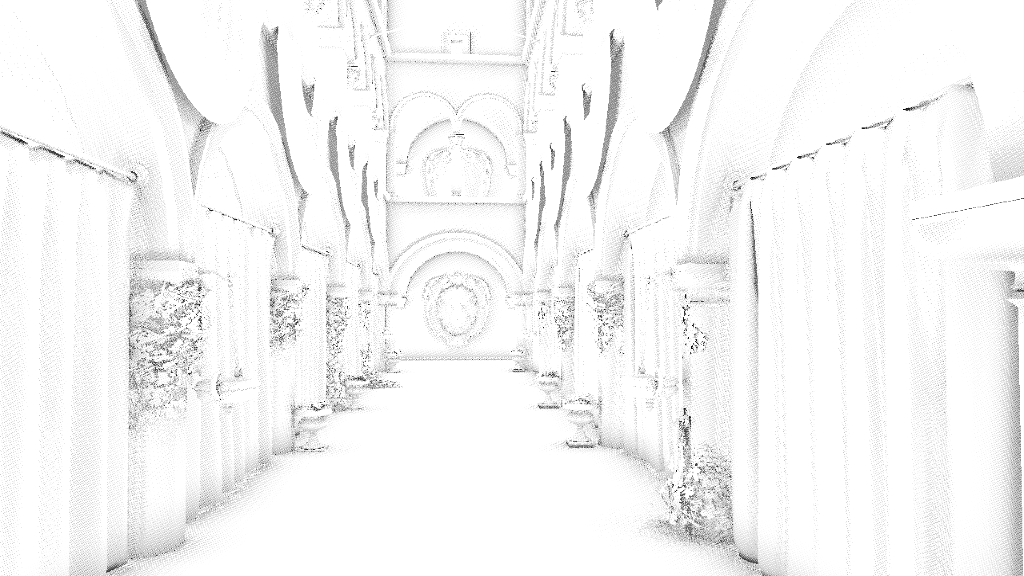
\includegraphics[width=0.48\textwidth]{figures/dbg_ao.png}\hfill%
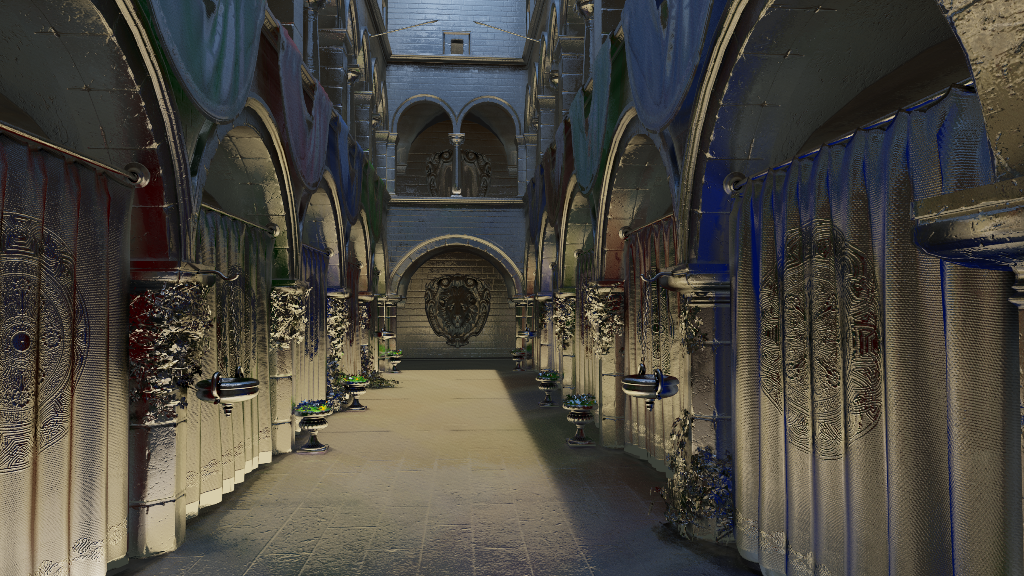
\includegraphics[width=0.48\textwidth]{figures/dbg_refl.png}

\vspace{5pt}

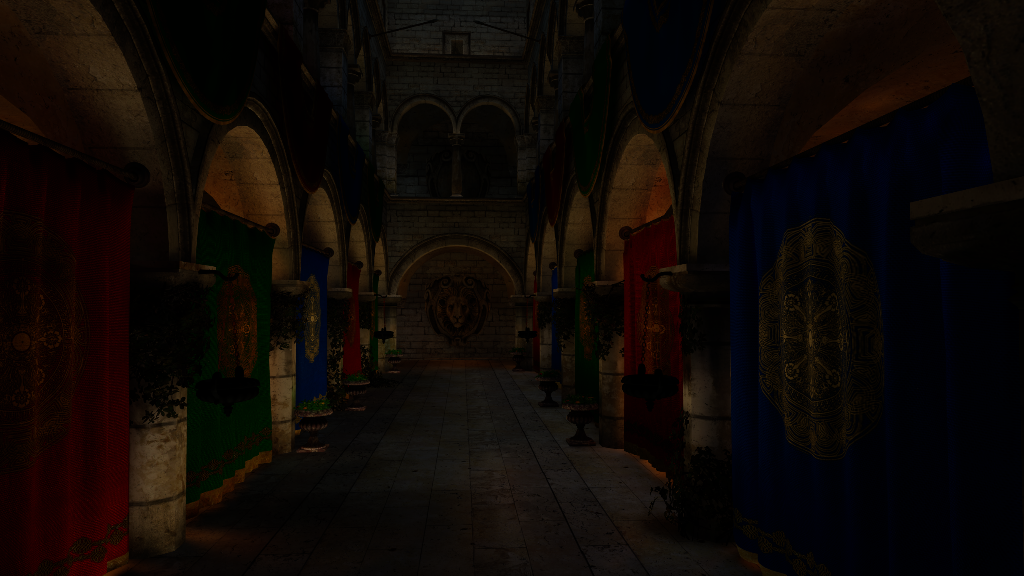
\includegraphics[width=0.48\textwidth]{figures/dbg_gi.png}\hfill%
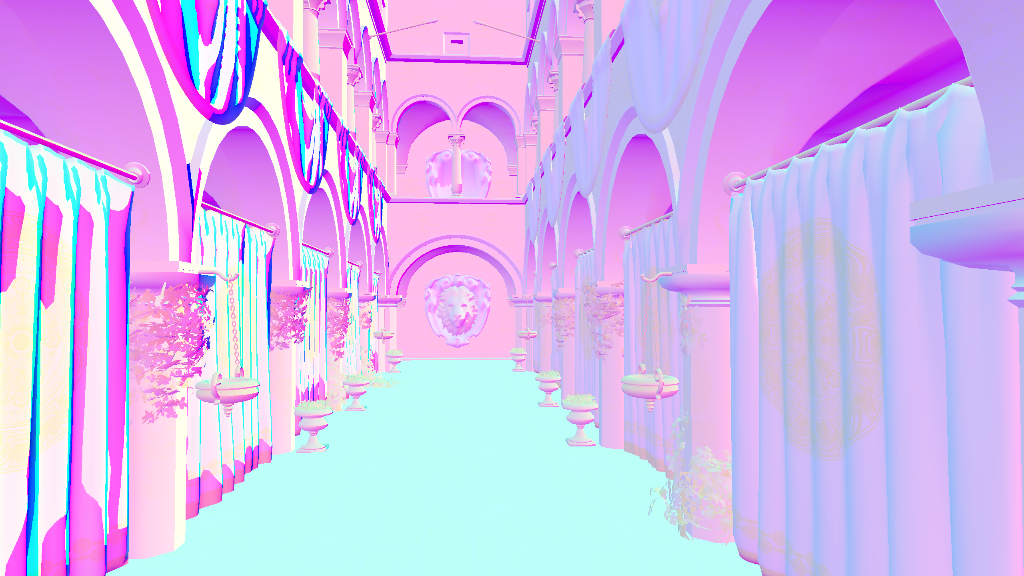
\includegraphics[width=0.48\textwidth]{figures/dbg_normals.png}
\caption[Pojedina\v{c}ni signali izolovani debug prikazom]{Pojedina\v{c}ni signali izolovani kroz \texttt{render.debugview}, ista scena i kamera: ambijentalna
okluzija (gore levo), reflektovana radijansa (gore desno), indirektni GI \v{c}lan (dole levo) i normale G-bafera
(dole desno). To su sirovi me\dj{}urezultati pre nego \v{s}to se u forward prolazu kombinuju,
a ne gotova slika.}
\label{fig:effect-gallery}
\end{figure}

Globalno osvetljenje je jedini od \v{c}etiri efekta koji znatno menja sliku.
Pojedina\v{c}no uklju\v{c}ivanje senki, ambijentalne okluzije ili refleksija pomera kona\v{c}nu sliku za prosek od
2.1 do 2.5 nivoa od 255 sa ovog gledi\v{s}ta, dok je globalno osvetljenje pomera za 23.9, faktor
deset. Bafer
ambijentalne okluzije je skoro beo preko ve\'ceg dela frejma jer je atrijum Sponze otvoren, pa je
okluzija ograni\v{c}ena na svodove arkada i podno\v{z}ja stubova. Sirovi GI \v{c}lan je u apsolutnom iznosu taman,
ali nosi preliv boja (crvene i zelene zavese koje boje kamen pored sebe) koji konstantan ambijent ne mo\v{z}e da reprodukuje.

\paragraph{Dva upozorenja ograni\v{c}avaju odnose izme\dj{}u proizvo\dj a\v{c}a.} Prvo je da oni nisu svojstva
\v{s}ejdera. Tri a-trous reda na Slici~\ref{fig:vendor-ratio} su jedan \v{s}ejder pokrenut tri puta sa
sve \v{s}irim korakom uzorkovanja, a odnos pada preko njih sa \perfAtrousGIFirst{} na \perfAtrousGILast{} na GI lancu (\perfAtrousAOFirst{} na \perfAtrousAOLast{} na AO). Kontrolisani
eksperiment na lancu denoisa senki, koji izvr\v{s}ava isti \v{s}ejder, razdvaja dve stvari
koje se razlikuju izme\dj{}u tih redova. Kad se jezgro dr\v{z}i uniformnim, a menja samo unutra\v{s}nja rezolucija, odnos izme\dj{}u prve i tre\'ce iteracije je \(1.02\) u punoj rezoluciji i \(0.47\) u polovini, a
sa jezgrom veli\v{c}ine penumbre je \(1.20\) i \(0.65\). Obe grane u punoj rezoluciji su ravne, a
obe grane u polovini rezolucije se invertuju, pa ga pokre\'ce rezolucija na kojoj lanac radi, a ne
jezgro, a uniformna grana u polovini rezolucije reprodukuje GI i AO lance (\(0.47\) naspram
\perfAtrousGIDrop{} i \perfAtrousAODrop{}, isti pad od prve do tre\'ce \v{c}itan iz osnovnih linija \texttt{+gi}). Za\v{s}to bi manji radni skup trebalo da obrne redosled proizvo\dj a\v{c}a ovde nije izolovano i
zahtevalo bi hardverske brojače, a ne timestampove. Eksperiment ipak utvr\dj{}uje da se odnos
proizvo\dj a\v{c}a po prolazu mora navoditi sa rezolucijom pri kojoj je izmeren, jer se isti kod
invertuje preko te jedne promenljive (tri pokretanja po grani, medijane, RX 9070 XT naspram RTX 5070).

Drugo ograni\v{c}ava sam argument o obilasku. Odeljak~\ref{sec:accel-pregled} nudi
petlju obilaska vo\dj enu \v{s}ejderom kao strukturni razlog da se o\v{c}ekuje da posao sa zracima ko\v{s}ta vi\v{s}e na RDNA,
a podela po prolazima je s tim u skladu, jer prolazi koji prate imaju prose\v{c}an odnos \perfVendorTracingMean{} naspram
\perfVendorOtherMean{} za sve ostale prolaze. To ipak ne obja\v{s}njava razliku celog frejma, a
lestvica to ka\v{z}e. RX 9070 XT je \perfLadderRatioShadows{} puta sporija od RTX 5070 na pre\v{c}ki \texttt{shadows}
i \perfLadderRatioGi{} puta sporija na \texttt{+gi}, pa se razlika \emph{smanjuje} kako se pra\'cenje zraka dodaje, a
sam posao sa pra\'cenjem zraka (ukupno \texttt{+gi} minus ukupno \texttt{rt-off}) nosi odnos od
\perfRtOnlyRatio{} naspram \perfLadderRatioBase{} za frejm bez pra\'cenja zraka. Da je obilazak vo\dj en \v{s}ejderom
dominantan \v{c}lan, dodavanje pra\'cenja zraka trebalo bi da pove\'ca razliku, a ne da je zatvara. Po\v{s}teno \v{c}itanje je
da je ovaj engine uop\v{s}te sporiji na ovoj AMD kartici iz razloga koje merenje ne identifikuje,
i da se kazna ne koncentri\v{s}e u pra\'cenju zraka. Pre\v{c}ka \texttt{rt-off} je najmanje
pouzdana od ovih vrednosti, sa \perfSpreadBaseAMD{}\% rasipanja izme\dj{}u pokretanja naspram \perfSpreadBaseNV{}\% na NVIDIA strani, iz
razloga datog u Odeljku~\ref{sec:metodologija}, iako trend pre\v{z}ivljava i bez nje, jer se dve
pre\v{c}ke sa obe njene strane rasipaju najvi\v{s}e \perfSpreadNeighbourMax{}\% na bilo kojoj kartici.

\section{Dve strategije senki: inline naspram stohasti\v{c}ke}
\label{sec:analiza-shadow-strategy}

Dve strategije senki iz Odeljka~\ref{sec:senke} imaju razli\v{c}ito oblikovane krive cene: podrazumevana
inline putanja prati dva zraka po svetlu po pikselu unutar forward \v{s}ejdera, dok stohasti\v{c}ka
bira jedno svetlo po pikselu resampliranim uzorkovanjem po zna\v{c}aju i rekonstrui\v{s}e rezultat zajedni\v{c}kim
denoiserom. Tabela~\ref{tab:shadow-strategy} meri obe na istoj sceni.

\begin{table}[tbp]
\caption[Cena inline naspram stohasti\v{c}kih senki]{Dve strategije senki na istoj sceni sa pet uklju\v{c}enih svetala (GPU ms, delta nad
\texttt{rt-off}).}
\label{tab:shadow-strategy}
\centering
\input{data/perf-shadow-strategy.tex}
\end{table}

\begin{figure}[tbp]
\centering
\begin{tikzpicture}
\begin{axis}[width=0.7\textwidth, height=6.0cm,
  xlabel={adapter}, ylabel={cena nad \texttt{rt-off} (GPU ms)},
  xtick={0,1}, xticklabels={RX 9070 XT, RTX 5070},
  xmin=-0.3, xmax=1.3, ymin=0, ymax=4,
  grid=major, grid style={black!12},
  tick label style={font=\small}, label style={font=\small},
  legend style={at={(0.02,0.98)}, anchor=north west, font=\small, draw=black!30}]
\addplot[thick, mark=*] table[x=i, y=inline] {data/shadow-strategy.dat};
\addplot[thick, mark=square*, dashed] table[x=i, y=stochastic] {data/shadow-strategy.dat};
\legend{inline, stochastic}
\end{axis}
\end{tikzpicture}
\caption[Cena strategije senki se obr\'ce izme\dj{}u proizvo\dj a\v{c}a]{Linije se seku. Na 9070 XT
stohasti\v{c}ka putanja je jeftinija, dok je na 5070 inline putanja jeftinija za faktor
\perfShadowRatioNV{}. Nijedan redosled se ne uop\v{s}tava.}
\label{fig:shadow-strategy}
\end{figure}

Dve kartice se ne sla\v{z}u oko toga koja je strategija jeftinija, a Slika~\ref{fig:shadow-strategy} pokazuje
kako se linije seku. Na RX 9070 XT stohasti\v{c}ka putanja pobe\dj uje,
\perfShadowStochAMD{} ms naspram \perfShadowInlineAMD{} ms. Na RTX 5070 jako gubi,
\perfShadowStochNV{} ms naspram \perfShadowInlineNV{} ms, faktor \perfShadowRatioNV{}.

Stohasti\v{c}ka putanja zamenjuje zrake po svetlu jednim zrakom uzorkovanim po zna\v{c}aju plus lancem
rekonstrukcije, \v{s}to menja broj zraka za cenu filtriranja, i isplati se upravo kad su zraci skupi u odnosu na
filtriranje. Na 5070 o\v{c}igledno nisu, jer pla\'canje temporalnog prolaza, tri à-trous
iteracije i upsample-a da bi se izbeglo deset koherentnih inline zraka ovde donosi neto gubitak, dok se na
9070 XT ista razmena isplati. Taj redosled je ono \v{s}to bi podela obilaska iz
Odeljka~\ref{sec:accel-pregled} predvidela, jer vo\dj enje obilaska iz instrukcija \v{s}ejdera \v{c}ini da
zrak konkuri\v{s}e \v{s}ejdingu za iste izvr\v{s}ne resurse, \v{s}to namenski hardver za obilazak ne \v{c}ini.
Dva merenja celog frejma po kartici ne mogu da razdvoje taj mehanizam od taktova, ke\v{s}a, rasporedjivanja
drajvera ili pona\v{s}anja samog lanca denoisa po proizvo\dj a\v{c}u, za koji ova glava pokazuje da se
invertuje sa rezolucijom. Inverzija je izmeren rezultat, a mehanizam je samo o\v{c}ekivano
obja\v{s}njenje za nju.

Izbor tehnike senki je stoga svojstvo ciljne arhitekture: renderer koji
fiksira bilo koju strategiju je pogre\v{s}an na jednoj od ove dve kartice, a evaluacija na jednom proizvo\dj a\v{c}u to
ne mo\v{z}e da vidi.

Dva upozorenja ograni\v{c}avaju tvrdnju. Cena stohasti\v{c}ke putanje je skoro nezavisna od broja svetala, dok
cena inline putanje raste sa njim, pa je pet svetala jedna ta\v{c}ka na dve krive koje se moraju
negde se\'ci, iako ova scena ne mo\v{z}e da poka\v{z}e gde. A stohasti\v{c}ki producent je eksperimentalan i podrazumevano isklju\v{c}en, sa poznatim
artefaktima pri kretanju kamere gde se dva ta\v{c}kasta svetla preklapaju, pa su ovo brojevi prototipa,
a ne tehnike spremne za isporuku.

\section{Broj zraka naspram kvaliteta i brzine}
\label{sec:raycount}

Broj GI zraka po pikselu menja se kroz ceo pipeline (denoiser i temporalno razre\v{s}avanje uklju\v{c}eni,
stabilizovano preko 90 frejmova, RX 9070 XT), uz ocenu kvaliteta rekonstrukcije naspram path-traced reference
i GPU vremena naspram broja zraka.

\begin{table}[htb]
\centering
\caption[Kvalitet i GPU cena GI u zavisnosti od broja zraka po pikselu]{Kvalitet i GPU cena GI kao funkcija
zraka po pikselu (denoiser i temporalno razre\v{s}avanje uklju\v{c}eni, RX 9070 XT). GPU ukupno je GI-only
konfiguracija sa ostala tri efekta isklju\v{c}ena, pa je manji frejm od ukupnog
\texttt{+gi} iz Tabele~\ref{tab:cena}: isto apsolutno pove\'canje je \rcGpuPct\% ovog
frejma i otprilike tre\'cina punog frejma sa \v{c}etiri efekta.}
\label{tab:raycount}
\input{data/raycount.tex}
\end{table}

Koleno kvaliteta le\v{z}i na jednom zraku po pikselu, iako ne zato \v{s}to dodatni zraci ne rade ni\v{s}ta. Prelazak
sa 1 na 8 zraka ko\v{s}ta \rcGpuPct\% vi\v{s}e GPU vremena (\rcGpuLow{} do \rcGpuHigh{} ms) i vra\'ca
\rcPsnrGain{} dB PSNR-a, uz FLIP koji se pomera sa \rcFlipLow{} na \rcFlipHigh{}. Obe razlike
prevazilaze pragove iz Tabele~\ref{tab:metrics}, pa je dobitak stvaran, a ne
\v{s}um, i nazvati ga \v{s}umom bi precenilo rezultat. Jedan zrak \v{c}ini radnom ta\v{c}kom kurs razmene:
osam puta ve\'ci bud\v{z}et zraka kupuje 0.2 dB, otprilike tri puta prag merenja,
za \rcGpuPct\% frejma. FLIP se tako\dj e ne pobolj\v{s}ava monotono du\v{z} merenja, rastu\'ci sa
0.1449 pri dva zraka na 0.1458 pri \v{c}etiri pre nego \v{s}to ponovo padne, pa redosled izme\dj{}u susednih
pode\v{s}avanja nije razre\v{s}en ni tamo gde su krajnje ta\v{c}ke. Denoiser i temporalna akumulacija ve\'c vra\'caju ve\'cinu dostupnog kvaliteta
iz jednog zraka, pa dodatni uzorci po pikselu nisu mesto gde bi trebalo da ode bud\v{z}et zraka ovog engine-a.
To je u skladu sa ciljem dizajna SVGF-a (prostorno-temporalno
filtriranje koje 1 uzorak po pikselu \v{c}ini upotrebljivim), a ne svojstvom specifi\v{c}nim za ovu
implementaciju. Slika~\ref{fig:spp-sweep} prikazuje sirovi \v{s}um koji ovo filtriranje maskira, snimljen
sa isklju\v{c}enim GI prostornim denoiserom, GI temporalnom akumulacijom i TAA, pri fiksnom ograni\v{c}enju od 30 frejmova.
Isklju\v{c}ivanje TAA \v{c}ini sliku po\v{s}tenom: TAA je i sam temporalni
akumulator, pa se sa njim uklju\v{c}enim snimak stabilizuje na istu glatko\'cu kao denoisirana slika i
broj zraka izgleda kao da uop\v{s}te ne pravi razliku.

Za kvantifikaciju je potrebna mera hrapavosti po pikselu. \emph{Visokofrekventna energija} slike defini\v{s}e se kao
srednja apsolutna razlika izme\dj{}u vertikalno susednih piksela njenog kanala sivih tonova,
$\frac{1}{(H-1)W}\sum_{y,x} |g_{y+1,x} - g_{y,x}|$, ra\v{c}unata na 8-bitnom tonemapiranom snimku. \v{S}um
je podi\v{z}e, zamu\'cenje spu\v{s}ta, a mo\v{z}e se ponovo izra\v{c}unati iz commitovanih slika. Sa uklju\v{c}enim TAA, jedan
zrak po pikselu i potpuno denoisirana slika oboje dobijaju 5.9, \v{s}to je merenje koje ka\v{z}e da
slika ne bi pokazala ni\v{s}ta. Sa isklju\v{c}enim TAA broj zraka se \v{c}isto razdvaja: \hfSppOne{}, \hfSppTwo{}, \hfSppFour{} i \hfSppEight{} za
jedan, dva, \v{c}etiri i osam zraka po pikselu, monotono se pribli\v{z}avaju\'ci referenci kako broj uzoraka
raste.

\begin{figure}[tbp]
\centering
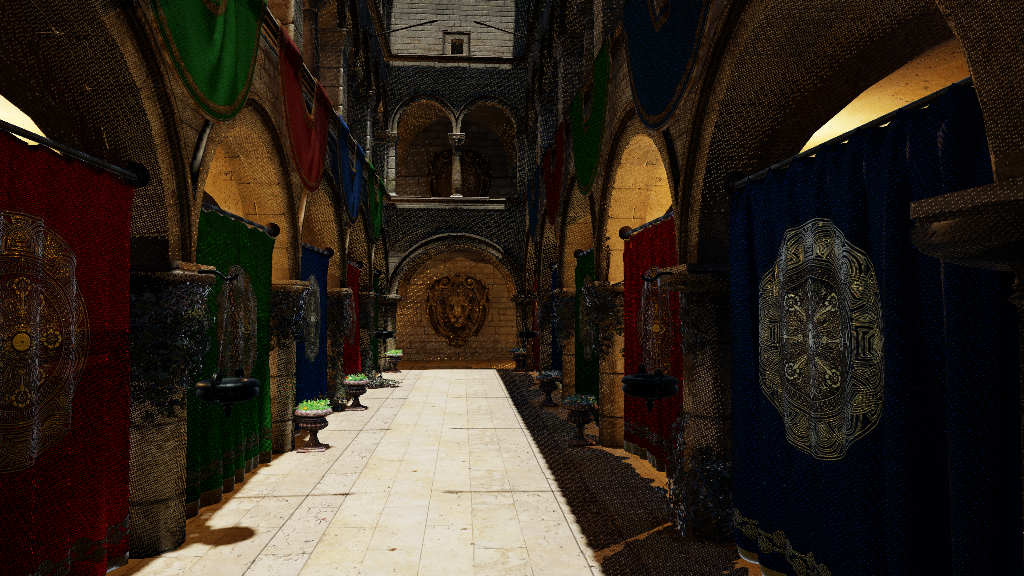
\includegraphics[width=0.48\textwidth]{figures/spp_sweep_1.png}\hfill%
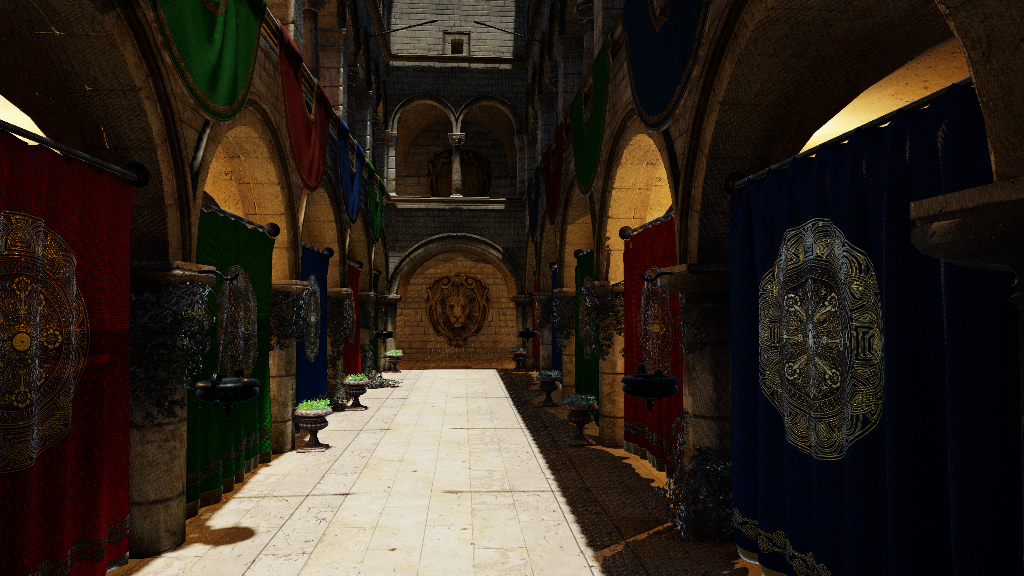
\includegraphics[width=0.48\textwidth]{figures/spp_sweep_8.png}
\caption[Sirovi GI \v{s}um pri jednom i osam zraka]{Uticaj zraka po pikselu na \v{s}um pre uklanjanja \v{s}uma, pre temporalnog razre\v{s}avanja i sa isklju\v{c}enim TAA
(GI; 1 zrak levo, 8 zraka po pikselu desno): vi\v{s}e zraka konvergira ka referenci uz
srazmerno vi\v{s}u cenu (Tabela~\ref{tab:raycount}).}
\label{fig:spp-sweep}
\end{figure}

\section{Polovina naspram pune rezolucije}
\label{sec:halfres}

Pra\'cenje dva hemisferna efekta prikupljanja u polovini rezolucije je najve\'ca pojedina\v{c}na odluka o ceni u
rendereru (Odeljak~\ref{sec:rendergraph}). Pode\v{s}avanje \texttt{render.gi.scale} i \texttt{render.ao.scale} na 1.0 isklju\v{c}uje je, ne menjaju\'ci ni\v{s}ta drugo, pa
se dve konfiguracije razlikuju u ta\v{c}no jednoj promenljivoj.

\begin{table}[tbp]
\caption[Pra\'cenje u polovini naspram pune rezolucije]{Polovina naspram pune rezolucije za GI i AO pra\'cenje (RX 9070 XT). Vreme je ukupno GPU vreme
konfiguracije \texttt{+gi}, a kvalitet je meren sa gledi\v{s}ta atrijuma naspram
konvergirane path-traced reference.}
\label{tab:halfres}
\centering
\input{data/halfres.tex}
\end{table}

Pra\'cenje u punoj rezoluciji ko\v{s}ta \hrDeltaMs{} ms vi\v{s}e po frejmu, pove\'canje od \hrDeltaPct\% na
bud\v{z}et od \hrHalfTotal{} ms, i vra\'ca \hrPsnrGain{} dB PSNR-a: dve konfiguracije su identi\v{c}ne
na drugoj decimali. SSIM i FLIP se pomeraju za 0.0008 i 0.0002, oba daleko unutar rasipanja
izme\dj{}u pokretanja. \v{C}itanje nije \rqt{puna rezolucija je malo bolja}, ve\'c \rqt{merenje ih ne
mo\v{z}e uop\v{s}te da razlikuje}.

Razlog je to \v{s}to je denoiser ograni\v{c}avaju\'ci \v{c}inilac, a ne mre\v{z}a uzoraka. Obe konfiguracije
hrane isti à-trous filter, \v{c}ije jezgro sa zaustavljanjem na ivicama ve\'c zamu\'cuje okolinu \v{s}iru od
faktora dva koji ih razdvaja, pa dodatne uzorke usrednjava upravo onaj filter koji \v{c}ini rezultat u
polovini rezolucije upotrebljivim. Obrazac polovina rezolucije plus bilateralni upsample stoga je
skoro besplatan, a ne kompromis kvaliteta prihva\'cen radi brzine.

Slika~\ref{fig:halfres-buffer} prikazuje sirovu GI iradijansu pod oba pode\v{s}avanja, snimljenu kroz
debug prikaz koji zaobilazi upsample, denoiser i kompoziciju. Bafer u polovini rezolucije nosi
44\% vi\v{s}e visokofrekventne energije po meri hrapavosti iz Odeljka~\ref{sec:raycount} (41.68
naspram 28.91). Ta mera je ponovljiva tamo gde razlika po pikselu nije: drugi
snimak u punoj rezoluciji sa identi\v{c}nim pode\v{s}avanjima daje 28.85, u okviru 0.2\%, a od
prvog se razlikuje za 18.3 nivoa sivog po pikselu samo zato \v{s}to su dva pra\'cenja izvukla razli\v{c}ite slu\v{c}ajne uzorke. Dakle
razlika od 35.4 po pikselu izme\dj{}u bafera u polovini i punoj rezoluciji je samo oko dvostruko ve\'ca od
praga izme\dj{}u pokretanja i nosi malo informacije, dok je razlika u hrapavosti daleko izvan njega. \v{C}etiri
puta vi\v{s}e zraka zaista daje merljivo \v{c}i\v{s}\'ci bafer, iako Tabela~\ref{tab:halfres} pokazuje da
ni\v{s}ta nizvodno od filtera to ne \v{c}uva.

\begin{figure}[tbp]
\centering
\begin{minipage}{0.48\textwidth}\centering
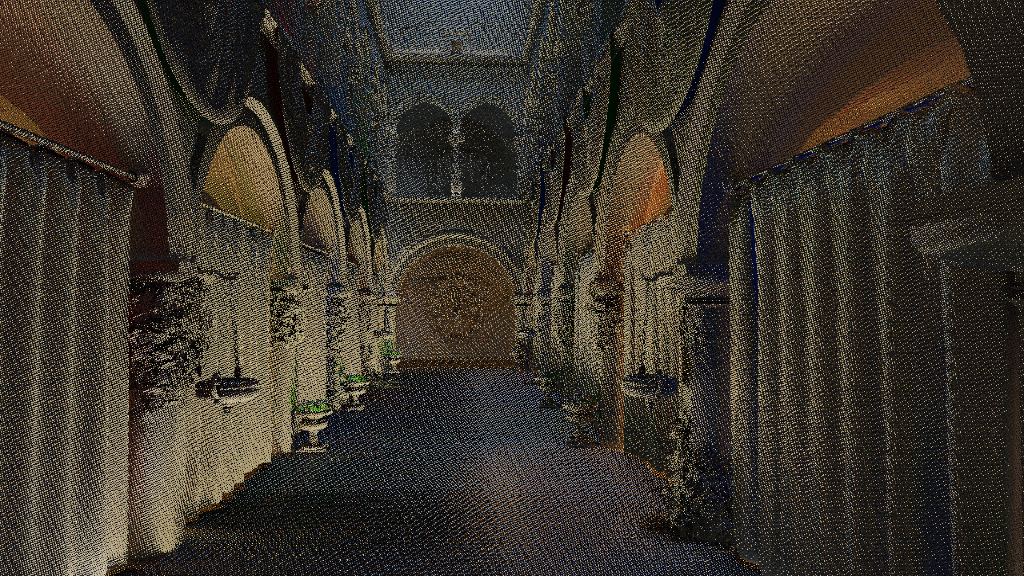
\includegraphics[width=\linewidth]{figures/gi_halfres.png}\\{\small pola (0.5)}
\end{minipage}\hfill
\begin{minipage}{0.48\textwidth}\centering
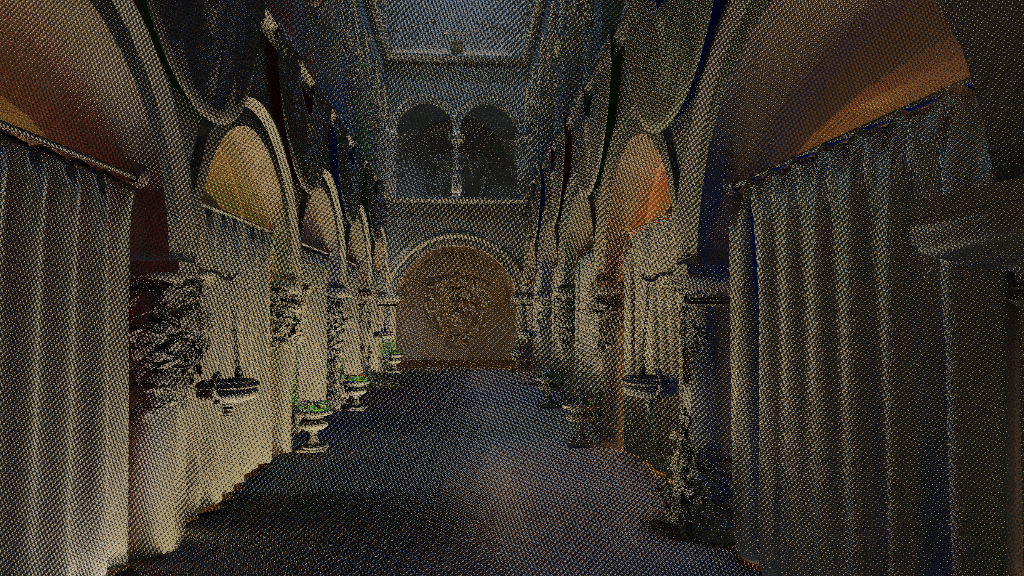
\includegraphics[width=\linewidth]{figures/gi_fullres.png}\\{\small puna (1.0)}
\end{minipage}
\caption[Sirovi GI bafer: polovina naspram pune rezolucije]{Sirovi GI bafer pre upsample-a i
denoisera, pri \texttt{render.gi.scale} 0.5 i 1.0 (\texttt{render.debugview} 6). Puna rezolucija daje
\v{s}iro zrno: 28.91 naspram 41.68 po meri visokofrekventne energije. U kona\v{c}noj slici ta
razlika se ne meri (Tabela~\ref{tab:halfres}).}
\label{fig:halfres-buffer}
\end{figure}

Dva upozorenja ograni\v{c}avaju tu tvrdnju. Vrednosti kvaliteta dolaze sa jednog gledi\v{s}ta, a ne iz prose\v{c}ne
vrednosti tri pogleda kori\v{s}\'cene drugde, a zaklju\v{c}ak je specifi\v{c}an za difuzne signale prikupljanja: kao \v{s}to
Odeljak~\ref{sec:rendergraph} obrazla\v{z}e, isti tretman primenjen na senke ili refleksije
uni\v{s}tio bi ta\v{c}no visokofrekventni detalj zbog kog ti efekti postoje, zbog \v{c}ega se nijedan
ne prati u polovini rezolucije.

\section{Evaluacija denoisera (SVGF)}
\label{sec:denoise-eval}

Sopstveni doprinos SVGF prostornog denoisera izoluje se dr\v{z}anjem temporalne akumulacije konstantnom
(uklju\v{c}ene u oba stanja, stabilizovano preko 90 frejmova) i ocenjivanjem ulaza sa \v{s}umom naspram denoisiranog
rezultata naspram path-traced reference, pri fiksna 2 zraka po pikselu, RX 9070 XT.

\begin{table}[htb]
\centering
\caption[Doprinos SVGF denoisera na mirnom frejmu]{Doprinos SVGF denoisera naspram
path-traced reference (2 zraka/piksel, temporalno razre\v{s}avanje uklju\v{c}eno u oba slu\v{c}aja). Dva reda se razlikuju
za manje od rasipanja ovih metrika izme\dj{}u pokretanja, pa ova tabela pokazuje da filter ne pravi \emph{nikakvu
merljivu razliku} na stabilizovanom mirnom frejmu, a ne da ga pogor\v{s}ava.}
\label{tab:denoise-eval}
\input{data/denoise-eval.tex}
\end{table}

Sa ve\'c aktivnom temporalnom akumulacijom, prostorni SVGF prolaz menja stati\v{c}ke metrike iz
Tabele~\ref{tab:denoise-eval}
(PSNR, SSIM, FLIP) za manje od \v{s}uma merenja, daleko unutar pragova iz
Tabele~\ref{tab:metrics}. Slika~\ref{fig:denoise-compare} pokazuje \v{s}ta ceo lanac rekonstrukcije
radi istom frejmu. Temporalna istorija radi u su\v{s}tini svu
vidljivu konvergenciju na ovom stabilizovanom frejmu, a doprinos samog filtera pokazuje se u temporalnoj
stabilnosti. RMS delta izme\dj{}u frejmova na istom mirnom pogledu (frejm $N$ naspram $N{+}1$ u
stabilnom stanju, proksi treperenja pri statičnoj kameri, a ne kretanje) pada sa \flickerOff{} sa
isklju\v{c}enim denoiserom na \flickerOn{} sa uklju\v{c}enim, smanjenje od \flickerPct\%. Taj proksi je jedini
broj stabilnosti specifi\v{c}an za denoiser ovde, i verovatno potcenjuje filter, jer stati\v{c}na kamera
ne mo\v{z}e da optereti temporalni. Odeljak~\ref{sec:motion} meri stabilnost kako treba pod kretanjem,
ali varira tehniku, a ne filter, pa ograni\v{c}ava ono \v{s}to ceo lanac rekonstrukcije
posti\v{z}e, a ne ono \v{s}to ovaj prolaz doprinosi. Smanjenje treperenja je osetljivo na
jedan detalj protokola: ako se temporalna istorija ne o\v{c}isti pre uzorkovanja, slu\v{c}aju bez filtera
se pripisuje \v{s}um nakupljen dok su se resursi jo\v{s} u\v{c}itavali, \v{s}to napuhuje prividno
smanjenje na blizu 40\%, pa snimci sa tim \v{c}i\v{s}\'cenjem i bez njega nisu uporedivi. GPU cena
denoisera \v{c}ita se iz njegovih sopstvenih timestamp opsega, a ne iz A/B celog frejma: tri
\texttt{GIDenoise} à-trous iteracije ukupno ko\v{s}taju \perfDenoiseAMD{} ms na 9070 XT i
\perfDenoiseNV{} ms na 5070 (Tabela~\ref{tab:pass-cost}), naspram bud\v{z}eta celog frejma blizu devet
milisekundi, a jeftine su delom jer rade u polovini rezolucije. Uklju\v{c}ivanje i isklju\v{c}ivanje denoisera
i oduzimanje ukupnih vrednosti celog frejma daje oko 0.07 ms, \v{s}to ne treba navoditi: manje je od
rasipanja izme\dj{}u pokretanja identi\v{c}ne konfiguracije, pa meri \v{s}um, a ne filter.

Debug prikazi 6 i 7 izoluju filter od svega ostalog na slici, prikazuju\'ci bafer GI iradijanse u polovini
rezolucije kakvog ga trace ostavlja i posle temporalne akumulacije plus à-trous, pre nego \v{s}to se
bilo koji upsample-uje ili kompozituje (Slika~\ref{fig:gi-denoise-ab}). Visokofrekventna energija definisana
u Odeljku~\ref{sec:raycount} pada sa \hfGiRaw{} na \hfGiDenoised{} izme\dj{}u ta dva, oko 96\% od
nje, dok srednji nivo raste jer filter popunjava piksele gde je svaki zrak slu\v{c}ajno
promašio.

Dakle filter skoro potpuno transformi\v{s}e me\dj{}ubafer, a ipak je kona\v{c}na slika
nepromenjena u okviru \v{s}uma merenja. Pipeline nizvodno upija taj posao: bafer se
upsample-uje iz polovine rezolucije, mno\v{z}i albedom povr\v{s}ine, dodaje direktnom osvetljenju koje mu dominira,
pa prolazi kroz temporalno razre\v{s}avanje koje je samo jak niskopropusni filter u vremenu. Pri dva zraka po pikselu sa
ve\'c aktivnom temporalnom akumulacijom, prostorni à-trous je skoro suvi\v{s}an za globalno
osvetljenje i gori nego suvi\v{s}an za refleksije, zbog \v{c}ega se za prvo zadr\v{z}ava na tri iteracije,
a za drugo isklju\v{c}uje, umesto da se primeni uniformno, i govori u prilog tome da se
bud\v{z}et rekonstrukcije prvo tro\v{s}i na temporalnoj, pa tek onda na prostornoj strani.

\paragraph{Isti filter \v{s}teti refleksijama.} Isti à-trous radi na signalu refleksija
i tamo se pokazao neto negativnim, zbog \v{c}ega je sada podrazumevano isklju\v{c}en: njegovo isklju\v{c}ivanje
pobolj\v{s}alo je svaku prostornu metriku odjednom, FLIP 0.1742 naspram 0.1746, PSNR 21.75 naspram 21.70, SSIM
0.6473 naspram 0.6419. To \v{s}to se sve tri pomeraju u istom smeru razlikuje ovo od igranja metrikama,
jer je potpis puko uklanjanja zamu\'cenja to da se FLIP i PSNR pobolj\v{s}avaju dok SSIM pada. Strukturni
razlog je to \v{s}to filter vode normala i dubina povr\v{s}ine koja prima, \v{s}to je ispravno
za difuzno prikupljanje, a pogre\v{s}no za refleksije: reflektovana radijansa zavisi od pogleda, pa su na
ravnoj reflektuju\'coj povr\v{s}ini te vodilje konstantne i jezgro se \v{s}iroko otvara upravo tamo gde reflektovani
detalj \v{z}ivi. Lanac je radio u punoj rezoluciji bez upsample-a posle sebe, pa njegovo uklanjanje izbacuje
lanac prolaza u punoj rezoluciji iz cene refleksija u
Tabeli~\ref{tab:cena}. Jezgro vo\dj eno hrapavo\v{s}\'cu ostaje strukturno ispravno re\v{s}enje, iako sada
mora da pobedi isklju\v{c}eno filtriranje, a ne tri iteracije.

\paragraph{Cena filtera nije ista kod oba proizvo\dj a\v{c}a.} Odmotavanje spoljne petlje à-trous, u\v{c}injeno da bi se
smanjio pritisak na registre \v{s}ejdera (Odeljak~\ref{sec:occupancy}), isplatilo se asimetri\v{c}no: na RTX
5070 je svaki korak postao br\v{z}i, dok je na RX 9070 XT bilo pribli\v{z}no nule na lancima GI i AO u polovini rezolucije
(prva iteracija sporija, poslednja br\v{z}a), a isplatilo se samo na lancima u punoj rezoluciji.
Tabela po prolazima pokazuje ostatak: AMD lanac denoisa je optere\'cen na po\v{c}etku (\texttt{GIDenoise0}
\perfGiDenoiseFirstAMD{} ms pada na \perfGiDenoiseLastAMD{} ms pri \texttt{GIDenoise2}), dok se NVIDIA obr\'ce (\perfGiDenoiseFirstNV{} ms raste na
\perfGiDenoiseLastNV{} ms). To je ista asimetrija zavisna od rezolucije izolovana u Odeljku~\ref{sec:cena}, vi\dj ena
s druge strane, a lokalnost naspram zauzetosti pri u\v{z}em koraku je o\v{c}igledna poluga. Kao
tamo, timestampovi je ne mogu razdvojiti od alternativa, a za to su potrebni brojači memorije
koje ovaj rad ne meri. Ono \v{s}to brojevi utvr\dj uju je prakti\v{c}na poenta: optimizacija \v{s}ejdera
opravdana brojem registara nije automatski dobitak i mora se meriti po proizvo\dj a\v{c}u kao sve ostalo u ovoj glavi.

\begin{figure}[tbp]
\centering
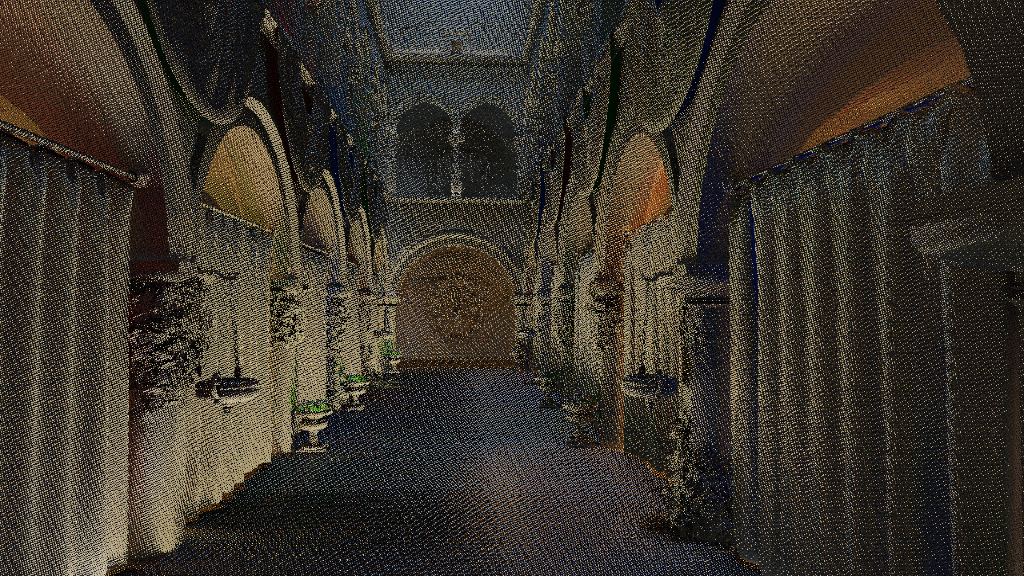
\includegraphics[width=0.48\textwidth]{figures/dbg_gi_raw.png}\hfill%
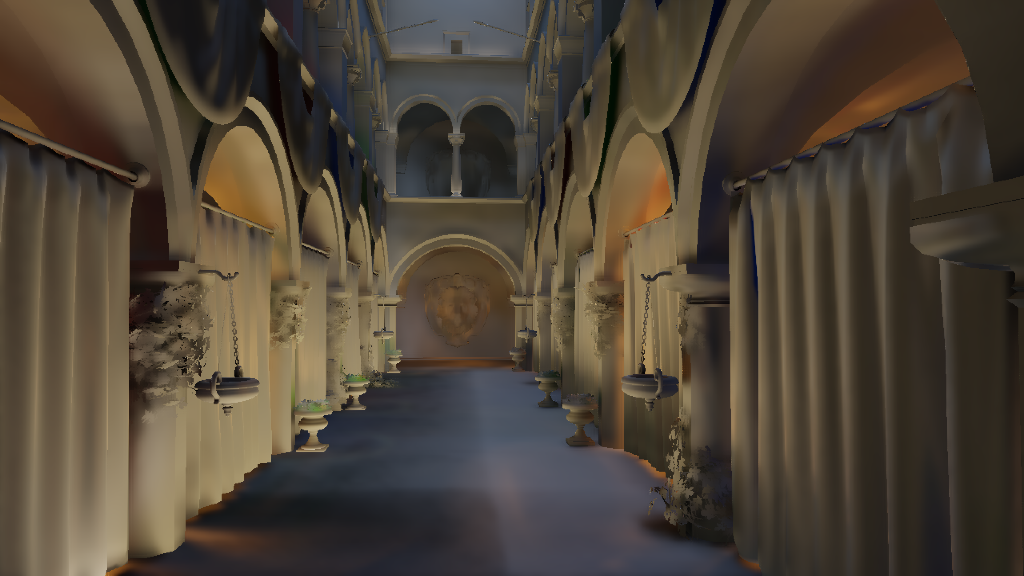
\includegraphics[width=0.48\textwidth]{figures/dbg_gi_denoised.png}
\caption[GI iradijansa pre i posle rekonstrukcije]{GI iradijansa u polovini rezolucije pre (levo) i posle (desno) temporalne akumulacije i
a-trous filtera, pre upsample-a i kompozicije (\texttt{render.debugview} 6 i 7). Levo je
zrnasti signal od jednog zraka, desno isti bafer posle rekonstrukcije.}
\label{fig:gi-denoise-ab}
\end{figure}

\begin{figure}[tbp]
\centering
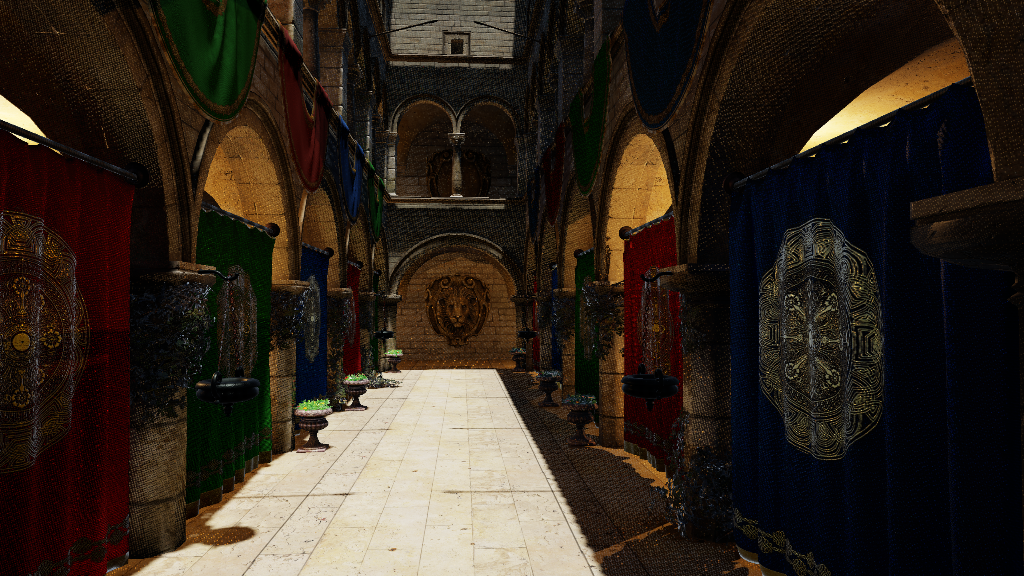
\includegraphics[width=0.62\textwidth]{figures/denoise_compare_noisy.png}

\vspace{5pt}

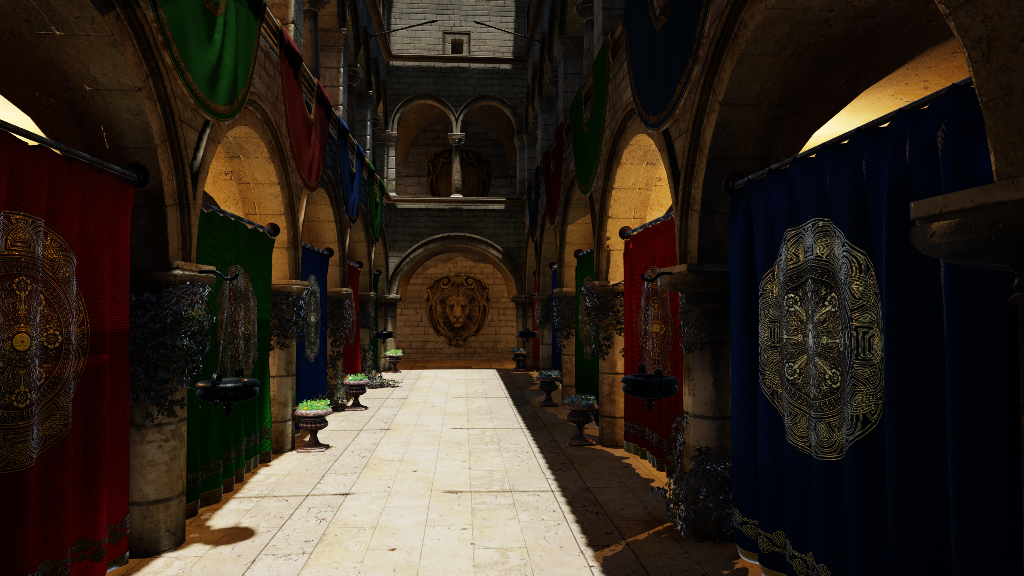
\includegraphics[width=0.62\textwidth]{figures/denoise_compare_denoised.png}

\vspace{5pt}

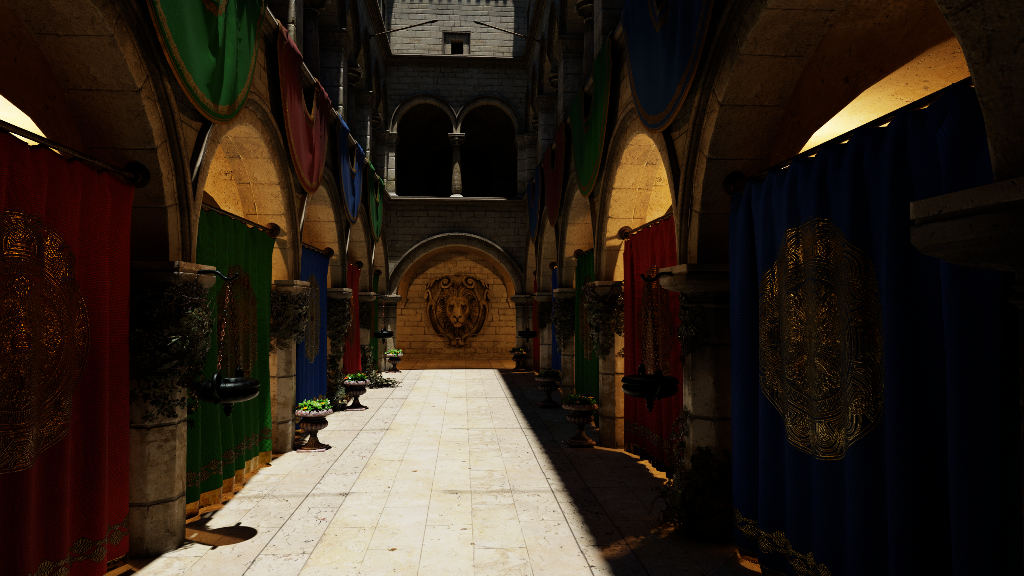
\includegraphics[width=0.62\textwidth]{figures/denoise_compare_reference.png}
\caption[Sirovi signal, rekonstrukcija i referenca]{Rekonstrukcija pri 2 zraka po pikselu: sirovi signal sa isklju\v{c}enim denoiserom, temporalnim razre\v{s}avanjem i TAA
(gore), pun rezultat u realnom vremenu sa sva tri uklju\v{c}ena (sredina) i path-traced
referenca (dole). Razlika od gornje do srednje je doprinos cele rekonstrukcije, dok je
sopstveni doprinos denoisera izolovan metrikama u tekstu, gde se pokazuje prvenstveno u temporalnoj
stabilnosti.}
\label{fig:denoise-compare}
\end{figure}

\section{Poređenje sa postoje\'cim re\v{s}enjima}
\label{sec:poredjenje}

Engine implementira rasterske screen-space osnovne linije za ambijentalnu okluziju i refleksije (SSAO, SSR;
Odeljak~\ref{sec:efekti}), pa je poređenje sa re\v{s}enjima prikazanim u
Glavi~\ref{ch:pregled} A/B na istoj sceni sa istom kamerom, koje izla\v{z}e slu\v{c}ajeve s kojima screen-space metoda
strukturno ne mo\v{z}e da izađe na kraj: okludere i reflektore van ekrana i disokluziju
(Slika~\ref{fig:rt-vs-ss}). Pozicioniranje naspram produkcijskih sistema (Lumen, RTXGI, ReSTIR) je
kvalitativno: doprinos je integrisana, izmerena, otvoreno licencirana implementacija sa ray query-jem,
a ne sistem koji nadma produkcijsko re\v{s}enje za globalno osvetljenje.

\begin{table}[tbp]
\caption[Kvalitet svake tehnike naspram reference]{Kvalitet svake tehnike naspram path-traced reference (usrednjeno preko tri gledi\v{s}ta:
atrijum, pod, galerija; RX 9070 XT). Ni\v{z}i FLIP i vi\v{s}i PSNR/SSIM su bolji.}
\label{tab:quality}
\centering
\input{data/quality.tex}
\end{table}

\begin{figure}[tbp]
\centering
\begin{tikzpicture}
\begin{axis}[width=0.88\textwidth, height=6.2cm,
  ylabel={FLIP $\downarrow$}, ymin=0, ymax=0.58,
  xtick={0,...,9},
  xticklabels={raster,SSAO,RT AO,SSR,RT refl.,RT shad.,RT shad. stoch.,SSGI,RT GI,all-RT},
  xticklabel style={font=\small, rotate=25, anchor=north east},
  tick label style={font=\small}, label style={font=\small},
  grid=major, grid style={black!12}, enlarge x limits=0.08]
\addplot[only marks, mark=*, mark size=2pt, black,
  error bars/.cd, y dir=both, y explicit]
  table[col sep=tab, x=i, y=flip, y error plus expr=\thisrow{hi}-\thisrow{flip},
        y error minus expr=\thisrow{flip}-\thisrow{lo}] {data/quality-spread.dat};
\end{axis}
\end{tikzpicture}
\caption[FLIP po tehnici sa rasipanjem preko gledi\v{s}ta]{Isti podaci kao
Tabela~\ref{tab:quality}, sa opsegom preko tri gledi\v{s}ta umesto samog proseka.
Trake su varijacija sadr\v{z}aja, a ne gre\v{s}ka merenja: govore da kadriranje pomera ocenu vi\v{s}e nego
ve\'cina ovih tehnika, pa dve preklopljene trake nisu dve nerazlu\v{c}ive
tehnike. Ponovljivost je otprilike 0.0024 FLIP, daleko u\v{z}a od bilo koje ovde nacrtane trake, pa su
razlike izme\dj{}u grupisanih ta\v{c}aka stvarne \v{c}ak i kad im se opsezi skoro potpuno preklapaju.
Rasipanje je i samo deo rezultata: raster ide od \qRasterFlipLo{} do \qRasterFlipHi{}
zavisno od kadriranja, dok RT GI ostaje u \qRtGiFlipLo{}--\qRtGiFlipHi{}. Tehnike koje
re\v{s}avaju indirektno osvetljenje su ta\v{c}nije u proseku i ujedna\v{c}enije preko scene, \v{s}to
sam prosek ne pokazuje.}
\label{fig:quality-spread}
\end{figure}

Naspram path-traced reference (Tabela~\ref{tab:quality}, sa rasipanjem po gledi\v{s}tu na
Slici~\ref{fig:quality-spread}) globalno osvetljenje je dominantna
poluga kvaliteta: sam RT GI podi\v{z}e
PSNR sa \qRasterPsnr{} (raster) na \qRtGiPsnr{} i smanjuje FLIP za vi\v{s}e od dve tre\'cine, a uklju\v{c}ivanje
svih efekata dosti\v{z}e FLIP \qAllRtFlip{}, PSNR \qAllRtPsnr{}, SSIM \qAllRtSsim{}, daleko najbli\v{z}e
referenci.

\paragraph{Gde je dobitak i \v{s}ta ekspozicija ima s tim.} Scena je tamna:
\exDarkShare\% piksela reference je ispod desetine pune luminanse, sa medijanom od
\exMedianLuma{}, jer su sunce i \v{c}etiri baklje jedina uklju\v{c}ena svetla, a tri
definisana reflektora kroz prozore Sponze su isklju\v{c}ena. To name\'ce prigovor da je dobitak dva renderovanja
koja se sla\v{z}u oko tame. Referenca je path trace iste scene sa istom ekspozicijom, pa
samo poređenje nije zahva\'ceno, ali VELI\v{C}INA dobitka jeste. Ponovno ocenjivanje gledi\v{s}ta atrijuma
na sve svetlijim podskupovima reference (maskiranje na referenci, nikad na tehnici,
\v{s}to bi dozvolilo tehnici da bira sebi povoljne piksele) menja dobitak od rastera do all-RT
sa \exLiftAll{} dB preko celog frejma na \exLiftLit{} dB preko najsvetlijih \exLitShare\%. Raster je
ono \v{s}to se pomera: ide sa \exRasterAll{} dB na \exRasterLit{} dB kako se tamni pikseli odbacuju, dok
se rezultat sa pra\'cenjem zraka jedva menja. Rasterizacija je skoro ta\v{c}na svuda gde svetlost stiže
direktno i zaostaje svuda gde ne stiže, pa se prednost koncentri\v{s}e u indirektno osvetljenom
delu frejma. Tu je mesto gde ova \v{c}etiri efekta treba da budu bitna, a koncentracija je
o\v{c}ekivani potpis, a ne artefakt, ali to zna\v{c}i da je naslovni iznos u decibelima
svojstvo ove ekspozicije koliko i tehnika, a svetlija scena bi prijavila manji.

Na ovim
metrikama celog frejma screen-space i ray-traced AO i refleksije su skoro izjedna\v{c}eni (SSAO naspram RT AO,
i SSR naspram RT refleksija, razlikuju se za manje od 0.01 u FLIP-u), jer su doprinosi okluzije i refleksije
mali na nivou celog frejma. Snimljen kroz debug prikaz koji izoluje samo
AO \v{c}lan, gledi\v{s}te atrijuma ima medijanu AO
od 255 od 255, tj. nikakvu okluziju, a samo 14.1\% (SSAO) i 17.6\% (RT AO) piksela pada
ispod 240. Efekat koji ostavlja pet \v{s}estina frejma netaknutim ne mo\v{z}e mnogo da pomeri prosek celog frejma,
kako god da se ra\v{c}una. Prednost pra\'cenja zraka je ta\v{c}nost van ekrana, koju prosek celog frejma
ne izoluje. Slike~\ref{fig:ssvsrt-ao} i~\ref{fig:ssvsrt-refl} je izoluju
za AO i za refleksije prikazuju\'ci same te bafere umesto kompozitovanog frejma.

\v{C}itana naspram cena, tri efekta se \v{c}isto razdvajaju, a razdvajanje je u dobitku,
a ne u ceni (Slika~\ref{fig:tradeoff}). Svaki od njih zaista pobolj\v{s}ava frejm u odnosu na \v{c}istu
rasterizaciju, za 0.0205 FLIP kod RT AO i 0.0122 kod RT refleksija naspram praga merenja od
0.0024, pa nijedan ne radi ni\v{s}ta. Ali pitanje s kojim se renderer zaista suo\v{c}ava je da li
ray-traced verzija zaslu\v{z}uje svoj multiplikator nad screen-space verzijom, a tu se odgovori razlikuju za
red veli\v{c}ine dok se cene ne razlikuju.

Na metrikama celog frejma prednost pra\'cenja zraka je stoga odlu\v{c}uju\'ca za globalno osvetljenje,
marginalna za refleksije i nerazre\v{s}ena za ambijentalnu okluziju. Taj redosled je svojstvo
metrike koliko i tehnika, iz gore datog razloga, a izolovani baferi ispod pokazuju
razlike koje kompozitovani prosek ne mo\v{z}e. Ali pravac vredi navesti jasno, umesto da se
prepusti \v{c}itaocu: ova evaluacija pokazuje vrednost pra\'cenja zraka za indirektno difuzno
osvetljenje, a ne pokazuje je za okluziju.

\begin{figure}[tbp]
\centering
\begin{tikzpicture}
% Log y: the three gains span 73x (0.0027 to 0.1978), so on a linear axis two of the three sit on the
% x-axis, indistinguishable from each other and from the measurement floor. The floor is the point of
% the figure, since AO clears it by 12% and reflections by 2.9x, and only a log axis shows that.
\begin{axis}[width=0.82\textwidth, height=6.4cm,
  xlabel={cena pra\'cenja zraka, kao umno\v{z}ak screen-space metode},
  ylabel={FLIP dobijen preko nje}, ymode=log,
  ymin=0.0018, ymax=0.42, xmin=1.35, xmax=3.7,
  ytick={0.002,0.005,0.01,0.02,0.05,0.1,0.2},
  yticklabels={0.002,0.005,0.01,0.02,0.05,0.10,0.20},
  grid=major, grid style={black!12},
  tick label style={font=\small}, label style={font=\small}]
\draw[dashed, black!55] (axis cs:1.35,0.0024) -- (axis cs:3.7,0.0024);
\node[font=\scriptsize, black!55, anchor=south east] at (axis cs:3.68,0.0024)
  {prag merenja};
% Segments, markers and label positions all come from data/tradeoff-seg.dat and data/tradeoff.dat
% (tools/gen_perf_plots.py), so they cannot drift from the ladder numbers.
\addplot[black!55, line width=1.1pt] table[col sep=tab, x=mult, y=flipGain] {data/tradeoff-seg.dat};
\addplot[only marks, mark=*, mark size=2.2pt, black] table[col sep=tab, x=mult, y=flipGain] {data/tradeoff-seg.dat};
\addplot[only marks, mark=none, font=\small, nodes near coords, point meta=explicit symbolic,
  every node near coord/.style={anchor=south, yshift=4pt}]
  table[col sep=tab, x=mid, y=flipGain, meta=effect] {data/tradeoff.dat};
\end{axis}
\end{tikzpicture}
\caption[\v{S}ta pra\'cenje zraka ko\v{s}ta naspram \v{s}ta vra\'ca]{\v{S}ta pra\'cenje zraka ko\v{s}ta naspram \v{s}ta
vra\'ca, po efektu. Svaki segment obuhvata umno\v{s}ke cene dva adaptera pri dobitku
kvaliteta tog efekta, koji je meren samo na RX 9070 XT, a isprekidana linija je prag merenja iz
Odeljka~\ref{sec:metodologija}. Cene su sve sli\v{c}ne, izme\dj{}u \perfSsFactorMin{} i \perfSsFactorMax{} puta screen-space
metode, a dobici nisu: globalno osvetljenje je za red veli\v{c}ine iznad druga dva,
a ambijentalna okluzija pada na prag. Obe ose se ra\v{c}unaju
unutar jednog para screen-space/ray-traced, odnos i razlika, pa nijedna ne zavisi od toga na kojoj
konfiguraciji par le\v{z}i i razli\v{c}ite osnovne linije dva gejta ne moraju da se sla\v{z}u.}
\label{fig:tradeoff}
\end{figure}

\begin{figure}[tbp]
\centering
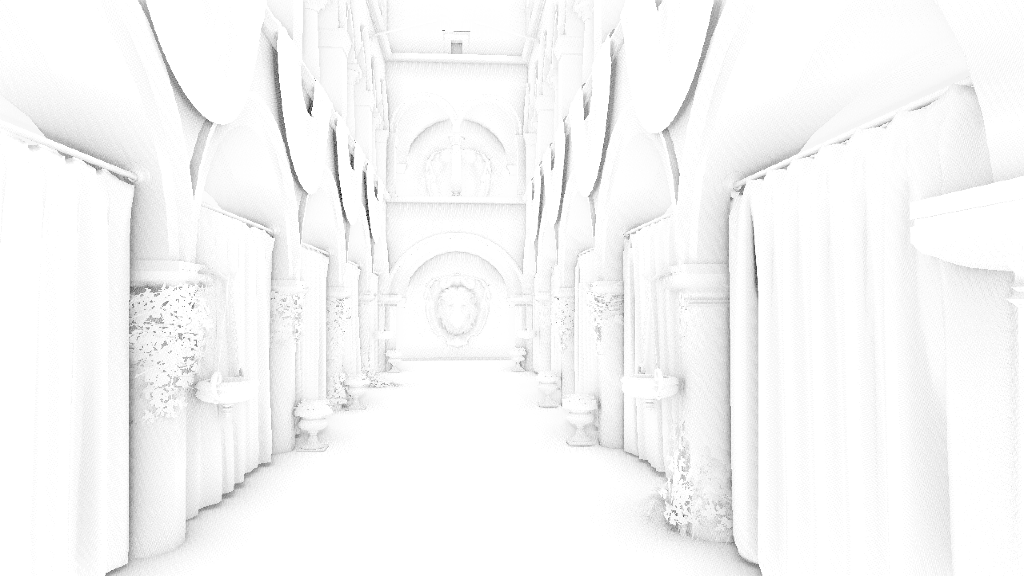
\includegraphics[width=0.485\textwidth]{figures/ssvsrt_ssao.png}\hfill
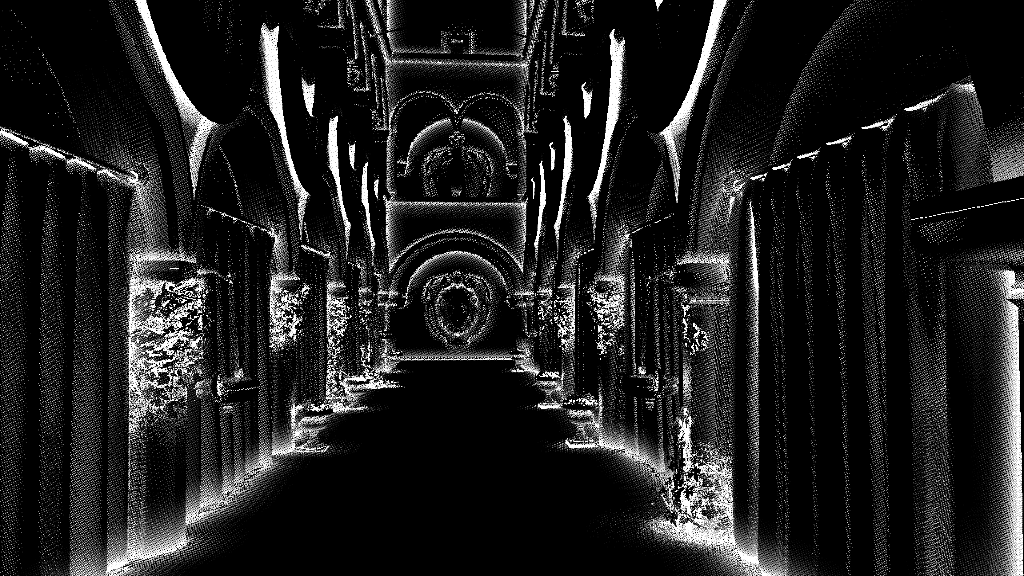
\includegraphics[width=0.485\textwidth]{figures/ssvsrt_rtao.png}
\caption[Screen-space naspram ray-traced ambijentalne okluzije]{Izolovani \v{c}lan okluzije sa gledi\v{s}ta
atrijuma, SSAO (levo) naspram ray-traced AO (desno). Oba panela prikazuju $1-\mathrm{AO}$ sa pojačanjem
4, ista transformacija na obe strane, pa je svetlo okludirano i skoro beli sirovi baferi postaju
\v{c}itljivi. SSAO razre\v{s}ava samo tanak obod gde se dve povr\v{s}ine sastaju u baferu dubine, \v{s}to je sve \v{s}to
mo\v{z}e da vidi, dok pra\'ceni \v{c}lan daje zavesama, svodovima i li\v{s}\'cu okluziju sa telom,
jer okludiraju\'ca geometrija ne mora biti na ekranu. \v{C}itati strukturno, a ne po pikselu: sirovi
stohasti\v{c}ki bafer se ne reprodukuje bit po bit, a dva snimka jedne konfiguracije razlikuju se za
prosek od 3.8 od 255 naspram 8.8 izme\dj{}u tehnika.}
\label{fig:ssvsrt-ao}
\end{figure} Dva producenta senki su tako\dj e skoro izjedna\v{c}ena ovde, \qRtShadowFlip{} za inline putanju naspram
\qMegalightsFlip{} za stohasti\v{c}ku, \v{s}to uti\v{c}e na to kako treba \v{c}itati Odeljak~\ref{sec:analiza-shadow-strategy}:
strategije se u terminima slike ne razlikuju statisti\v{c}ki, pa je inverzija proizvo\dj a\v{c}a
prona\dj ena tamo \v{c}ist rezultat cene, a ne kompromis kvaliteta.
Screen-space GI le\v{z}i izme\dj{}u ta dva nivoa: njegov FLIP (\qSsgiFlip{}) je znatno bolji od
AO/refleksijskih parova, ali daleko od RT GI (\qRtGiFlip{}), u skladu sa tim da SSGI prikuplja odbijenu
svetlost samo iz geometrije na ekranu, dok RT GI dopire i do povr\v{s}ina van ekrana i iza kamere.

\begin{figure}[tbp]
\centering
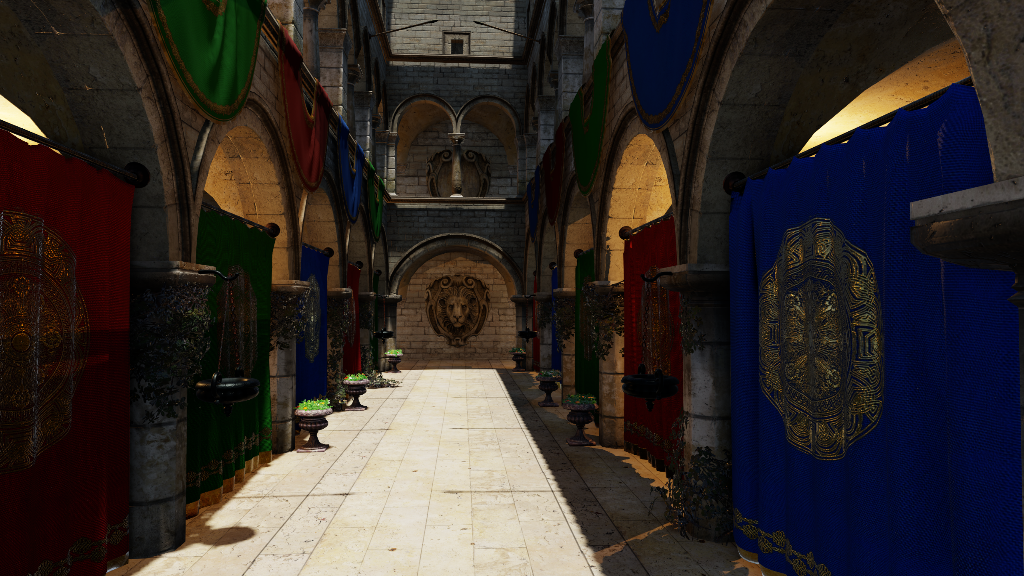
\includegraphics[width=0.48\textwidth]{figures/ss_all.png}\hfill%
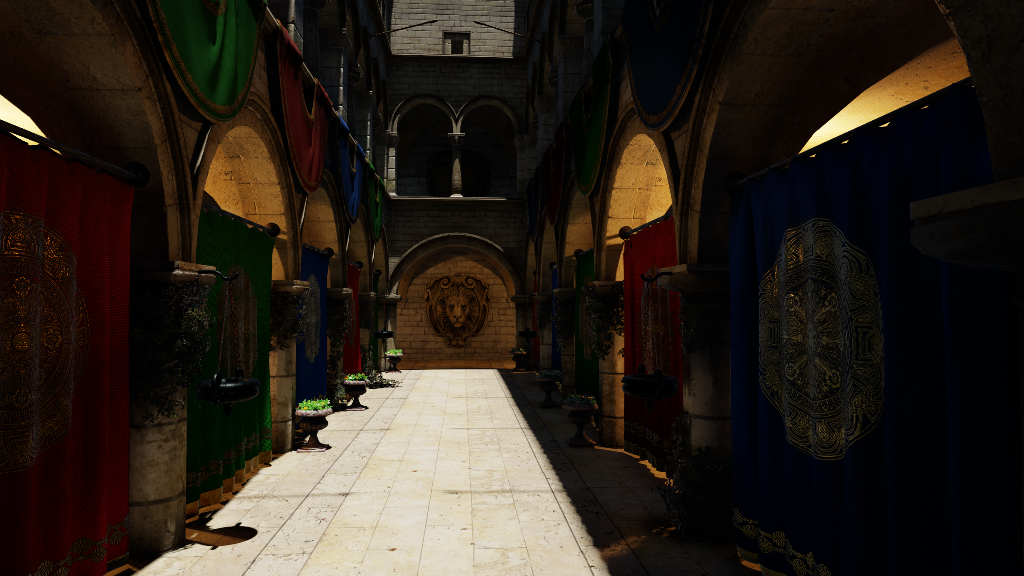
\includegraphics[width=0.48\textwidth]{figures/rt_all.png}
\caption[Screen-space naspram ray-traced konfiguracije]{Ista scena i kamera u dve kompletne
konfiguracije: screen-space (levo: mapa senki, SSAO, SSR, SSGI) naspram ray-traced (desno: pra\'cene
senke, RTAO, RT refleksije, RT GI). Senke prate ostatak jer screen-space nema parnjaka
pra\'cenoj senci, pa je mapa ono \v{s}to ta porodica zaista koristi. To je ista podela koju koristi red
\rqt{all-RT} Tabele~\ref{tab:quality}. Screen-space varijanta je svetlija jer ne
mo\v{z}e da oduzme svetlost koja stiže iz geometrije van ekrana.}
\label{fig:rt-vs-ss}
\end{figure}

\begin{figure}[tbp]
\centering
\begin{minipage}{0.48\textwidth}\centering
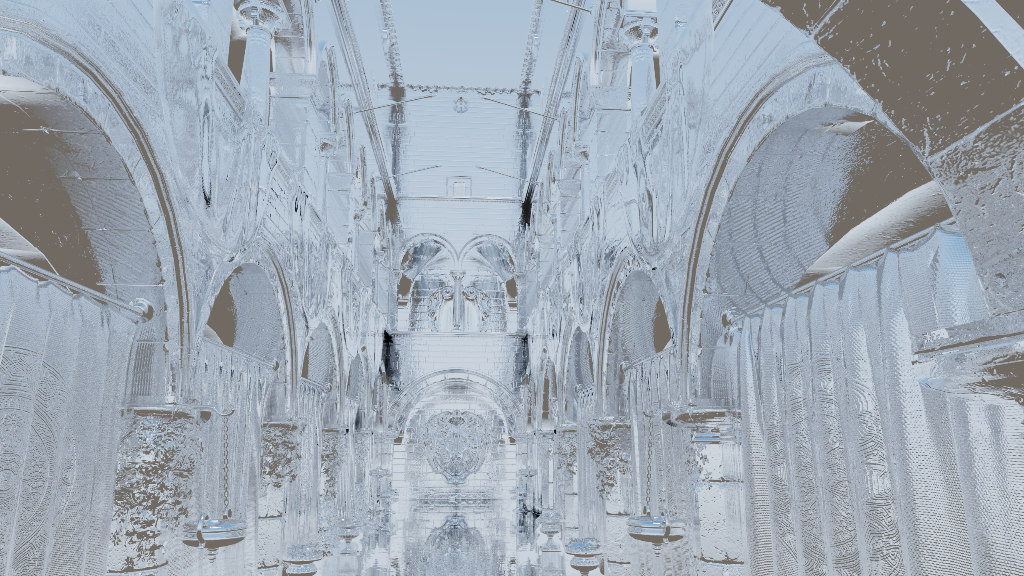
\includegraphics[width=\linewidth]{figures/ssvsrt_ssr.png}\\{\small SSR}
\end{minipage}\hfill
\begin{minipage}{0.48\textwidth}\centering
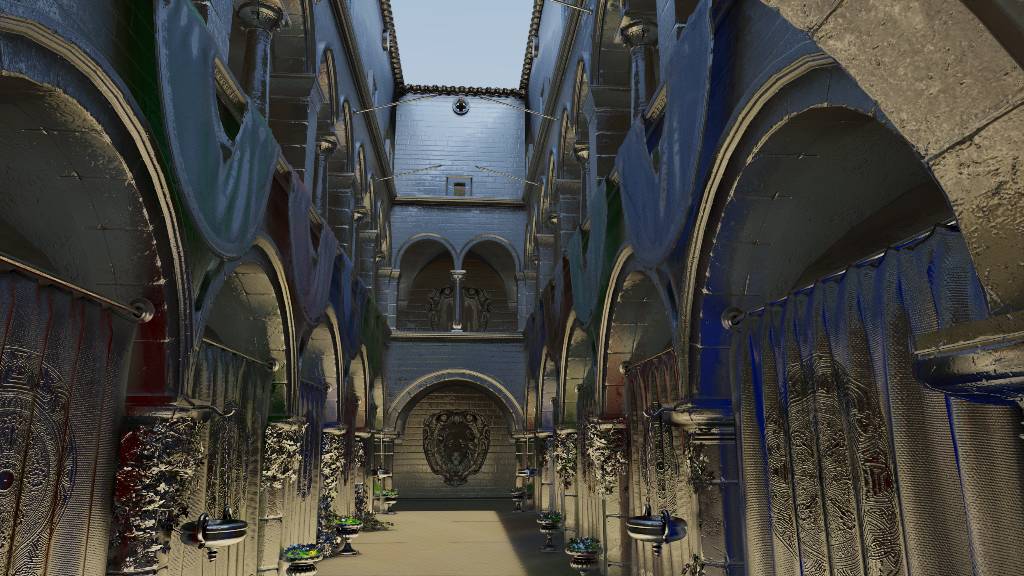
\includegraphics[width=\linewidth]{figures/ssvsrt_rtrefl.png}\\{\small RT refleksije}
\end{minipage}
\caption[Sirovi bafer refleksija: SSR naspram RT]{Sirovi bafer refleksija (\texttt{render.debugview}
3), isto gledi\v{s}te i iste podrazumevane vrednosti. SSR i RT pi\v{s}u u isti bafer, pa je izvor
refleksije jedina promenljiva. Kad marš kroz bafer dubine ne na\dj e ni\v{s}ta, SSR se vra\'ca na prefiltriranu
mapu okoline: 9.0\% piksela je zbog toga skoro belo, naspram 0.0\% desno, a
srednja vrednost bafera je 169.4 naspram 65.99. U kompozitovanom frejmu ta razlika se gubi pod direktnim
osvetljenjem, zbog \v{c}ega dve tehnike imaju skoro isti FLIP.}
\label{fig:ssvsrt-refl}
\end{figure}

\section{Stabilnost pod kretanjem}
\label{sec:motion}

Svaka vrednost kvaliteta do sada dolazi sa stati\v{c}ke kamere, za \v{s}ta je Odeljak~\ref{sec:denoise-eval} utvrdio da
sakriva ve\'cinu onoga \v{s}to prostorni denoiser radi: smanjuje treperenje izme\dj{}u frejmova za \flickerPct\%, a
stati\v{c}ke metrike pomera za manje od \v{s}uma merenja, argument iznet tamo samo preko proksija. Ovaj
odeljak pomera kameru.

Menja i scenu. Stati\v{c}ki gejtovi rade na \texttt{Sponza.world}, koja miruje, pa pokretna
kamera tamo ispituje reprojekciju, ali nikad disokluziju od pokretnog objekta. Ovaj odeljak koristi
\texttt{Sponza-Motion.world} (Slika~\ref{fig:sponza-motion}), isti enterijer sa \v{c}etiri objekta
koji se rotiraju u visini o\v{c}iju izme\dj{}u rute kamere i kolonade, \v{s}to stavlja pokretne
okludere ispred pokretne geometrije. Dve scene su namerno odvojene: animiranje objekata
u \texttt{Sponza.world} poni\v{s}tilo bi svaku commitovanu osnovnu liniju kvaliteta i performansi izmerenu
na njoj.

\begin{figure}[tbp]
\centering
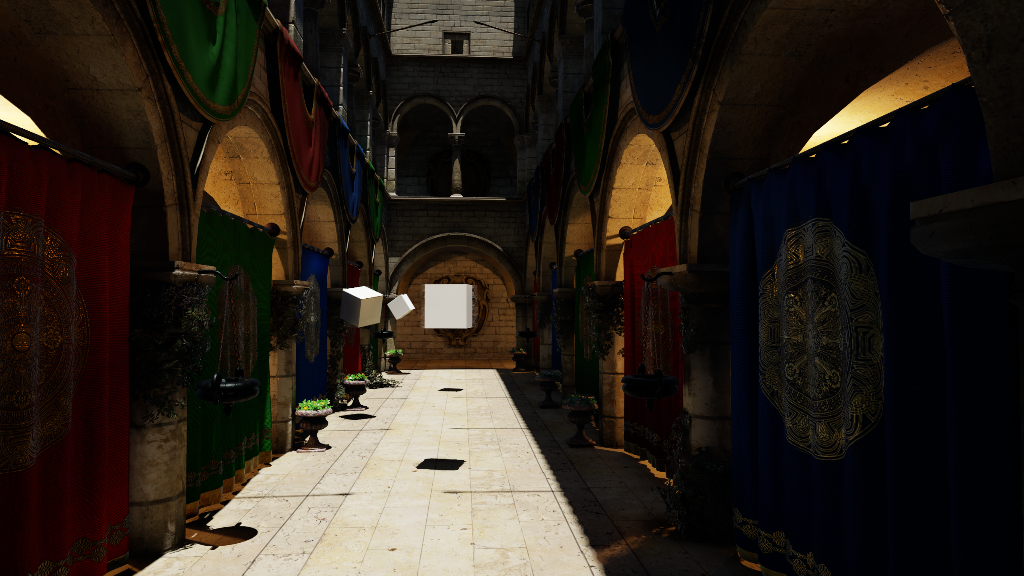
\includegraphics[width=0.92\textwidth]{figures/sponza_motion.png}
\caption[Scena kori\v{s}\'cena za merenja kretanja]{\texttt{Sponza-Motion.world}: test scena
sa \v{c}etiri rotiraju\'ca objekta dodata u visini o\v{c}iju du\v{z} glavnog broda, ovde vidljiva kao bledi kubovi i
senke koje bacaju na pod. Postoje da bi se kretali objekti, a ne samo kamera:
filter sa reprojekcijom mo\v{z}e da prati stati\v{c}nu scenu pod kretanjem kamere samo preko dubine, dok
okluder koji se nezavisno kre\'ce prisiljava filter da odbaci istoriju.}
\label{fig:sponza-motion}
\end{figure}

Prelet fiksne rute, snimanje frejmova du\v{z} nje i ocenjivanje svakog naspram konvergiranog path trace-a
istog trenutka je protokol koji je BMFR uspostavio za animirane sekvence
\cite{koskela2019bmfr}. On proizvodi upozorenje o metodi pre ikakve \v{c}injenice o rendereru: preko
jedanaest tehnika, FLIP po frejmu meren na ovaj na\v{c}in korelira sa stati\v{c}kim FLIP-om iz
Odeljka~\ref{sec:poredjenje} sa $r = +0.99$, skoro isto merenje uzeto dvaput. Konvergirani
path trace po frejmu je niz nezavisnih mirnih slika bez temporalne strukture,
jer ni\v{s}ta u njegovoj konstrukciji ne povezuje jedan frejm sa slede\'cim, pa gre\v{s}ka merena naspram njega nema
temporalnu komponentu koju bi nosila koliko god se kamera pomerala. Mana je u tom eksperimentalnom dizajnu,
a ne u implementaciji, i to je poznato mešanje: k-DOP Clipping
\cite{ikkala2024kdop} otvoreno navodi da supersamplirana referenca uvodi konstantnu gre\v{s}ku
poredi\'ci i op\v{s}ti kvalitet temporalnog antialiasinga sa supersamplingom. Kanonski radovi o denoiserima
to izbegavaju prijavljuju\'ci ta\v{c}nost naspram reference i temporalno pona\v{s}anje odvojeno,
potonje merom bez reference.

Dve veli\v{c}ine u pokretnom snimku nose informaciju koju stati\v{c}ki gejt ne mo\v{z}e. Prva poredi
koliko se tehnika menja izme\dj{}u uzastopnih frejmova naspram toga koliko se \emph{referenca}
menja u istom intervalu, pa se kretanje svojstveno sceni oduzima i ostaje samo vi\v{s}ak
nestabilnosti. Oduzimanje je bitno: na ovoj ruti se sama referenca pomera za FLIP od oko
0.09 izme\dj{}u susednih frejmova, \v{s}to bi naivna razlika frejmova prijavila kao nestabilnost. Rangirane po
njoj (Tabela~\ref{tab:motion}), tehnike se poredaju ta\v{c}no kako je proksi treperenja predvideo,
potpuno rekonstruisane konfiguracije najstabilnije, a \v{c}ista rasterizacija najmanje, \v{s}to je
zaklju\v{c}ak Odeljka~\ref{sec:denoise-eval} dostignut pod kretanjem umesto preko proksija: prostorni
filter kupuje stabilnost, a ne stati\v{c}ku vernost. Dve temporalne metrike se korisno ne sla\v{z}u:
\texttt{rtgi} ima najbolji tFLIP dok \texttt{all-rt} ima najbolji JOD, jer tFLIP izoluje
samo temporalni vi\v{s}ak, a ColorVideoVDP je prostorno-temporalan i \texttt{all-rt} je daleko ta\v{c}niji
prostorno.

\begin{table}[tbp]
\caption[Stabilnost pod kretanjem po tehnici]{Stabilnost pod kretanjem, usrednjena preko \v{c}etiri
ta\v{c}ke sonde rute (RX 9070 XT), rangirano po FLIP-u. tFLIP meri koliko se tehnika menja izme\dj{}u
susednih frejmova preko onoga koliko se sama referenca menja, \v{s}to je konstrukcija tLP iz TecoGAN-a
\cite{chu2020tecogan} sa FLIP-om umesto LPIPS-a, a kašnjenje je pokretni frejm
naspram sopstvenog konvergiranog mirnog frejma u istoj pozi. JOD je ColorVideoVDP
\cite{mantiuk2024cvvdp}, jedina mera ovde koja direktno modeluje temporalnu osetljivost na kontrast.}
\label{tab:motion}
\centering
\input{data/motion.tex}
\end{table}

Druga je kašnjenje: pokretni frejm ocenjen naspram renderer-ovog sopstvenog konvergiranog mirnog frejma u istoj
pozi, \v{s}to meri koliko rekonstrukcija zaostaje za kamerom, i \v{c}ita se du\v{z} rute u
Tabeli~\ref{tab:motion-probes} za dva kraja rang-liste. Obrtanje brzine je najskuplje
kretanje, i to ne zbog brzine, jer ruta dr\v{z}i translaciju u su\v{s}tini konstantnom: posebno kod obrtanja je to
\v{s}to vektor brzine menja znak, dokumentovan patolo\v{s}ki slu\v{c}aj za odbacivanje istorije.
Parkirana sonda je za red veli\v{c}ine ispod pokretnih i slu\v{z}i kao
kontrola koja ih \v{c}ini \v{c}itljivim.

\begin{table}[tbp]
\caption[Stabilnost i kašnjenje po sondi rute]{Iste dve temporalne mere razlo\v{z}ene po ta\v{c}ki sonde,
za krajeve rang-liste. Vrednosti se ne porede preko kolona: svaka sonda gleda razli\v{c}it
sadr\v{z}aj, pa je razlika izme\dj{}u njih uglavnom razlika u onome \v{s}to je na ekranu.}
\label{tab:motion-probes}
\centering
\input{data/motion-probes.tex}
\end{table}

Tri upozorenja idu uz ove brojeve. Ne smeju se porediti preko sondi kao da su sonde
jednako te\v{s}ke, jer svaka gleda drugi sadr\v{z}aj scene: me\dj{}u tri pokretne sonde \v{c}ista
rasterizacija ima svoj \emph{najbolji} FLIP po frejmu na sondi obrtanja, dok tamo pokazuje najgore kašnjenje. Mera kašnjenja je
renderer naspram sopstvenog mirnog frejma, pa se mo\v{z}e svesti na nulu degradiranjem mirnog frejma i nikad se ne sme
koristiti kao cilj optimizacije. A njena apsolutna skala zavisi od protokola snimanja, koji je
ispravljen tokom ovog rada, pa se smeju navoditi samo vrednosti iz trenutnih osnovnih linija i nikad mešati
sa ranijim.

\paragraph{Mere stabilnosti nagra\dj uju zamu\'cenje, a tFLIP nije izuzet.} Svaka mera koja ocenjuje rezultat
po tome koliko se malo menja izme\dj{}u uzastopnih frejmova daje prednost onom koji je izglađen, jer
je izgla\dj ivanje najjeftiniji na\v{c}in da uzastopni frejmovi li\v{c}e jedan na drugi. TecoGAN je naišao na isti
problem i zamenio razliku frejmova po pikselu perceptivnom \cite{chu2020tecogan}, \v{s}to je
konstrukcija koju tFLIP pozajmljuje. Perceptivna zamena poma\v{z}e, iako ne uklanja
sklonost: oduzimanje me\dj{}ufrejmske promene reference uklanja iz ocene kretanje same scene,
a ne zamu\'cenje tehnike, pa i stabilan rezultat i razmazan rezultat dobijaju dobru ocenu.

Ovo ovde nije hipotetičko. Dva producenta senki iz Odeljka~\ref{sec:analiza-shadow-strategy}
prostorno su nerazlu\v{c}iva na ovoj ruti, FLIP \mRtShadowFlip{} za inline putanju naspram
\mMegalightsFlip{} za stohasti\v{c}ku, a ipak ih tFLIP jasno razdvaja, \mRtShadowTflip{}
naspram \mMegalightsTflip{}, u korist stohasti\v{c}ke putanje. Upravo ta putanja se razmazuje pod kretanjem kamere,
\v{s}to je deo razloga zbog kog nije podrazumevana (Odeljak~\ref{sec:senke}). \v{C}itan sam, tFLIP bi je
preporu\v{c}io. Zato se svaki temporalni broj u ovom odeljku prijavljuje uz prostorni, i
nijedan od njih nije cilj optimizacije.

\section{Kvalitet izme\dj{}u proizvo\dj a\v{c}a}
\label{sec:cross-vendor-quality}

Me\dj{}uvendorski argument po\v{c}iva na tome da dva adaptera izvr\v{s}avaju identi\v{c}an kod, \v{s}to na drugim mestima opravdava
poređenje \emph{vremena}. Da se rekonstruisane slike tako\dj e nisu sla\v{z}ale, razlika u vremenu
uvek bi mogla da se odbaci kao posledica toga \v{s}to su dve kartice radile razli\v{c}ite koli\v{c}ine posla.

Cela matrica kvaliteta snimljena je drugi put na RTX 5070, \v{s}to daje 33 para gledi\v{s}ta i tehnike.
Preko svih 33 najve\'ca apsolutna razlika u FLIP-u izme\dj{}u adaptera je \textbf{0.0037},
medijana je \textbf{0.0007}, a 24 od 33 pada ispod 0.001. Sekundarne metrike se sla\v{z}u u
istoj meri: PSNR se nikad ne razlikuje za vi\v{s}e od 0.10 dB, a SSIM nikad za vi\v{s}e od 0.0045. Radi razmere,
razlika koja ovu glavu zaista zanima, izme\dj{}u rastera i svih uklju\v{c}enih efekata, je
FLIP od \qRasterFlip{} naspram \qAllRtFlip{}, dva reda veli\v{c}ine ve\'ca od neslaganja
proizvo\dj a\v{c}a.

Kvalitet tehnika je stoga ovde efektivno nezavisan od proizvo\dj a\v{c}a, pa je cela
me\dj{}uvendorska pri\v{c}a ovog rada o ceni, a ne o kvalitetu slike:
vremena po efektu iz Odeljka~\ref{sec:cena} i inverzija strategije senki iz
Odeljka~\ref{sec:analiza-shadow-strategy} mogu se \v{c}itati kao \v{c}iste razlike u performansama, bez
pratećeg upozorenja o kvalitetu.

Oba adaptera se ocenjuju naspram \emph{iste} path-traced reference, a o\v{c}igledna alternativa
bi poni\v{s}tila rezultat. Ke\v{s} reference je indeksiran scenom, pozom kamere, brojem frejmova i sadr\v{z}ajem
path-tracing \v{s}ejdera, a namerno ne ure\dj{}ajem, pa drugi adapter ponovo koristi referencu
koju je prvi proizveo umesto da prati sopstvenu. Da je svaki ocenjen naspram reference koju je sam proizveo,
svako poređenje bi nosilo razliku izme\dj{}u dva nezavisno konvergirana path trace-a, a nema razloga
pretpostaviti da je ta razlika mala naspram razlike tehnika koja se meri. Deljenje reference \v{c}ini
gre\v{s}ku reference zajedni\v{c}kom za obe strane, gde se poni\v{s}tava.

Dva ograni\v{c}enja uokviruju tvrdnju. Preostalo neslaganje nije nula, a najve\'ce je na
redovima ambijentalne okluzije i senki. Nepodudaranje opacity-micromap iz
Odeljka~\ref{sec:metodologija} je primamljivo obja\v{s}njenje, jer su to efekti \v{c}iji zraci
interaguju sa isecanom geometrijom, ali je malo verovatno: pe\v{c}enje micromap-a je konzervativno,
svaki mikrotrougao \v{c}iji se uzorci ne sla\v{z}u dodeljuje stanju \texttt{UNKNOWN} koje se vra\'ca na
ta\v{c}an any-hit alfa-test, pa se do rezolucije barycentric mre\v{z}e uzoraka pe\v{c}enja pogodak
razre\v{s}ava identi\v{c}no sa ekstenzijom i bez nje i menja se samo cena obilaska. Alfa
detalj u\v{z}i od te mre\v{z}e i dalje bi mogao da bude propu\v{s}ten, \v{s}to ograni\v{c}ava argument umesto da ga zatvara.
Ostatak se ovde ne pripisuje.
I referenca se ovde deli jer su oba adaptera merena na jednoj ma\v{s}ini sa toplim ke\v{s}om.
Na dve ma\v{s}ine svaka bi pratila sopstvenu, a poređenje bi zahtevalo prenos reference
umesto njenog ponovnog ra\v{c}unanja.

\section{Zauzetost i cena \v{s}ejdera}
\label{sec:occupancy}

GPU izvr\v{s}ava niti u grupama u koraku, koje se zovu wave na AMD i warp na NVIDIA, a svaka jedinica raspore\dj{}iva\v{c}a
(SIMD na AMD, SM na NVIDIA) dr\v{z}i vi\v{s}e njih rezidentnim istovremeno. Warp je 32 niti, dok
RDNA bira 32 ili 64 po \v{s}ejderu: drajver prijavljuje 64 za svaki compute \v{s}ejder u ovom engine-u, a
ne prijavljuje veli\v{c}inu za grafi\v{c}ke faze. Tabela~\ref{tab:occupancy} broji wave32 talase, a
koji od ta dva broji ne menja ono za \v{s}ta se kolona \v{c}ita, jer wave64 alocira
dvostruko ve\'ci registarski fajl i popunjava mesto sa dvostruko vi\v{s}e niti. Pri 87 i 130 registara
modeli daju 16 i 10 talasa naspram 8 i 5, \v{s}to je u oba slu\v{c}aja 512 i 320 rezidentnih niti i isti
odnos 0.625. \v{C}itanje posti\v{z}ene umesto teorijske zauzetosti zahteva hardverski profajler. Stati\v{c}ka \v{s}ejderska
zauzetost, koliko registara svaki \v{s}ejder za pra\'cenje zraka i uklanjanje \v{s}uma tra\v{z}i i koliko
talasa hardver stoga mo\v{z}e da dr\v{z}i u letu, jedino je mesto gde se dva proizvo\dj a\v{c}a porede po
ne\v{c}emu drugom osim vremenu, i obja\v{s}njava deo razlike u ceni koju ostatak glave
meri.

Hrane ga dva artefakta, namerno razli\v{c}ite te\v{z}ine. Za AMD offline analizator kompajlira
svaki \v{s}ejder i permutaciju, pa je pokrivenost potpuna i deterministi\v{c}ka, i na njemu se zasniva
gejt projekta. Za NVIDIA offline analizator ne postoji, jer se alokacija registara de\v{s}ava unutar
just-in-time kompajlera drajvera, pa se te vrednosti \v{c}itaju iz drajvera preko
\texttt{VK\_KHR\_pipeline\_executable\_properties} pošto se pipeline-i izgrade. Dva se sla\v{z}u na
svakom AMD broju registara koji dele, \v{s}to daje pravo da se oznake offline permutacija prenesu
na runtime brojeve: runtime snimak prijavljuje obe \texttt{DefaultLit} varijante pod jednim
imenom pipeline-a i ne mo\v{z}e ih sam razlikovati.

\begin{table}[tbp]
\caption[\v{S}ejderski registri i teorijska zauzetost]{Registri i teorijska zauzetost klju\v{c}nih \v{s}ejdera na obe grafi\v{c}ke kartice. Za AMD: broj VGPR-ova i
najve\'ci mogu\'ci broj wave32 talasa po SIMD-u (1536 VGPR-ova, granularnost 24, najvi\v{s}e 16). Za
NVIDIA: registri po niti i najve\'ci broj warp-ova po SM-u (65536 registara, najvi\v{s}e 48).
Obe vrednosti su izvedene iz broja registara, a ne izmerene profajlerom.
Generi\v{s}e ih \texttt{tools/gen\_shader\_tables.py} iz commitovanih osnovnih linija.}
\label{tab:occupancy}
\centering
\input{data/shader-occupancy.tex}
\end{table}

Samo jedan \v{s}ejder na putanji renderovanja je ograni\v{c}en zauzeto\v{s}\'cu na bilo kojoj kartici, i to je isti:
\texttt{DefaultLit.frag} u permutaciji sa inline senkama, sa 130 VGPR-ova i 10 od 16 talasa na
9070 XT, pa upit za senku ko\v{s}ta \v{s}est od \v{s}esnaest talasa koje bi SIMD inače mogao da dr\v{z}i rezidentnim,
vi\v{s}e od tre\'cine skupa posla dostupnog za pokrivanje kašnjenja memorije. Kompajliran bez
inline upita za senku pada na 87 VGPR-ova i punu zauzetost, \v{s}to
precizno locira cenu: pra\'cenje zraka senke unutar forward \v{s}ejdera je ono \v{s}to ga gura preko
granice talasa, isti efekat koji Odeljak~\ref{sec:cena} vidi kao Forward prolaz koji raste za \perfFwdGrowAMD{} ms.
Ni\v{s}ta u tabeli ne preliva registre, a preko svih \rgaShaderCount{} obra\dj{}enih (cooked) \v{s}ejdera ta\v{c}no jedan uop\v{s}te koristi scratch
memoriju (\texttt{NeuralConv.comp}, \rgaScratchBytes{} bajtova), van putanje renderovanja.

Slika~\ref{fig:occupancy-cliff} crta za\v{s}to dve permutacije zavr\v{s}avaju tako daleko jedna od druge za razliku od
43 registra. Zauzetost je stepenasta funkcija upotrebe registara, jer se registri alociraju u fiksnim
blokovima od 24 na ovoj arhitekturi, a broj talasa je registarski fajl podeljen tom zaokru\v{z}enom naviše
alokacijom. Izme\dj{}u 24 i 96 VGPR-ova svaki \v{s}ejder dobija svih 16 talasa, pa se pet \v{s}ejdera u ravnom
delu razlikuje u upotrebi registara za faktor 1.5 (59 do 87) bez cene u paralelizmu. Preko 96
broj pada u stepenima: permutacija sa inline senkama pri 130 VGPR-ova alocira 144 i dobija 10 talasa. Da je
ostala na 96 ili ispod, kao njen sestrinski \v{s}ejder bez pra\'cenja na 87, ne bi ko\v{s}tala ni\v{s}ta. Otuda gejt
na zauzetosti, a ne direktno na broju registara, i delovanje na pove\'canje registara samo kad
prelazi stepenik.

\begin{figure}[tbp]
\centering
\begin{tikzpicture}
\begin{axis}[width=0.86\textwidth, height=6.2cm,
  xlabel={VGPR-ova po niti}, ylabel={talasa po SIMD-u (wave32)},
  xmin=24, xmax=192, ymin=0, ymax=17.5,
  ytick={0,4,8,12,16}, xtick={24,48,72,96,120,144,168,192},
  grid=major, grid style={black!12}, tick label style={font=\small},
  label style={font=\small}]
  \addplot[const plot, thick, black] table[col sep=tab, x=vgpr, y=waves] {data/occupancy-curve.dat};
  \addplot[only marks, mark=*, mark size=1.9pt, black]
    table[col sep=tab, x=vgpr, y=waves] {data/occupancy-marks.dat};
  \node[font=\footnotesize, anchor=west] at (axis cs:130,10.9) {\texttt{DefaultLit} (inline senke)};
  \node[font=\footnotesize, anchor=east] (nobez) at (axis cs:80,13.6) {\texttt{DefaultLit} (bez)};
  \draw[black!55, thin] (nobez.east) -- (axis cs:87,15.6);
\end{axis}
\end{tikzpicture}
\caption[Zauzetost kao stepenasta funkcija broja VGPR-ova]{Teorijska zauzetost kao stepenasta funkcija broja
VGPR-ova na RDNA4 (1536 VGPR-ova, granularnost 24, najvi\v{s}e 16 talasa). Ta\v{c}ke su \v{s}ejderi iz
Tabele~\ref{tab:occupancy}. Do 96 VGPR-ova razlika u broju registara ne ko\v{s}ta ni\v{s}ta, dok
\texttt{DefaultLit} sa inline senkama pada preko granice pri 130.}
\label{fig:occupancy-cliff}
\end{figure}

Me\dj{}uvendorsko poređenje obr\'ce naivno \v{c}itanje. NVIDIA koristi znatno manje registara za
isti \v{s}ejder, 80 naspram 130 za varijantu sa inline senkama, a ipak je njena relativna zauzetost \emph{ni\v{z}a},
25 od 48 warp-ova naspram 10 od 16 talasa (52\% naspram 62\%), zbog odnosa koji svaka arhitektura
pru\v{z}a: Blackwell SM ima 65536 registara za do 48 warp-ova od 32 niti, oko 42 registra po
niti pri punoj zauzetosti, pa pritisak po\v{c}inje da se oseća ranije nego \v{s}to sirovi brojevi sugeri\v{s}u. Manje
kori\v{s}\'cenih registara ne zna\v{c}i vi\v{s}e dostupnog paralelizma.

Tri ograni\v{c}enja idu uz ove brojeve. Zauzetost je teorijska i izvedena iz registara, pa je
gornja granica za oba proizvo\dj a\v{c}a i ne govori ni\v{s}ta o onome \v{s}to se posti\v{z}e kad se uklju\v{c}e zastoji memorije i druga
ograni\v{c}enja. Za to je potreban runtime profajler. Granularnost alokacije registara RDNA4 uzeta je
iz dokumentacije, a ne potvr\dj ena izve\v{s}tajem po kompajliranju,
pa je broj talasa blizu granice zavisan od modela: pri granularnosti 8 umesto 24
permutacija sa inline senkama alocirala bi 136 registara umesto 144 i \v{c}itala 11 od 16 umesto
10. A NVIDIA vrednost je izri\v{c}ito
gornja granica, jer granularnost alokacije za tu compute sposobnost nije objavljena, a
zaokru\v{z}ivanje naviše mo\v{z}e samo da smanji broj warp-ova.

Prelivanje registara na NVIDIA namerno nije prijavljeno: drajver vra\'ca \texttt{Local Memory
Size} \v{c}iji su gornjih 32 bita konstanta, pa se vrednosti razlikuju samo u donjoj polovini, i mada je ta
donja polovina veoma verovatno stvarna vrednost, njeno maskiranje bi bilo zaklju\v{c}ivanje predstavljeno kao merenje.

\chapter{Zaklju\v{c}ak}
\label{ch:zakljucak}


\section{Rezime u odnosu na ciljeve zadatka}

Cilj zadatka, \v{c}etiri efekta osvetljenja zasnovana na pra\'cenju zrakova (senke, ambijentalna
okluzija, refleksije i difuzno globalno osvetljenje) kroz inline ray query u sopstvenom Vulkan
engine-u, uz karakterizaciju cene i kvaliteta, ostvaren je. Sva \v{c}etiri efekta dele jednu rutinu
za sen\v{c}enje pogotka nad bindless tabelom geometrije, tri koja daju \v{s}umoviti bafer dele jedan
SVGF filter za uklanjanje \v{s}uma koji se mo\v{z}e ponovo koristiti, a svi su sme\v{s}teni u postoje\'ci
rasterizacioni forward renderer, a ne u zaseban tracer (Glava~\ref{ch:implementacija}). Senke su
izuzetak koji pokazuje da dizajn radi: na podrazumevanoj putanji dva zraka po svetlu razre\v{s}avaju
vidljivost inline tokom sen\v{c}enja, dovoljno jeftino da prolaz za rekonstrukciju uop\v{s}te nije
potreban. Tabela~\ref{tab:summary} sabira klju\v{c}ne brojeve iz Glave~\ref{ch:analiza}. Obe kartice se sla\v{z}u oko najskupljeg efekta (engl.\ \perfTopEffectAMD{}), ali ga samo RX 9070 XT
odvaja od ostalih za vi\v{s}e od varijacije izme\dj u pokretanja, dok je na RTX 5070 izjedna\v{c}en
sa globalnim osvetljenjem. Razilaze se u samoj in\v{z}enjerskoj odluci: sa pet svetala u ovoj sceni stohasti\v{c}ka
strategija senki jeftinija je od dve na RX 9070 XT (\perfShadowStochAMD{} prema
\perfShadowInlineAMD{} ms), a \perfShadowRatioNV{}x skuplja na RTX 5070 (\perfShadowStochNV{} prema
\perfShadowInlineNV{} ms), pa je renderer koji fiksira bilo koju od njih pogre\v{s}an na jednoj od ove
dve kartice (Odeljak~\ref{sec:analiza-shadow-strategy}).

\begin{table}[tbp]
\caption[Rezime izmerenih rezultata]{Rezime izmerenih rezultata. Cena po efektu je razlika ukupnog
GPU vremena izme\dj u susednih konfiguracija. Kvalitet je prosek preko tri ta\v{c}ke gledi\v{s}ta u
odnosu na konvergiranu path-traced referencu na RX 9070 XT.}
\label{tab:summary}
\centering
\begin{tabular}{lrr}
\toprule
 & RX 9070 XT & RTX 5070 \\
\midrule
bazna linija bez RT (ms)  & \perfBaseAMD{}        & \perfBaseNV{} \\
senke (ms)                & \perfEffShadowsAMD{}  & \perfEffShadowsNV{} \\
AO (ms)                   & \perfEffAoAMD{}       & \perfEffAoNV{} \\
refleksije (ms)           & \perfEffReflAMD{}     & \perfEffReflNV{} \\
GI (ms)                   & \perfEffGiAMD{}       & \perfEffGiNV{} \\
\midrule
ukupno, sva \v{c}etiri (ms) & \perfTotalAMD{}     & \perfTotalNV{} \\
\midrule
FLIP: raster $\rightarrow$ ceo RT  & \multicolumn{2}{c}{\qRasterFlip{} $\rightarrow$ \qAllRtFlip{}} \\
PSNR (dB): raster $\rightarrow$ ceo RT & \multicolumn{2}{c}{\qRasterPsnr{} $\rightarrow$ \qAllRtPsnr{}} \\
SSIM: raster $\rightarrow$ ceo RT  & \multicolumn{2}{c}{\qRasterSsim{} $\rightarrow$ \qAllRtSsim{}} \\
\bottomrule
\end{tabular}
\end{table}

Koleno po broju zrakova nalazi se na jednom zraku po pikselu: prelazak sa jednog na osam zrakova
ko\v{s}ta \rcGpuPct\% vi\v{s}e GPU vremena za dobitak od \rcPsnrGain{} dB PSNR-a, koji je stvaran
(oko tri puta ve\'ci od praga merenja), ali daleko premali da opravda cenu, jer filter za uklanjanje
\v{s}uma i temporalna akumulacija ve\'c vra\'caju ve\'cinu dostizivog kvaliteta iz jednog uzorka
(Odeljak~\ref{sec:raycount}). Prostorna gustina uzoraka pona\v{s}a se isto: trasiranje GI i AO u punoj,
a ne u polovinskoj rezoluciji ko\v{s}ta \hrDeltaMs{} ms, odnosno \hrDeltaPct\% vi\v{s}e na kadru od
\hrHalfTotal{} ms, a donosi \hrPsnrGain{} dB (Odeljak~\ref{sec:halfres}). Doprinos prostornog filtera
za uklanjanje \v{s}uma tako\dj e nije tamo gde ga stati\v{c}ka metrika mo\v{z}e videti: PSNR, SSIM i FLIP
menja za manje od \v{s}uma izme\dj u pokretanja, a RMS razlike izme\dj u uzastopnih kadrova na
stati\v{c}kom pogledu smanjuje sa \flickerOff{} na \flickerOn{}, odnosno za \flickerPct\%, uz cenu od
\perfDenoiseAMD{} ms (Odeljak~\ref{sec:denoise-eval}). Pri ovom broju uzoraka rekonstrukciju radi
temporalna istorija, a prostorni filter kupuje stabilnost, a ne stati\v{c}ku vernost. Cena
ugradnje ray query-ja vidljiva je i stati\v{c}ki: na RX 9070 XT forward prolaz sen\v{c}enja sa inline
upitom za senke raste sa 87 na 130 registara po niti, \v{s}to prelazi granicu alokacije i spu\v{s}ta broj
istovremeno rezidentnih talasa sa 16 na 10, i to je jedini \v{s}ejder ograni\v{c}en zauzeto\v{s}\'cu na
putanji renderovanja na obe kartice (Odeljak~\ref{sec:occupancy}).

Prakti\v{c}na vrednost je hibridni ray query pipeline koji osvetljenje razre\v{s}ava iz geometrije
van vidnog polja kamere, \v{s}to nijedan postupak u prostoru ekrana ne mo\v{z}e, za \perfFourEffectsAMD{}
ms kadra na RX 9070 XT i \perfFourEffectsNV{} ms na RTX 5070, bez punog path tracer-a.

\section{Ograni\v{c}enja}

Merenja su obavljena na dve grafi\v{c}ke kartice uporedivog tr\v{z}i\v{s}nog ranga i na jednoj klasi
scena, pa se apsolutni brojevi ne uop\v{s}tavaju na drugi hardver ni sadr\v{z}aj. Pokrivenost
sadr\v{z}aja je najslabiji deo evaluacije po objavljenom standardu: ITU-T P.910 \cite{itu_p910}
tra\v{z}i najmanje \v{c}etiri izvorne sekvence koje obuhvataju raspon prostorne i vremenske
slo\v{z}enosti, a ovde su kori\v{s}\'cene jedna scena i dve putanje, pa artefakt specifi\v{c}an za drugi
sadr\v{z}aj ovaj protokol ne bi prona\v{s}ao. Globalno osvetljenje ograni\v{c}eno je na jedan difuzni
odskok, a senke su o\v{s}tre ili blago omek\v{s}ane, a ne fizi\v{c}ki ta\v{c}ne senke od povr\v{s}inskih
izvora. Da bi se ostalo u okviru bud\v{z}eta za rad u realnom vremenu, broj zrakova je veoma mali (jedan
ili dva po pikselu po efektu, i dva po svetlu za inline senke), \v{s}to name\'ce veliki zahtev filteru
za uklanjanje \v{s}uma i otkriva njegove na\v{c}ine otkazivanja: temporalni duh (ghosting) i
ka\v{s}njenje pri brzom kretanju, naro\v{c}ito kod refleksija, koje ponovo koriste reprojekciju
pode\v{s}enu za difuzni signal. Akceleraciona struktura najvi\v{s}eg nivoa u potpunosti se
ponovo gradi u svakom dinami\v{c}kom kadru umesto da se osve\v{z}ava, \v{s}to je za male promene
transformacija te\v{z}e nego \v{s}to je potrebno. Inline ray query-ji se odri\v{c}u hardverskog
raspore\dj ivanja zrakova i rekurzije koje bi pru\v{z}io ray tracing pipeline, \v{s}to je svesna
razmena radi jednostavnosti integracije i bila bi bitna za dublje ili brojnije odskoke.

\section{Budu\'ci rad}

Uzorkovanje je najneposredniji pravac. Stohasti\v{c}ka putanja senki ve\'c ponovo uzorkuje unutar
kadra, pa nedostaje ponovna upotreba rezervoara me\dj u susednim pikselima i izme\dj u kadrova
(ReSTIR, a za indirektne putanje ReSTIR GI), \v{s}to pri velikom broju svetala donosi kvalitet pri
istom broju zrakova \cite{bitterli2020restir, ouyang2021restirgi}. Uzorkovanje hemisfere sa
kosinusnom te\v{z}inom u osnovi GI i AO tim radom ostaje netaknuto i naivno. Kod rekonstrukcije,
nau\v{c}eni filter za uklanjanje \v{s}uma ili skaliranje koji zamenjuje ili dopunjuje SVGF prirodan
je slede\'ci korak. Sama stohasti\v{c}ka strategija senki prototip je, a ne zavr\v{s}ena tehnika:
da bi postala podrazumevana, prvo bi trebalo ukloniti artefakte koje pokazuje pri kretanju kamere
tamo gde se dva ta\v{c}kasta svetla preklapaju. Posebni filter za senke koji uzima u obzir
polusenku, umesto zajedni\v{c}kog, srodno je pobolj\v{s}anje. \v{S}ire cross-vendor pore\dj enje
od dve kartice aktuelne generacije, kao i drugi renderski backend (DirectX 12), dodatno bi
pro\v{s}irili sliku o performansama.


% Manual bibliography, hand-formatted to PPK's citation style, ordered by citation.
\clearpage
\phantomsection
\addcontentsline{toc}{chapter}{\bibname}
% Bibliography in PPK format (Prezime Ime, „Naslov,“ izdanje/venue, izdavac, mesto, godina),
% ordered by citation. Hand-formatted; this list is the only bibliography, there is no BibTeX step.
\begin{thebibliography}{99}

\bibitem{mittring2007cryengine}
Mittring Martin, \rqt{Finding Next Gen: CryEngine 2}, SIGGRAPH Courses, 2007.

\bibitem{bavoil2008hbao}
Bavoil Louis, Sainz Miguel, Dimitrov Rouslan, \rqt{Image-Space Horizon-Based Ambient Occlusion},
SIGGRAPH Talks, 2008.

\bibitem{crassin2011vxgi}
Crassin Cyril, Neyret Fabrice, Sainz Miguel, Green Simon, Eisemann Elmar, \rqt{Interactive Indirect
Illumination Using Voxel Cone Tracing}, Computer Graphics Forum (Pacific Graphics), 2011.

\bibitem{kajiya1986rendering}
Kajiya James T., \rqt{The Rendering Equation}, SIGGRAPH, 1986.

\bibitem{schied2017svgf}
Schied Christoph, Kaplanyan Anton, Wyman Chris, Patney Anjul, Chaitanya Chakravarty R. Alla, Burgess
John, Liu Shiqiu, Dachsbacher Carsten, Lefohn Aaron, Salvi Marco, \rqt{Spatiotemporal Variance-Guided
Filtering: Real-Time Reconstruction for Path-Traced Global Illumination}, High Performance Graphics
(HPG), 2017.

\bibitem{moller1997raytri}
M\"oller Tomas, Trumbore Ben, \rqt{Fast, Minimum Storage Ray/Triangle Intersection}, Journal of
Graphics Tools, 1997.

\bibitem{pharr2016pbrt}
Pharr Matt, Jakob Wenzel, Humphreys Greg, \rqt{Physically Based Rendering: From Theory to
Implementation}, tre\'ce izdanje, Morgan Kaufmann, 2016.

\bibitem{akenine2018rtr}
Akenine-M\"oller Tomas, Haines Eric, Hoffman Naty, Pesce Angelo, Iwanicki Micha\l{}, Hillaire
S\'ebastien, \rqt{Real-Time Rendering}, \v{c}etvrto izdanje, A K Peters/CRC Press, 2018.

\bibitem{khronos_rayquery}
The Khronos Group, \rqt{Vulkan Specification: \texttt{VK_KHR_ray_query},
\texttt{VK_KHR_acceleration_structure}}, \url{https://registry.khronos.org/vulkan/}, pristupano 2026.

\bibitem{majercik2019ddgi}
Majercik Zander, Guertin Jean-Philippe, Nowrouzezahrai Derek, McGuire Morgan, \rqt{Dynamic Diffuse
Global Illumination with Ray-Traced Irradiance Fields}, Journal of Computer Graphics Techniques
(JCGT), 2019.

\bibitem{nvidia_rtxgi}
NVIDIA, \rqt{RTX Global Illumination (RTXGI)}, \url{https://developer.nvidia.com/rtxgi}, pristupano
2026.

\bibitem{epic_lumen}
Epic Games, \rqt{Lumen Global Illumination and Reflections}, Unreal Engine Documentation,
\url{https://docs.unrealengine.com/}, pristupano 2026.

\bibitem{bitterli2020restir}
Bitterli Benedikt, Wyman Chris, Pharr Matt, Shirley Peter, Lefohn Aaron, Jarosz Wojciech,
\rqt{Spatiotemporal Reservoir Resampling for Real-Time Ray Tracing with Dynamic Direct Lighting}, ACM
Transactions on Graphics (SIGGRAPH), 2020.

\bibitem{ouyang2021restirgi}
Ouyang Y., Liu S., Kettunen M., Pharr M., Pantaleoni J., \rqt{ReSTIR GI: Path Resampling for
Real-Time Path Tracing}, Computer Graphics Forum (HPG), 2021.

\bibitem{schied2018asvgf}
Schied Christoph, Peters Christoph, Dachsbacher Carsten, \rqt{Gradient Estimation for Real-Time
Adaptive Temporal Filtering}, ACM on Computer Graphics and Interactive Techniques (HPG), 2018.

\bibitem{nvidia_nrd}
NVIDIA, \rqt{Real-Time Denoisers (NRD)},
\url{https://developer.nvidia.com/rtx/ray-tracing/rt-denoisers}, pristupano 2026.

\bibitem{intel_oidn}
Intel, \rqt{Open Image Denoise (OIDN)}, \url{https://www.openimagedenoise.org/}, pristupano 2026.

\bibitem{karis2014taa}
Karis Brian, \rqt{High Quality Temporal Supersampling}, SIGGRAPH Courses: Advances in Real-Time
Rendering in Games, 2014.

\bibitem{ikkala2024kdop}
Ikkala Joel, Aittala Miika, Laine Samuli, Lehtinen Jaakko, \rqt{k-DOP Clipping: Robust Temporal
Antialiasing}, SIGGRAPH Asia, 2024.

\end{thebibliography}


\end{document}
